\documentclass{sig-alternate}
%\usepackage{amsthm}
\usepackage{amsmath}
\usepackage{xspace}
\usepackage{times}
\usepackage{algorithmicx}
\usepackage{cite}
\usepackage{color}
%% Jeppe:        63835584


\usepackage[noend]{algpseudocode}
\usepackage{algorithm}
%\usepackage[caption=false]{subfig}
%\usepackage{multirow}

\newcommand{\stitle}[1]{\vspace*{0.4em}\noindent{\bf #1:\/}}
\newcommand{\sntitle}[1]{\vspace*{0.4em}\noindent{\bf  #1\/}}
\newcommand{\sstitle}[1]{\vspace*{0.4em}\noindent{\bf #1\/.}$\\$ }
\newtheorem{definition}{Definition}
\newtheorem{problem}{Problem}
\newtheorem{lemma}{Lemma}


\sloppy

\pagestyle{plain}


\newcommand{\ffh}[1]{\textbf{TODO: \textit{#1}}}


\newcommand{\spath}{SP\xspace}
\newcommand{\zebox}[1]{$|\underline{\overline{#1}}|$}



\begin{document}



\title{Effective Caching of Shortest Paths for Location-Based Services}

%% Authors: Jeppe, Ken, Christian


\maketitle

\begin{abstract}
%short description of what we do, why this is an interesting/challenging problem, and how well we solve the problem (key results, mention theoretical guaranties.)
%
Web search is ubiquitous in our daily lives.
Caching have been extensively used to reduce the computation time of the search engine
and reduce the network traffic beyond a proxy server.
Another form of web search, known as online shortest path search, is popular due
to advances in geo-positioning.
However, existing caching techniques are ineffective for shortest path queries.
This is due to several crucial differences
between web search results and shortest path results, in relation to query matching,
cache item overlapping, and query cost variation.

Motivated by this, we identify several properties that are essential to the success of effective
caching for shortest path search.
Our cache exploits the optimal subpath property, which allows a cached shortest path to answer
any query with source and target nodes on the path.
We utilize statistics from query logs to estimate the benefit of caching a specific shortest path,
and we employ a greedy algorithm for placing beneficial paths in the cache.
Also, we design a compact cache structure that supports efficient query matching at runtime.
Empirical results on real datasets confirm the effectiveness of our proposed techniques.
\end{abstract}

%%% content here ...




\section{Introduction} \label{sec:intro}
%
Web search is ubiquitous and extensively used in our daily lives.
The scenario for typical web search is illustrated in Figure~\ref{fig:arch}.
A user may submit a query ``Paris Eiffel Tower'' to the search engine,
which then computes relevant results and reports them back to the user.
Usually, a {\em cache} is used to keep the results of frequent queries
in order to achieve a high hit ratio~\cite{BaezaYates07,OzcanAU08,AltingovdeOU09,Ozcan2011}.
%  where is a cache?
The cache can be employed at the search engine to save its computation time,
e.g., when the query (result) can be found in the cache.
%
To improve response time, a cache can also be placed at a proxy that
resides in the same sub-network as the user.
A query result that is available at the proxy can be reported immediately, without contacting the search engine.
% what content in a cache?  and the goal



\begin{figure}[hbt]
  \center
        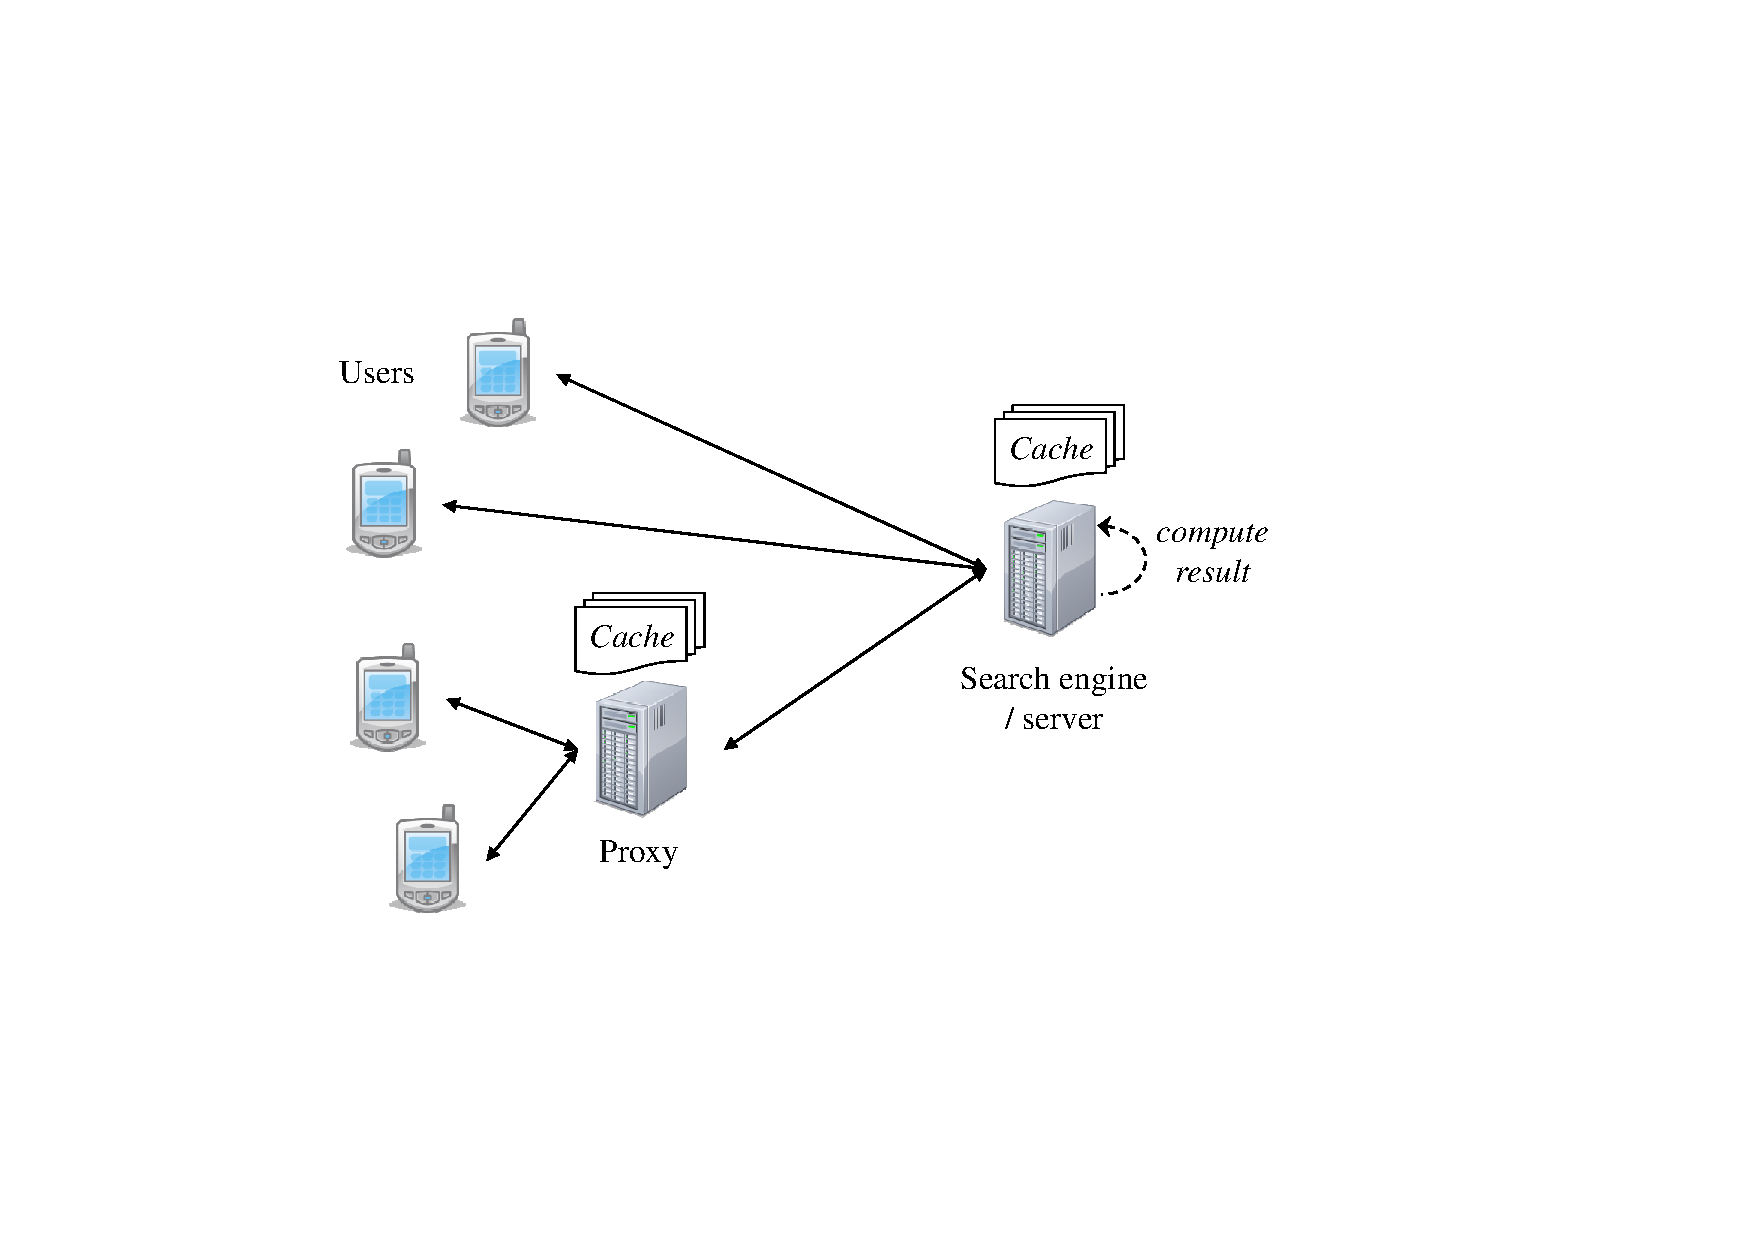
\includegraphics[width=0.7\columnwidth]{figures/scenario}
        \caption{Scenario for Web Search}
  \label{fig:arch}
\end{figure}

%  note:  emphasize the concepts of  cache location
%  service provider, reduce SP computation cost
%  proxy, reduce communication cost


%It consists of three types of entities: the path server, proxy, and clients (mobile devices).
%Some user may contact the path finder server directly for service.
%Some user may contact the path finder server via some proxy.

The scenario of Figure~\ref{fig:arch} is applicable to {\em online shortest path search} on a map as well,
which are popular due to advances in geo-positioning capability of mobile devices (e.g., PDA, smartphone).
%enable users to search for shortest paths from their current locations to their destinations.
It has various applications for mobile users, e.g., a tourist asking for directions to a museum,
a driver finding the route to a gas station, and a customer wanting to reach a restaurant.
%
%offline
When compared to offline commercial navigation software, online search (e.g., Google Maps, MapQuest)
provide two benefits to mobile users:
(i) they are free to use, and
(ii) they do not require any installation and storage space at mobile devices.
% the map data is asset (hard to argue)
%growing importance

Figure~\ref{fig:rxmap} shows a road network in which a node $v_i$ is a road junction
and an edge $(v_i,v_j)$ models a road segment with its distance %$W(v_i,v_j)$
shown as a number.
The shortest path from $v_1$ to $v_7$ is the path $\langle v_1, v_3, v_4, v_5, v_7 \rangle$
and its path distance is $3+6+9+5=23$.
%
Again, caching can be utilized at a proxy to reduce the response time,
or it can be used at the server to reduce the server's computation time.


%%  CSJ (obtained from meeting with GIS people): Route computation was a solved issue because existing techniques are really fast.
% try to do back-of-the-envelope estimations of what it will cost (latency, computation time) to compute routes
% without caching and with caching according to state of the art techniques.

% (They are very efficient, able to compute a shortest path in a few milliseconds only.)


%% Ken
%
%Our current implementation of the shortest path cache involves some
%runtime overhead and it takes more time than a few milliseconds to answer a query.
%
%Perhaps it doesn't make sense to use such a cache at the service provider.
%
%In your opinion, would it be reasonable to use a cache at the proxy server ?
%( The average Internet round-trip-time is 1 second. )



{\bf +++ CSJ: Yes, it may be wise to emphasize the proxy part so that we aim to reduce the Internet latency. Then we may want to understand/explain in a bit more detail how proxies are used today for Internet search.}



\begin{figure}[hbt]
  \center
        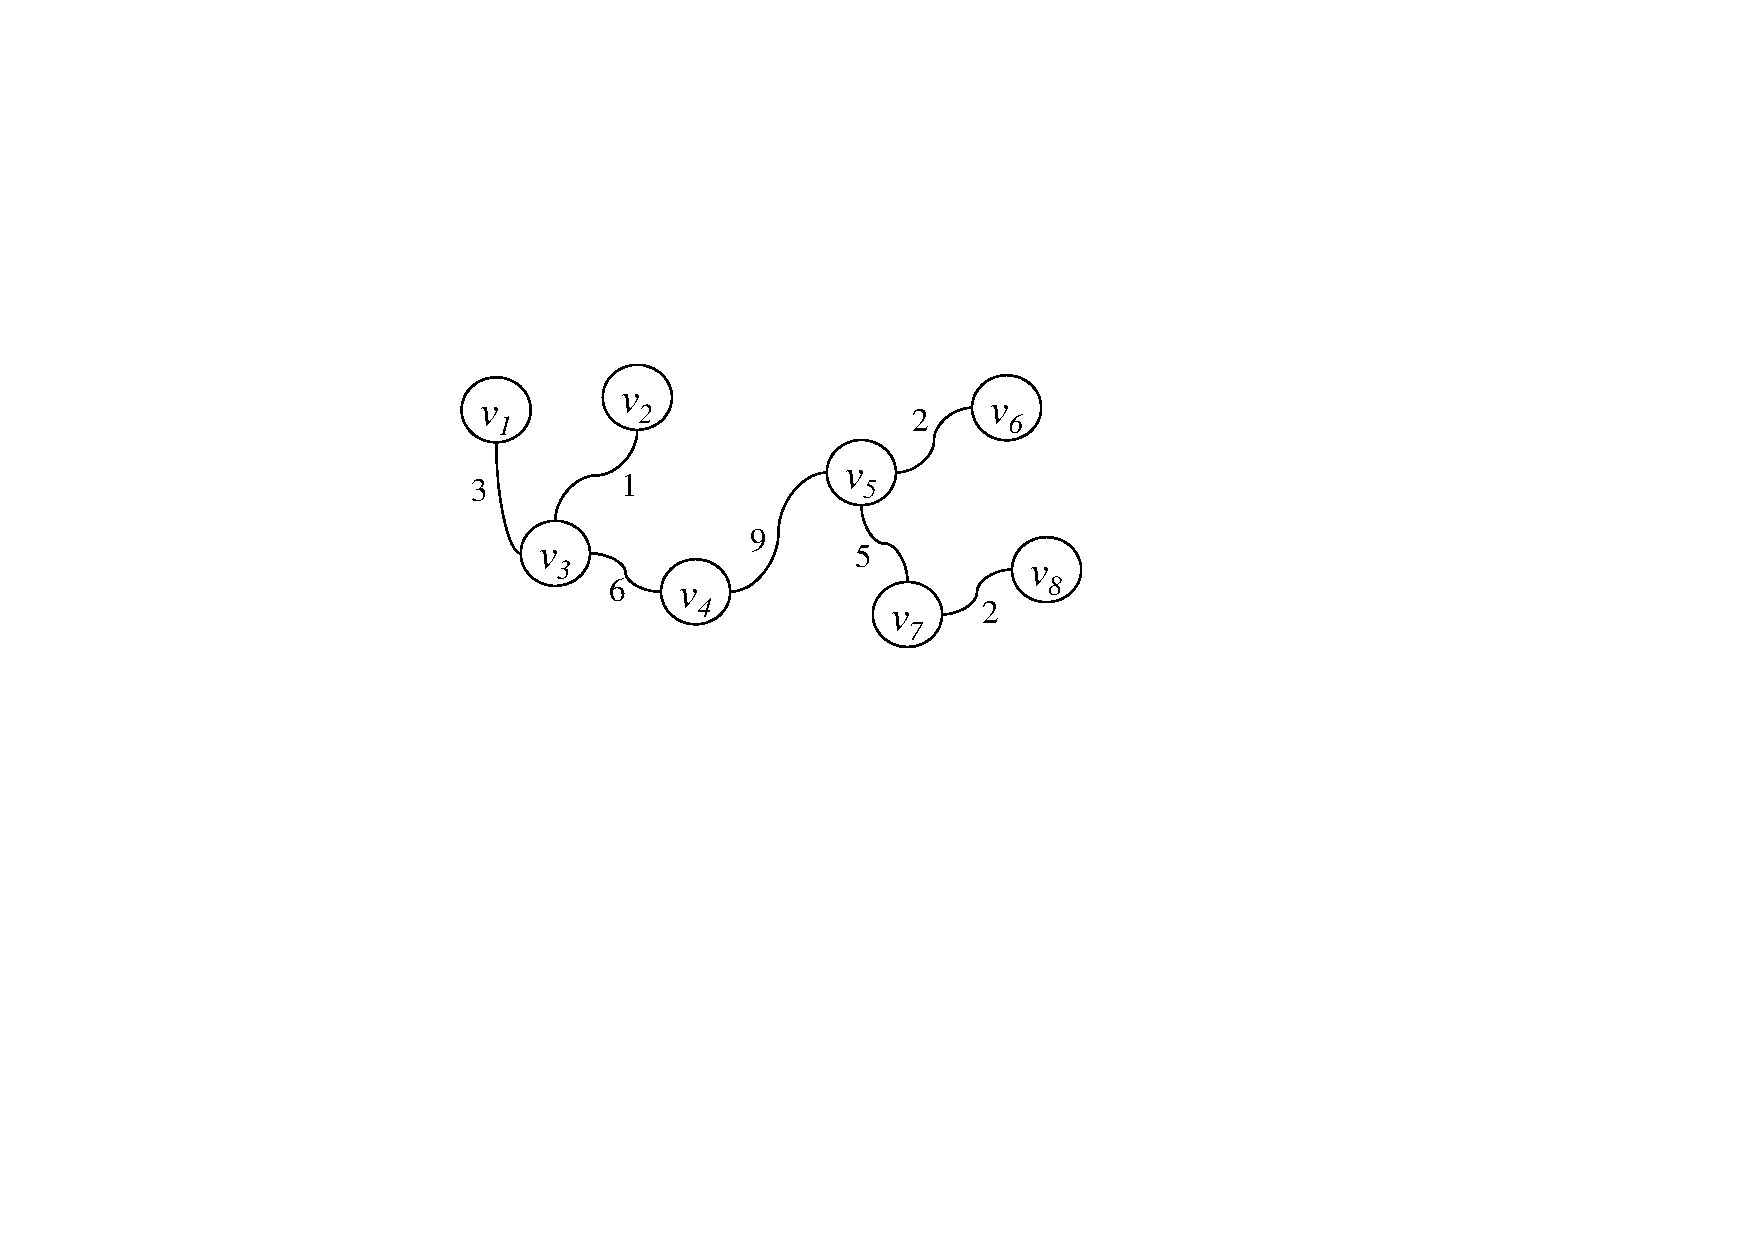
\includegraphics[width=0.7\columnwidth]{figures/rxmap}
        \caption{An Example Road Network}
  \label{fig:rxmap}
\end{figure}


We study the caching of path search results in a scenario as shown in Figure~\ref{fig:arch}.
Nevertheless, there are crucial differences between general web search results and shortest path results,
rendering existing caching techniques for web results ineffective in our context.
\begin{itemize}
    \itemsep -2pt
    \item {\bf Exact matching vs. subpath matching:} The result of a web query (e.g., ``Paris Eiffel Tower'') seldom matches with that of another query (e.g., ``Paris Louvre Palace''). In contrast, a shortest path result contains subpaths that can be used for answering other queries. For example, the shortest path from $v_1$ to $v_7$ ($\langle v_1, v_3, v_4, v_5, v_7 \rangle$) contains the shortest path from $v_3$ to $v_5$, the shortest path from $v_4$ to $v_7$, etc. We need to re-visit the model for defining the benefit of a path.
    \item {\bf Cache structure:} Web search caching may employ a hash table to check efficiently whether a query can be found in the cache. However, such a hash table cannot support the subpath matching found in our setting. A new structure is required to organize the cache content in an effective way for supporting subpath matching.
        %
        Furthermore, this problem is complicated by the overlapping of paths. For example, the shortest path $\langle v_1, v_3, v_4, v_5, v_7 \rangle$ and the shortest path $\langle v_2, v_3, v_4, v_5, v_6 \rangle$ have significant overlap, although each of them does not contain the other. It is challenging to develop a compact structure for storing these paths.
        % hash table suffices ...
    \item {\bf Query processing cost:}
        At the server side, when a cache miss occurs, an algorithm is invoked to compute the query result.
%        For the server scenario, the goal of the cache is to reduce the total time of processing queries.
        Some results are more expensive to obtain than other results.
        %The benefit of a cached result is decided not only by its frequency, but also by the time to compute it.
        %
        To optimize the server performance, a cost model has been developed for estimating the cost of a web query~\cite{AltingovdeOU09},
        in order to decide the importance of a result.
        However, to our knowledge, there is no work on estimating the cost of a shortest path query
        with respect to a given shortest path algorithm.
%        We observe that the cost of processing a query is not static, rat
%    \item {\bf Optimization goal:} The optimization goal in our caching problem depends on the location of the cache. For a cache placed at a proxy, the optimization goal is still the hit ratio. However, for a cache placed at the server, the optimization goal is the running time, which heavily depends on the shortest path distance and the underlying algorithm. We need a model to estimate the cost of computing a specific shortest path, in order to determine the potential benefit of caching it.
\end{itemize}
%
% web caching is a better target to attack
% these challenges are better than just arguing with LRU ...


%Introduce problem and a running example to use throughout the paper.
%clarify why we need to solve this problem.

%Challenges:
%\begin{itemize}
%\item
%\item Searching the cache must be faster than calculating a \spath.
%\item Needs to use small amount of space to achieve a good cache hit ratio.
%\item
%\end{itemize}



% cost of a shortest path search algorithm ...
% consider Dijkstra just because of a cost model ...
%enable users to acquire their geo-positions and enjoy location-based services conveniently.
%  third reason:  navigation software is forced to download map updates regularly  (but our method can't handle static map)



%To our best knowledge, we are the first to tackle the caching


In order to tackle the above challenges, we make the following contributions:
\begin{itemize}
    \itemsep -2pt
    \item We formulate a systematic model for quantifying the benefit of caching a specific shortest path.
    \item We design techniques for extracting statistics from query logs
          and benchmarking the cost of a shortest path call.
    \item We propose an algorithm for selecting paths to be placed in the cache.
    \item We develop a compact and efficient cache structure for storing shortest paths.
    \item We study the above contributions empirically using real data.
\end{itemize}


The rest of the paper is organized as follows.
Section~\ref{sec:relwork} studies the work related to the shortest path caching problem.
Section~\ref{sec:problem} defines our problem formally, and
Section~\ref{sec:BenefitDriven} formulates a model for capturing the benefit of a cached shortest path,
examines the query frequency and the cost of a shortest path call, and presents an algorithm for selecting
appropriate paths to be placed in the cache.
Section~\ref{sec:CacheStruct} presents a compact and efficient cache structure for storing shortest paths.
Our proposed methods are then evaluated on real data in Section~\ref{sec:experiments},
followed by a conclusion in Section~\ref{sec:conclusion}.






% another challenge: huge number of paths (put it in another section?)
%    The number of possible \spath candidates to add to the cache are $|V|^2$. $|V|$ is the number of nodes in a road network.







\section{Related Work} \label{sec:relwork}
%
%Introduce related work, group them by similar work and tell what they do and why their approaches can not solve our problem.


\stitle{Web Search Caching}
%
A web search query asks for the top-$K$ relevant documents (i.e., web pages)
that best match a text query, e.g., ``Paris Eiffel Tower''.
The typical value of $K$ is the number of results (e.g., 10) to be displayed on a result page~\cite{Ozcan2011};
a request for the next result page is interpreted as another query.
% top-$K$ ($K$=50, over 95\% of queries need up to 3 pages of results)
% inverted index,  posting list for each term, document id
% query   % a document: highest scores
% top-k result:
% a web search result
%\cite{Markatos01}

Web search caching is used to improve the performance of a search engine.
When a query can be answered by the cache, the cost of computing the query result can be saved.
%Existing work on web search caching take different approaches in three aspects:
%(i) the mode of cache update, (ii) the type of items to be cached, and (iii) the performance measurement.
%
% optimization goal (cache policy)
%
Markatos et al.~\cite{Markatos01} present pioneering work on evaluating two caching approaches
(dynamic caching and static caching) on real query logs.
{\em Dynamic caching}~\cite{Markatos01,LongS05,GanS09} aims to cache the results of the most recently accessed queries.
For example, in the Least-Recently-Used (LRU) method,
when a query causes a cache miss, the least recently used result in the cache will be replaced by the current query result.
This approach keeps the cache up-to-date and adapts quickly to the distribution of the incoming queries;
however, it incurs the overhead of updating the cache frequently.
%
On the other hand, {\em static caching}~\cite{Markatos01,BaezaYates03,BaezaYates07,AltingovdeOU09,OzcanAU08,Ozcan2011}
aims to cache the results of the most popular queries.
It exploits a query log, which contains past users' queries in the past, to determine the most frequent queries.
The above studies have shown that
the frequency of queries follows Zipfian distribution, i.e., a small number of queries
have very high frequency, and they remain popular for a period of time.
Although the cache content is not the most up-to-date, it is able to answer the majority of frequent queries.
A static cache can be updated periodically (e.g., every day) based on the latest query log.
Static caching has the advantage that it incurs very low overhead at query time.
%the query frequency is stable within a month.
%static caching \cite{Markatos01,BaezaYates07,AltingovdeOU09,OzcanAU08,Ozcan2011}
%dynamic caching


%results~\cite{Markatos01,OzcanAU08,GanS09}
%
% what is a posting list
%posting lists~\cite{BaezaYates03}
%results, intersection of posting lists, posting lists~\cite{LongS05}
% CPU time


Early works on web search caching adopt the {\em cache hit ratio} as the performance metric.
This metric reflects the number of queries that do not require computation cost.
%
Recent work~\cite{BaezaYates07,AltingovdeOU09,Ozcan2011} on web search caching use the {\em server processing time} as the performance metric.
They show that different queries have different query processing times.
For example, a query that involves terms with large posting lists is expected to incur high cost.
Refs.~\cite{AltingovdeOU09,Ozcan2011} propose models for estimating the cost of processing queries
based on the sizes of inverted lists, and they exploit both frequency and cost information in static caching methods.
% cost and frequency
%then present static caching methods that fill the cache
%with result
%   frequency and processing cost of queries.
%  cost model~, disk access and CPU time, estimated based on the lengths of posting lists

%necessary to explain static caching and dynamic caching
% and their benefits

%mention some heuristics used for filling a static cache



% Important: SIGIR 2007 paper talks about "static caching"



% see if any other paper is needed


None of the above works have studied the caching of shortest paths.
In this paper, we adopt a static caching approach
%to cache query results
because it performs well on query logs that are typically skewed in nature and incurs very low overhead at query time.
The cost models of \cite{AltingovdeOU09,Ozcan2011} are specific to web search queries
and are inapplicable to our problem.
In our caching problem, different shortest path queries also have different processing times.
Thus, we will study a cost-oriented model for quantifying the benefit of placing a specific path in the cache.
%  the best paths to be placed in the cache.



\stitle{Semantic Caching}
%
% Client-side caching has also been studied in client-server systems.
In a client-server system, a cache may be employed at the client-side in order to reduce the communication cost
and improve response latency of the client.
The cache located at a client can only serve queries from the client itself, not from other clients.
%The content of the cache is dedicated to the client and it ca
Such a cache is only beneficial for a query-intensive user. %, but not for a service with multiple users.
All techniques in this category adopt the dynamic caching approach.
%% serve a single client ...

Semantic caching~\cite{DarFJST96} is a client-side caching model that associates cached results with valid ranges.
%Subsequent queries can be answered partially by a cached result and
Upon receiving a query $Q$, the relevant results from the cache are reported.
A subquery $Q'$ is constructed from $Q$ such that $Q'$ covers the query region that cannot be answered by the cache.
The subquery $Q'$ is then forwarded to the server in order to obtain the remaining results of $Q$.
Ref.~\cite{DarFJST96} focuses on semantic caching of relational datasets.
As an example, assume that the dataset stores the age of each employee
and that the cache contains the result of the query ``find employees with age below 30''.
Now assume that the client issues a query $Q$ ``find employees with age between 20 and 40''.
First, the employees with age between 20 and 30 can be obtained from the cache.
Then, a subquery $Q'$ ``find employees with age between 30 and 40'' is submitted to server for retrieving
the remaining results.


Semantic caching has also been studied for spatial data~\cite{ZhengL01,pcsqm,ccslbs}.
% and image data~\cite{ccqreir,nnccma}.
Zheng et al.~\cite{ZhengL01} define the semantic region of a spatial object as its Voronoi cell,
which can then be utilized to answer nearest neighbor queries for a moving client user.
Hu et al.~\cite{pcsqm} study semantic caching of tree nodes in an R-tree and
examine how to process generic spatial queries on the cached tree nodes.
Lee et al.~\cite{ccslbs} build generic semantic regions for spatial objects so that
they are able to support generic spatial queries.
However, no semantic caching techniques for graphs or shortest paths have been proposed.


%Furthermore, semantic caching is only suitable for a client with intensive queries,
%but it cannot be not applicable to




%% differentiate, why not semantic caching


%% none of the work on graph



%\stitle{Path Caching in Networking}
%%
%get the references from home ...
%
%
%\cite{csptri} \cite{spcrtp}


\stitle{Shortest Path Computation}
%
Existing shortest path indexes can be categorized into three types,
which represent different trade-offs between their precomputation effort and query performance.
%
A basic structure is the adjacency list, in which each node $v_i$ is assigned a
list for storing the adjacent nodes of $v_i$. It does not store any pre-computed information.
Uninformed search (e.g., Dijkstra's algorithm, bidirectional search) can be used to
compute the shortest path; however, it incurs high query cost.
%
{\em Fully-precomputed} indexes, e.g., the distance index~\cite{HuLL06} or
the shortest path quadtree~\cite{SametSA08}, require precomputation of the shortest paths between any two nodes in the graph.
Although they support efficient querying, they incur huge precomputation time ($O(|V|^3)$)
and storage space ($O(|V|^2)$), where $|V|$ is the number of nodes in the graph.
%
%These methods are only applicable to small graphs, as they lead to very high precomputation
%cost and storage overhead.
{\em Partially-precomputed} indexes, e.g., landmarks~\cite{Kriegel08}, HiTi~\cite{jung02}, and TEDI~\cite{Wei10},
attempt to materialize some distances/paths in order to accelerate the processing of shortest path queries.
They employ some parameter to control the trade-offs among query performance, precomputation overhead, and storage space.

%  discuss about the indexes
%  orthogonal to the algorithm ...





As a possible approach to our caching problem,
one could assume that a specific shortest path index is being used at the server.
A portion of the index may be cached so that it can be used to answer certain queries rapidly.
% Then, the objective of this approach would be to cache a part of the index.
Unfortunately, this approach is tightly coupled to the assumed index, and
it is inapplicable to servers that employ other indexes.
Also, it cannot be applied directly to any new index developed in the future.


In this paper, we view the shortest path index/algorithm as a black-box
and decouple it from the cache.
%so we are not allowed to exploit the internal structure of the index.
The main advantage is that our approach is applicable to any shortest path method,
without knowing its implementation. Any new shortest path method can be
integrated with our proposed cache seamlessly.



%explain why black-box

%possible to cache part of the index, but need query specific algorithm

%when a new shortest path index is published, a new caching technique needs to be designed

%we want a generic caching technique for shortest paths




\section{Problem Setting}\label{sec:problem}
%
We first introduce some background definitions and properties.
Then we present our problem and objectives.
Table~\ref{tbl:symbols} summarizes the notations to be used in this paper.

\begin{table}[hbt]
\center
\begin{tabular}{|c|c|}
    \hline
    \bf Notation & \bf Meaning \\\hline
    $G(V,E)$ 	& a graph with node set $V$ and edge set $E$ \\\hline
    $v_i$ 		& a node in $V$ \\\hline
    $(v_i,v_j)$  & an edge in $E$ \\\hline
    $W(v_i,v_j)$  & the edge weight of $W(v_i,v_j)$ \\\hline
    $Q_{s,t}$		& shortest path query from node $v_s$ to node $v_t$ \\\hline
    $P_{s,t}$		& the shortest path result of $Q_{s,t}$ \\\hline
    $|P_{s,t}|$		& the size of $P_{s,t}$ (in number of nodes) \\\hline
    $E_{s,t}$		& the expense of executing query $Q_{s,t}$ \\\hline
    $\chi_{s,t}$		& The frequency of a \spath \\\hline
    $\Psi$ 			& the cache \\\hline
    $\mathfrak{U}(P_{s,t})$		& the set of all subpaths in $P_{s,t}$ \\\hline
    $\mathfrak{U}(\Psi)$	& the set of all subpaths of paths in $\Psi$ \\\hline
    $\gamma(\Psi)$	& the total benefit of the content in the cache \\\hline
    $\mathcal{QL}$	& query log  \\\hline
\end{tabular}
\caption{Summary of Notations}
\label{tbl:symbols}
\end{table}


\subsection{Definitions and Properties}
%
We first provide the definitions of graph and shortest path.
%
\begin{definition}
{\bf Graph model. $\\$}
%
Let $G(V,E)$ be a graph with a set $V$ of nodes and a set $E$ of edges.
Each node $v_i \in V$ models a road junction.
Each edge $(v_i,v_j) \in E$ models a road segment, and its length is denoted as $W(v_i,v_j)$.
%
\end{definition}
\begin{definition}
{\bf Shortest path: query and result. $\\$}
%
A shortest path query, denoted by $Q_{s,t}$, consists of a source node $v_s$ and a target node $v_t$.

The result of $Q_{s,t}$, denoted by $P_{s,t}$, is the path from $v_s$ to $v_t$ (on graph $G$)
with the minimum sum of edge weights (lengths) along the path.
%
We can represent $P_{s,t}$ as a list of nodes: $\langle v_{x_0}, v_{x_1}, v_{x_2} \cdots, v_{x_m} \rangle$,
where $v_{x_0}=s$, $v_{x_m}=t$, and the path distance is: $\sum_{i=0}^{m-1} W(v_{x_i},v_{x_{i+1}})$.
\end{definition}

We consider only undirected graphs in our examples.
Our techniques can be easily applied to directed graphs.
In the example graph of Figure~\ref{fig:rxmap},
the shortest path from $v_1$ to $v_7$ is the path $P_{1,7}=\langle v_1, v_3, v_4, v_5, v_7 \rangle$
with its length $3+6+9+5=23$.




Shortest paths exhibit the optimal subpath property (see Lemma~\ref{lem:oss}).
It states that every subpath of a shortest path is also a shortest path. For example, in Figure~\ref{fig:rxmap},
the shortest path $P_{1,7}=\langle v_1, v_3, v_4, v_5, v_7 \rangle$
contains these shortest paths: $P_{1,3}, P_{1,4}, P_{1,5}, P_{1,7}$, $P_{3,4},P_{3,5}, P_{3,7}$, $P_{4,5}, P_{4,7}, P_{5,7}$.
%
As we will discuss shortly, this property can be exploited for caching shortest paths.

%which means that any \spath in the cache can answer any \spath query where both origin and target node are on the \spaths. Calculating which \spaths, and their subpaths, provide the most benefit will obviously be necessary for optimal utilization of the cache.




%A static cache, which is populated in an offline phase (fig. \ref{fig:routequery}E), is used. A static cache will impose minimal overhead to query processing. Section \ref{sec:competitors} explains why we choose a static cache.



\begin{lemma}\label{lem:oss}
{\bf Optimal subpath property (from~\cite{introalg}). $\\$}
%
The shortest path $P_{a,b}$ contains the shortest path $P_{s,t}$
if $s \in P_{a,b}$ and $t \in P_{a,b}$.
%
Specifically, let $P_{a,b}=\langle v_{x_0}, v_{x_1}, v_{x_2} \cdots, v_{x_m} \rangle$.
We have $P_{s,t}=\langle v_{x_i}, v_{x_{i+1}}, \cdots, v_{x_j} \rangle$ if $s=v_{x_i}$ and $t=v_{x_j}$.
\end{lemma}




\subsection{Problem and Objectives}\label{subsec:goals}
%
% reuse the architecture in intro
We adopt the architecture of Figure~\ref{fig:arch} to our caching problem.
Using mobile devices with geo-positioning capabilities, users issue shortest path queries to an online server.
The cache, as defined below, can be placed at either a proxy or the server.
It helps improve the computation cost and the communication cost at the server/proxy,
as well as reduce the response time of shortest path queries.
\begin{definition}
{\bf Cache and budget. $\\$}
%
Given a cache budget $\mathcal{B}$, a cache $\Psi$ is allowed to store a collection of shortest path results such that
$|\Psi| \le \mathcal{B}$, where the cache size $|\Psi|$ is taken as the total number of nodes of shortest paths in $\Psi$.
%
\end{definition}
%static caching vs. dynamic caching
As discussed in Section~\ref{sec:relwork},
recent literature on web search caching~\cite{BaezaYates07,AltingovdeOU09,OzcanAU08,Ozcan2011}
advocates the use of a static cache rather than a dynamic cache.
Static caching has very low runtime overhead, while it only sacrifices the hit ratio a little.
Thus, we also adopt the static caching paradigm and exploit a query log to build a cache.
\begin{definition}
{\bf Query log. $\\$}
%
A query log $\mathcal{QL}$ is a collection of timestamped queries that have been
issued by users in the past.
%
\end{definition}

%{\bf ++ what static and dynamic cachingare and how they differ}

%The \spath service provider needs to provide a fast service to its users. The service provider also want to save cost on hardware, such as CPU and HDD space. The \spath provider wants to return as many \spath results as possible, using the least amount of computation and space.




%% important: check Eric's paper and see how to reduce SP
We identify essential components in our static caching system in Figure~\ref{fig:routequery}.
%
It involves: (i) a shortest path API, (ii) a cache, (iii) an online module for cache lookup,
and (iv) offline/periodic modules for collecting query log, benchmarking the cost of API, and building the cache.


Observe that the {\em shortest path component} (in gray) is given by the system,
so we are not allowed to modify its implementation.
% Google Map API expensive (cite Ted SSTD 2011 paper and his references)
% they have restrictions on caching  :(
For the server scenario, the shortest path API is linked to a typical shortest path algorithm (e.g., Dijkstra, A* search).
For the proxy scenario, the shortest path API triggers the issue of a query message to the server.
In either case, calling the shortest path API incurs expensive computation/communication, as defined shortly.
Different queries may have different costs. In general, a long-range query incurs higher cost than a short-range query.
\begin{definition}
{\bf Expense of executing query.$\\$}
%
We define $E_{s,t}$ as the expense of the shortest path API to process query $Q_{s,t}$.
%
\end{definition}


%
We employ a {\em cache} to reduce the overall cost of invoking the shortest path API.
%
Upon receiving a query (at runtime), the server/proxy checks whether the cache contains the query result.
If this is a hit, the result from the cache is reported to the user immediately.
This saves the cost of calling the shortest path API.
Otherwise, the result must be obtained by calling the shortest path API.



\begin{figure}[hbt]
  \center
        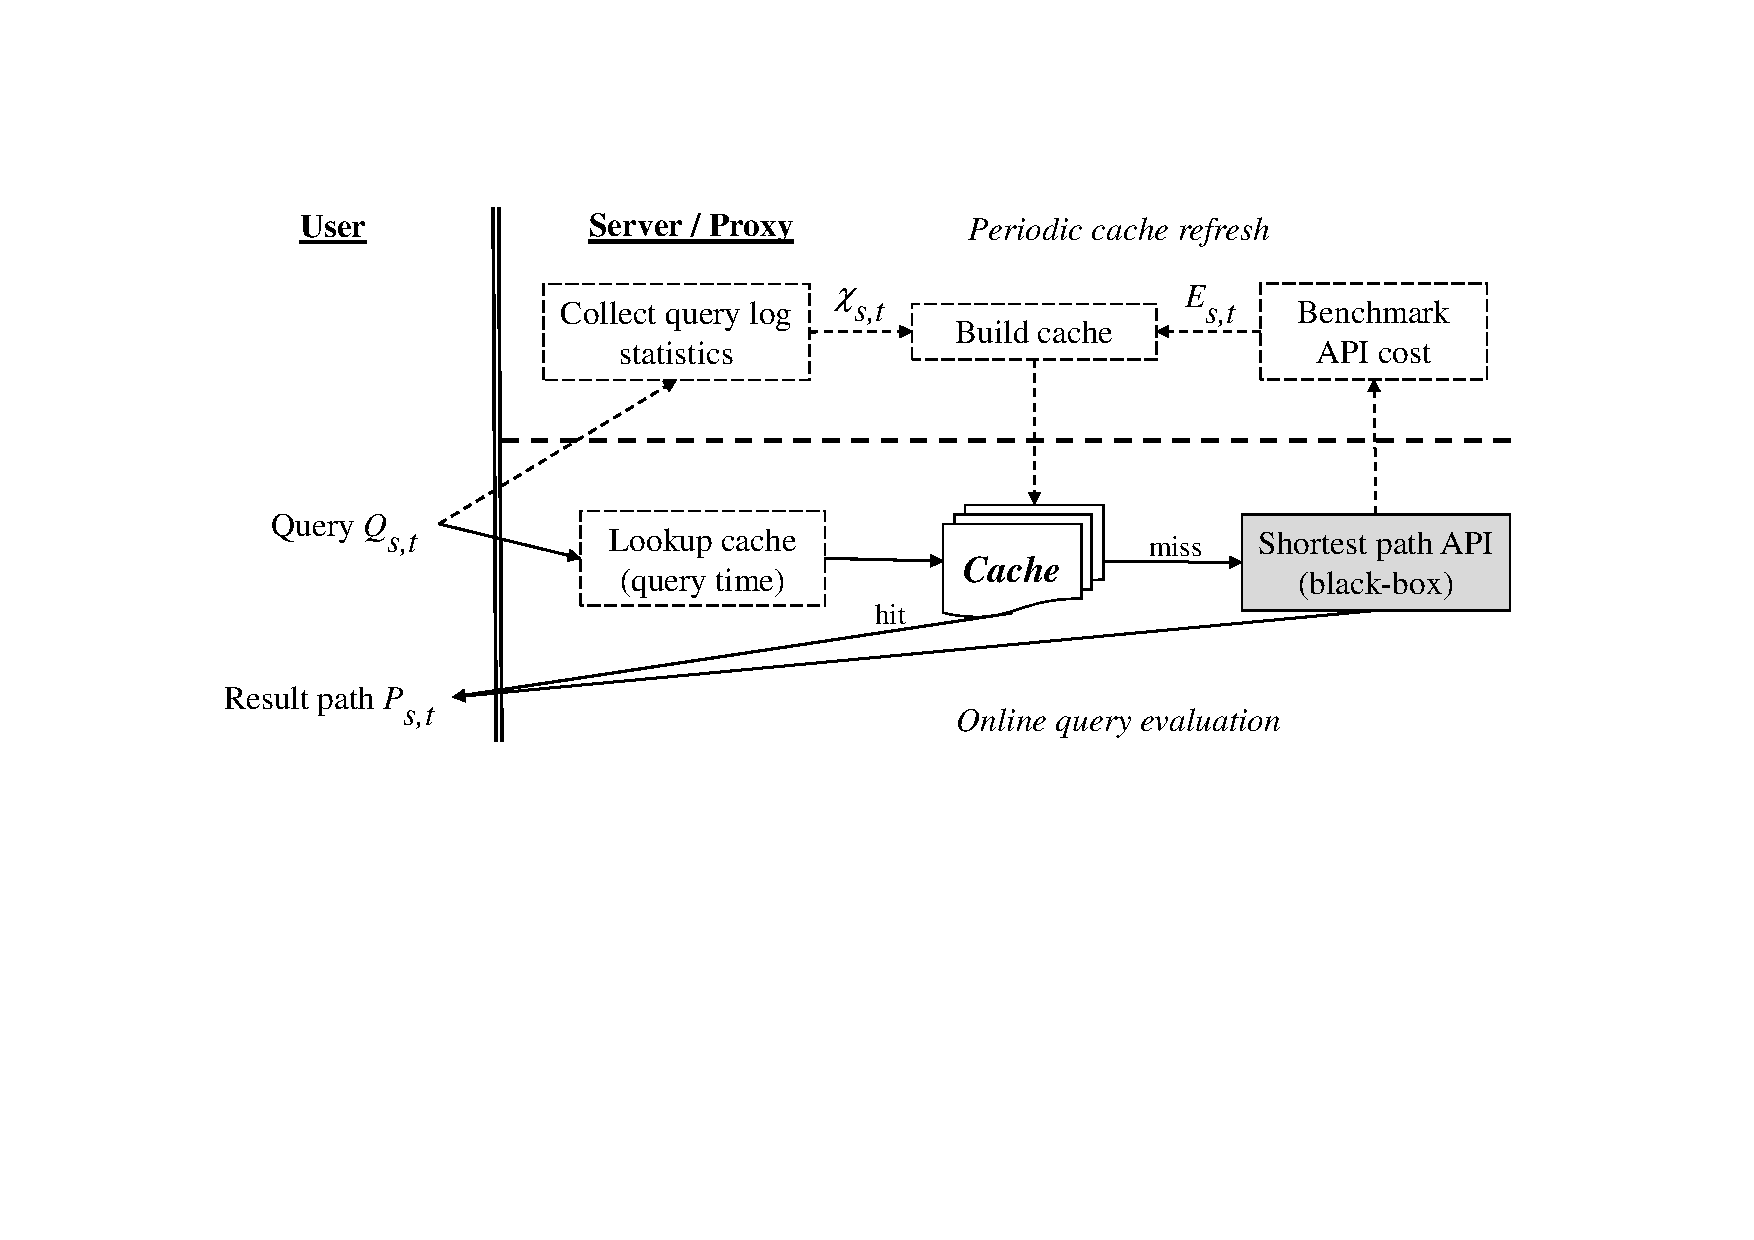
\includegraphics[width=1.0\columnwidth]{figures/routequery}
        \caption{Components in a Static Caching System}
  \label{fig:routequery}
\end{figure}



%number of invocations of shortest calls
%and the total amount of calling time.


% mention the optimization goals here ??
% simply remove the estimation block? (we haven't done it)

% reduce the total cost of invoking it.
% $\Delta T$

% add steps,  Step I, Step II.3., etc.



Unlike web search caching, we observe that
minimizing the cache hit ratio does not necessarily mean that the overall cost is reduced significantly.
In the server scenario, the cost of calling the shortest path API (e.g., shortest path algorithm) is not fixed
and depends heavily on the distance of the shortest path.


As a case study, we randomly generate 500 shortest path queries on two real road networks
(their descriptions are available in Section~\ref{sec:experiments}),
and execute a shortest path algorithm (Dijkstra) for them.
In Figure~\ref{fig:spcost}, each subfigure (for each road network) shows the shortest path distance (x-axis)
and the cost (y-axis) of each individual query.
Observe that there is a strong correlation between the cost and the shortest path distance.
%
Caching a short-range path may only provide a negligible improvement, even if the path is queried frequently.
%On the other hand, caching a long
Therefore, we plan to design a {\em benchmark} for the cost of calling the API.


\begin{figure}[hbt]
  \center
  \begin{tabular}{@{}c@{ }c@{}}
        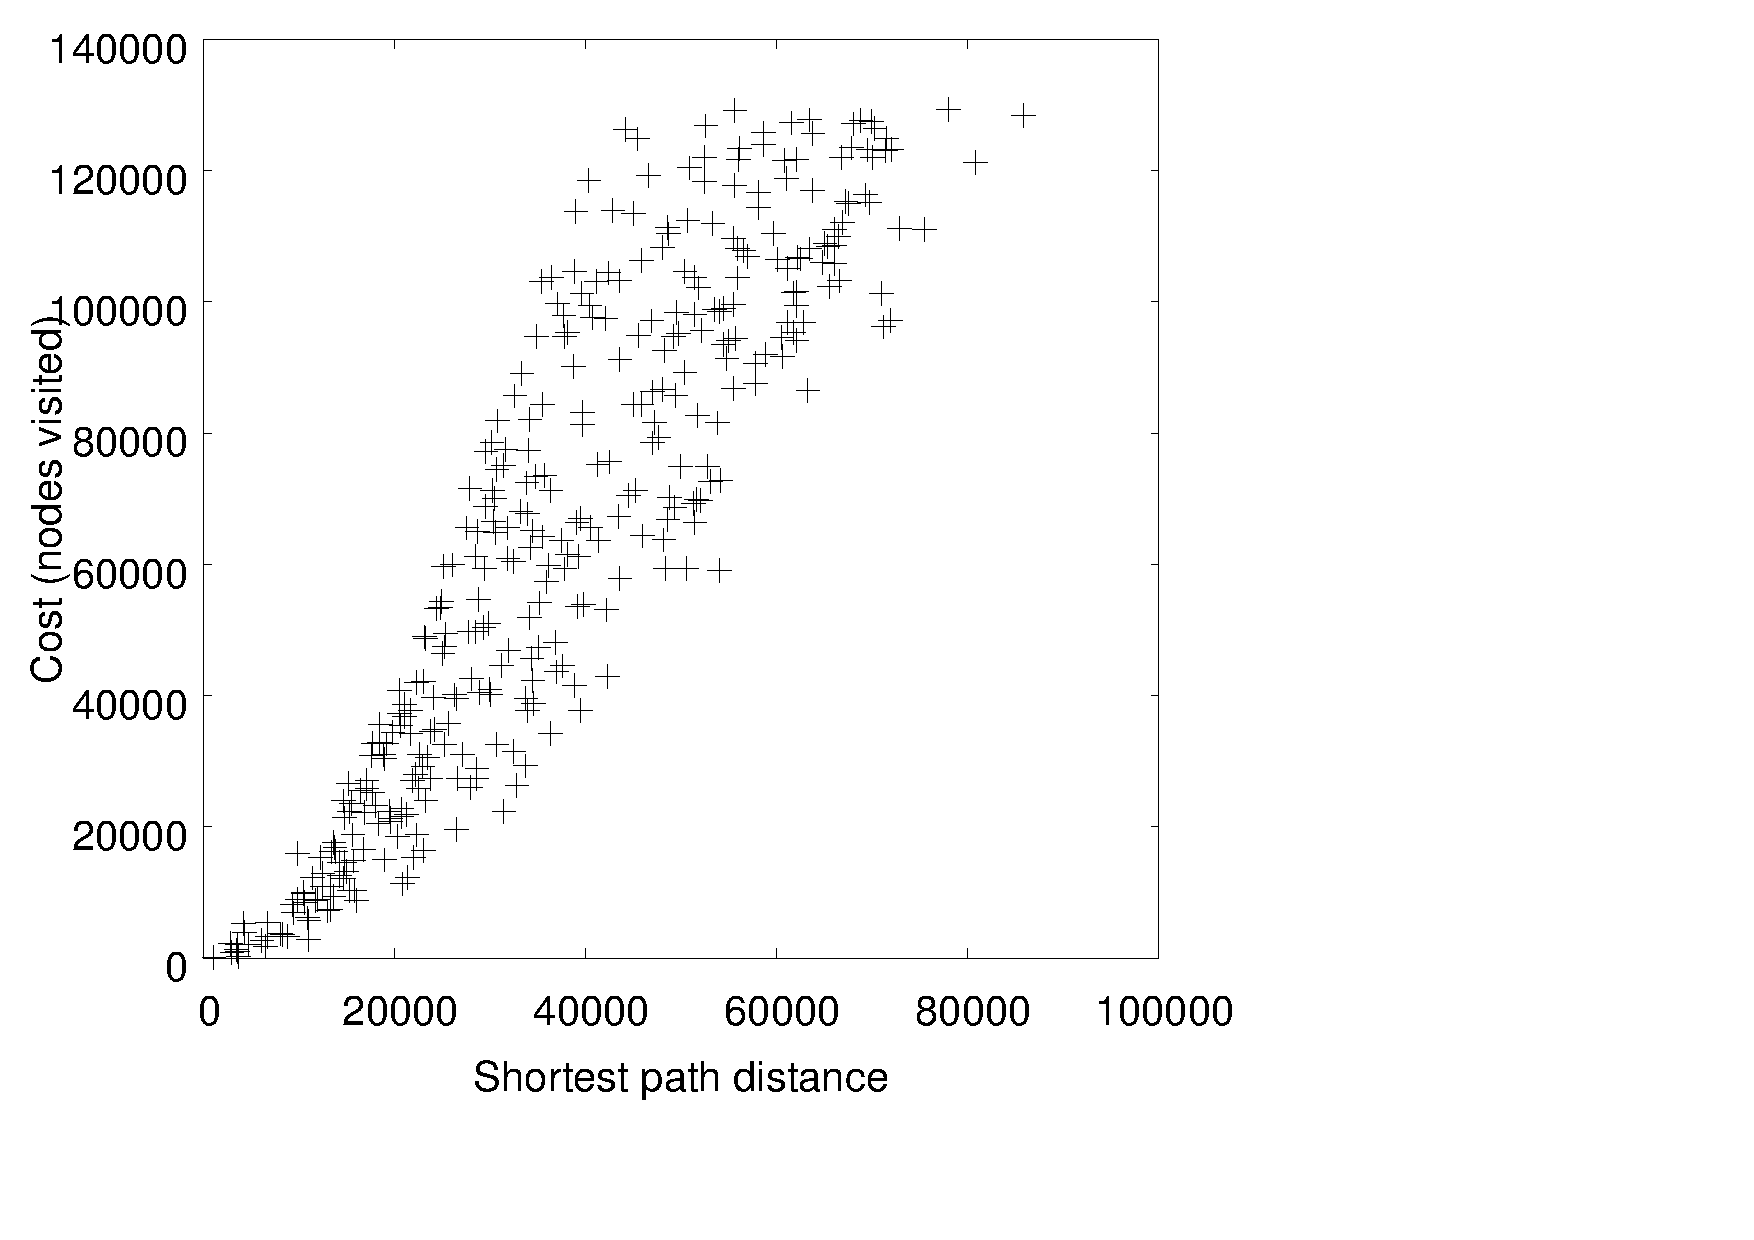
\includegraphics[width=0.5\columnwidth]{figures/AAL_dist}
        &
        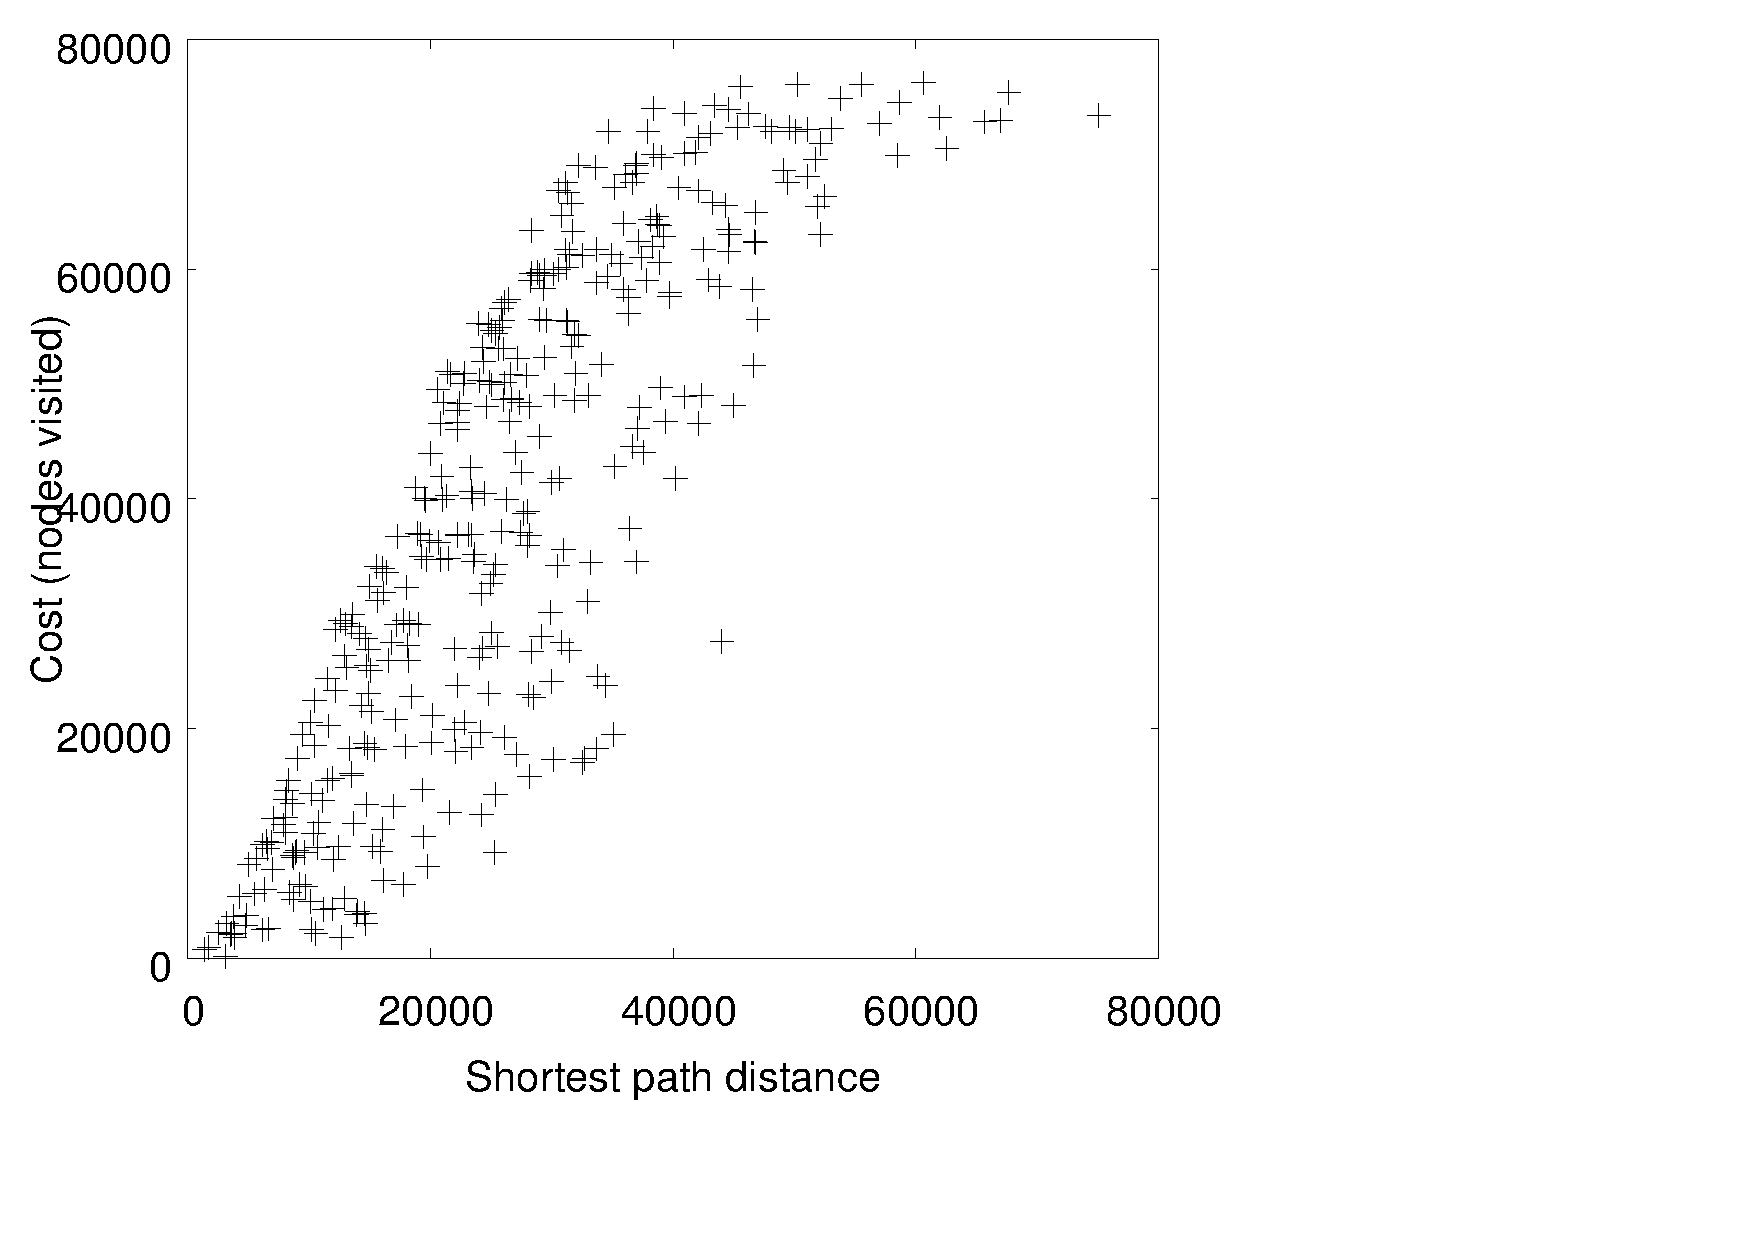
\includegraphics[width=0.5\columnwidth]{figures/BJ_dist}
  \end{tabular}
  \caption{Cost vs. Distance of a Shortest Path Algorithm}
  \label{fig:spcost}
\end{figure}



Adopting the static caching paradigm, the server/proxy {\em collects the query log} and {\em builds the cache}
periodically (e.g., daily).
By extracting the distribution of the query log, we are able to estimate the probability of a specific shortest
path being queried in the future. Combining such information with the benchmark model, we can place
promising paths in the cache in order to minimize the overall cost of the system.
%
We will also investigate the structure of the cache;
it should be compact in order to accommodate as many paths as possible,
and it should support efficient result retrieval.




% overhead


Our main objective is to {\em reduce the overall cost incurred by calling the shortest path API}.
We define this as the problem below.
In Section~\ref{sec:BenefitDriven}, we formulate a cache benefit notion $\gamma(\Psi)$,
extract statistics to compute $\gamma(\Psi)$, and present an algorithm for the cache
benefit maximization problem.

$\\$
\textsc{Problem:} {\bf Static cache benefit maximization problem. $\\$}
%
{\it Given a cache budget $\mathcal{B}$ and a query log $\mathcal{QL}$,
this problem is to build a cache $\Psi$ with the maximum cache benefit $\gamma(\Psi)$ subject to the budget constraint $\mathcal{B}$,
where $\Psi$ contains result paths $P_{s,t}$ whose queries $Q_{s,t}$ belong to $\mathcal{QL}$.
}
$\\$


Our secondary objectives are to: (i) develop a compact cache structure to maximize the accommodation of shortest paths,
and (ii) provide efficient means for retrieving results from the cache.
We will focus on these issues in Section~\ref{sec:CacheStruct}.


%As the main problem with expensive \spath calculations is time needed, we use reduction in \textit{\cet} as the main optimization target and measurement to evaluate our success.
%At a \spath service provider, the time spent to return a \spath result is essentially composed of two tasks: calculating the \spath and the overhead of query processing.



%We want reduce the gross \cet of \spath calculations - goal 1 - as it is the most CPU intensive task at a \spath service, and therefor also the most time consuming. By using a cache we expect to see a negative correlation between cache hit rate and \cet used on \spath calculation.

%In a \spath service there will always be a some overhead associated with \spath query processing. Introducing a cache in front of the existing \spath service (fig. \ref{fig:routequery}B) will undeniably add more overhead as the cache needs to be queried for all queries submitted to the \spath service, regardless of whether it is able to answer the query or not. In order for the cache to be useful, the overhead introduced needs to be minimized (goal \ref{item:goal2}). We always have to make sure that the savings achieved by adding a cache to the system is greater than the overhead introduced.

%The fact that the system will be using a static cache, and \spaths exhibit the \oss property, makes goal 3 - determining the value of a \spath subpath - very important. The ability to do goal \ref{item:goal3} well will have a direct influence on goal \ref{item:goal1} and  \ref{item:goal2}. If we fill the cache with useless \spaths we will end up calculating a \spath for all queries, as well as the overhead from checking the cache for each query. Solving goal 3 well is the most direct way to solve goal 1.



\subsection{Existing Solutions for Caching Results}\label{sec:competitors}
%
We now revisit existing solutions for caching web search results~\cite{Markatos01,BaezaYates03}
and then explain why they are inadequate for shortest path caching.


% We only consider result caching methods

%{\bf ++ try to shrink this section if not enough space}



\stitle{Dynamic Caching---LRU}
%
A typical dynamic caching method for web search is the Least-Recently-Used (LRU) method~\cite{Markatos01}.
%A {\em dynamic caching} method updates the cache content
When a new query is submitted, its result is inserted into the cache.
The least-recently-used result is evicted from the cache when it becomes full.


%Using a dynamic cache and calculating the benefit of each path is very expensive. If a dynamic cache is used, and we want to ensure it always keeps the most useful paths in the cache, it will be very expensive to calculate the benefit of a new query with respect how much it overlaps with existing \spaths (i.e. how many nodes it shares with an existing \spaths) and how likely it will be able to answer a query in the future, thus adding a substantial overhead to query processing. As the benefit of a \spath is so expensive to calculate, while the \spath service is running, it violates goal \ref{item:goal2} in section \ref{subsec:goals}.


We proceed to illustrate the running steps of LRU on the map in Figure~\ref{fig:rxmap}.
Suppose that the cache budget $\mathcal{B}$ is 10 (i.e., it can hold 10 nodes).
Table~\ref{tab:queries} shows the query and the cache content at each time $T_i$.
Each cached path is associated with the last time it was used.
%
At times $T_1$ and $T_2$, both queries produce cache misses and
their results ($P_{3,6}$ and $P_{1,6}$) are inserted into the cache (as they fit).
At time $T_3$, query $Q_{2,7}$ causes a cache miss as it cannot be answered by any cached path.
Before inserting its result $P_{2,7}$ into the cache, the least recently used path $P_{3,6}$ is evicted from the cache.
At time $T_4$, query $Q_{1,4}$ contributes a cache hit;
it can be answered by the cached path $P_{1,6}$ because the source and target nodes $v_1, v_4$ fall on $P_{1,6}$ (see Lemma~\ref{lem:oss}).
%
The running steps at subsequent times are shown in Table~\ref{tab:queries}.
%At time $T_5$, query $Q_{4,8}$ causes a cache miss as it cannot be answered by any cache item.
%Before inserting its result $P_{4,8}$ into the cache, the least recently used cache item $P_{2,7}$ is evicted from the cache.
%%
%At time $T_6$, query $Q_{2,5}$ produces a cache miss. The least recently used cache item $P_{1,6}$ is evicted from the cache
%and then the result of $Q_{2,5}$ is inserted into the cache.
%%
%At time $T_7$, query $Q_{3,6}$ causes a cache miss.
%The least recently used cache item $P_{4,8}$ is evicted from the cache and then the result of $Q_{3,6}$ is inserted into the cache.
%At time $T_8$, query $Q_{3,6}$ leads to a cache hit.
In total, the LRU cache has only 2 hits.

%% mention a better strategy


\begin{table}[hbt]
\center
\begin{tabular}{|@{ }c@{ }|@{ }c@{ }|@{ }c@{ }||@{ }c@{ }|@{ }c@{ }|}\hline
    Time	&	$Q_{s,t}$	& $P_{s,t}$ &  Paths in LRU cache & event  \\\hline
    $T_1$	&	$Q_{3,6}$ 	& $\langle v_3,v_4,v_5,v_6 \rangle$ & $P_{3,6}:T_1$ & miss  \\
    $T_2$	&	$Q_{1,6}$ 	& $\langle v_1,v_3,v_4,v_5,v_6 \rangle$ & $P_{1,6}:T_2, \;\; P_{3,6}:T_1$ & miss \\
    $T_3$	&	$Q_{2,7}$ 	& $\langle v_2,v_3,v_4,v_5,v_7 \rangle$ & $P_{2,7}:T_3, \;\; P_{1,6}:T_2$ & miss \\
    $T_4$	&	$Q_{1,4}$ 	& $\langle v_1,v_3,v_4 \rangle$ & $P_{1,6}:T_4, \;\; P_{2,7}:T_3$ & hit \\
    $T_5$	&	$Q_{4,8}$ 	& $\langle v_4,v_5,v_7,v_8 \rangle$ & $P_{4,8}:T_5, \;\; P_{1,6}:T_4$ & miss \\
    $T_6$	&	$Q_{2,5}$ 	& $\langle v_2,v_3,v_4,v_5 \rangle$ & $P_{2,5}:T_6, \;\; P_{4,8}:T_5$ & miss \\
    $T_7$	&	$Q_{3,6}$ 	& $\langle v_3,v_4,v_5,v_6 \rangle$ & $P_{3,6}:T_7, \;\; P_{2,5}:T_6$ & miss \\
    $T_8$	&	$Q_{3,6}$ 	& $\langle v_3,v_4,v_5,v_6 \rangle$ & $P_{3,6}:T_8, \;\; P_{2,5}:T_6$ & hit \\\hline
\end{tabular}
\caption{Example of LRU on a Sequence of Queries}
\label{tab:queries}
\end{table}


%However, LRU suffers from the following drawbacks:

Observe that LRU cannot determine the benefit of a path effectively.
For example, paths $P_{1,6}$ and $P_{2,7}$ (obtained at times $T_2$ and $T_3$)
can answer many queries at subsequent times, e.g., $Q_{1,4}, Q_{2,5}, Q_{3,6}, Q_{3,6}$.
If they were kept in the cache, there would be 4 cache hits.
However, LRU evicts them before they can be used to answer other queries.


Another limitation of LRU is that it is not designed to support subpath matching efficiently.
Upon receiving a query $Q_{s,t}$, every path in the cache needs to be scanned in order to check whether the path
contains $s$ and $t$. This incurs significant runtime overhead, outweighing the advantages of the cache.



%makes local decisions and
%Because LRU does not have a scoring function then, even if a path $SP$ is valuable (covers many potential queries), if a sequence of consecutive queries, which $SP$ can not cover, is submitted, then P will be evicted.
%not sufficient time to collect the frequency?  (local decision only)
%The end result is that 30\% of the cache space is wasted and out of the 6 queries only we only resulted in a 1 cache hit.






\stitle{Static Caching---HQF}
%
A typical static caching method for web search is the Highest-Query-Frequency (HQF) method~\cite{BaezaYates03}.
In an offline phase, the most frequent queries are selected from the query log $\mathcal{QL}$,
and then their results are inserted into the cache.
The cache content remains unchanged during runtime.


According to Ref.~\cite{BaezaYates03},
the frequency of a query is counted as the number of queries in $\mathcal{QL}$ that are identical to it.
Let us consider an example query log: $\mathcal{QL}=\{ Q_{3,6}, Q_{1,6}, Q_{2,7}, Q_{1,4}, Q_{4,8}, Q_{2,5}, Q_{3,6}, Q_{3,6} \}$.
Since $Q_{3,6}$ has the highest frequency (3), HQF picks the corresponding result path $P_{3,6}$.
It fails to pick $P_{1,6}$ simply because its query $Q_{1,6}$ has a low frequency (1).
In fact, the path $P_{1,6}$ is more promising than $P_{3,6}$ because
$P_{1,6}$ can be used to answer more queries than $P_{3,6}$.
%Thus, HQF is unable to pick promising paths (e.g., the results of $Q_{1,6}$ and $Q_{2,7}$).
%Due to ties, HQF may pick  into the cache.
This creates a problem in HQF because the query frequency definition does not
capture characteristics specific to our problem---shortest paths may overlap,
and the result of a query may be used to answer multiple other queries.


% (i.e., queries in Table~\ref{tab:queries}).
% maybe we need to consider approaches that put the most frequent query into the cache



\stitle{Other common limitations of LRU and HQF}
%
Furthermore, neither LRU nor HQF consider
the variations in the expense of obtaining shortest paths.
Consider the cache in the server scenario as an example.
Intuitively, it is more expensive to process a long-range query than a short-range query.
Caching an expensive-to-obtain path could lead to greater savings in the future.
An appropriate choice of cached path should take such expenses into account.

Also, they have not studied the utilization of the cache space for shortest paths.
For example, in Table~\ref{tab:queries}, the paths in the cache overlap
and cause wasted space on storing duplicate nodes among the paths.
It is important to design a compact cache structure that exploits the sharing among paths
to avoid storing duplicated nodes.


%Q1 and Q2 are identical except for one node, which waste a lot of space on . Had we represented each node only once, we would be able to fit all nodes in the map in the cache.







\section{Benefit-Driven Caching} \label{sec:BenefitDriven}
%
In this section, we propose a benefit-driven approach to decide which shortest paths
should be placed in the cache.
Section~\ref{sec:BenefitModel} formulates a systematic model for capturing the {\em benefit} of a cache
%shortest path
on potential queries. This model requires the knowledge of:
(i) the frequency $\chi_{s,t}$ of a query, and (ii) the expense $E_{s,t}$ of processing a query.
%
Thus, we investigate how to extract query frequencies from a query log in Section~\ref{sec:extract}
and benchmark the expense of processing a query in Section~\ref{sec:benchmark}.
Finally, in Section~\ref{sec:greedy}, we present an algorithm for selecting promising paths to be placed in the cache.


%explain what will be introduced, which sub-problems are considered, and which subsections presents what.
%
%(i) estimating the benefit of a shortest path based on its query probability and cost saving,
%and (ii) applying a greedy approach


% Intro to section
% Show benefits of a static cache over a dynamic cache
% List all advantages of a static cache solution
% Static cache has no maintenance cost after filling the cache



% <to be presented in a bullet form rather than an algorithm>
%\begin{figure}[bht]
%  \center
%        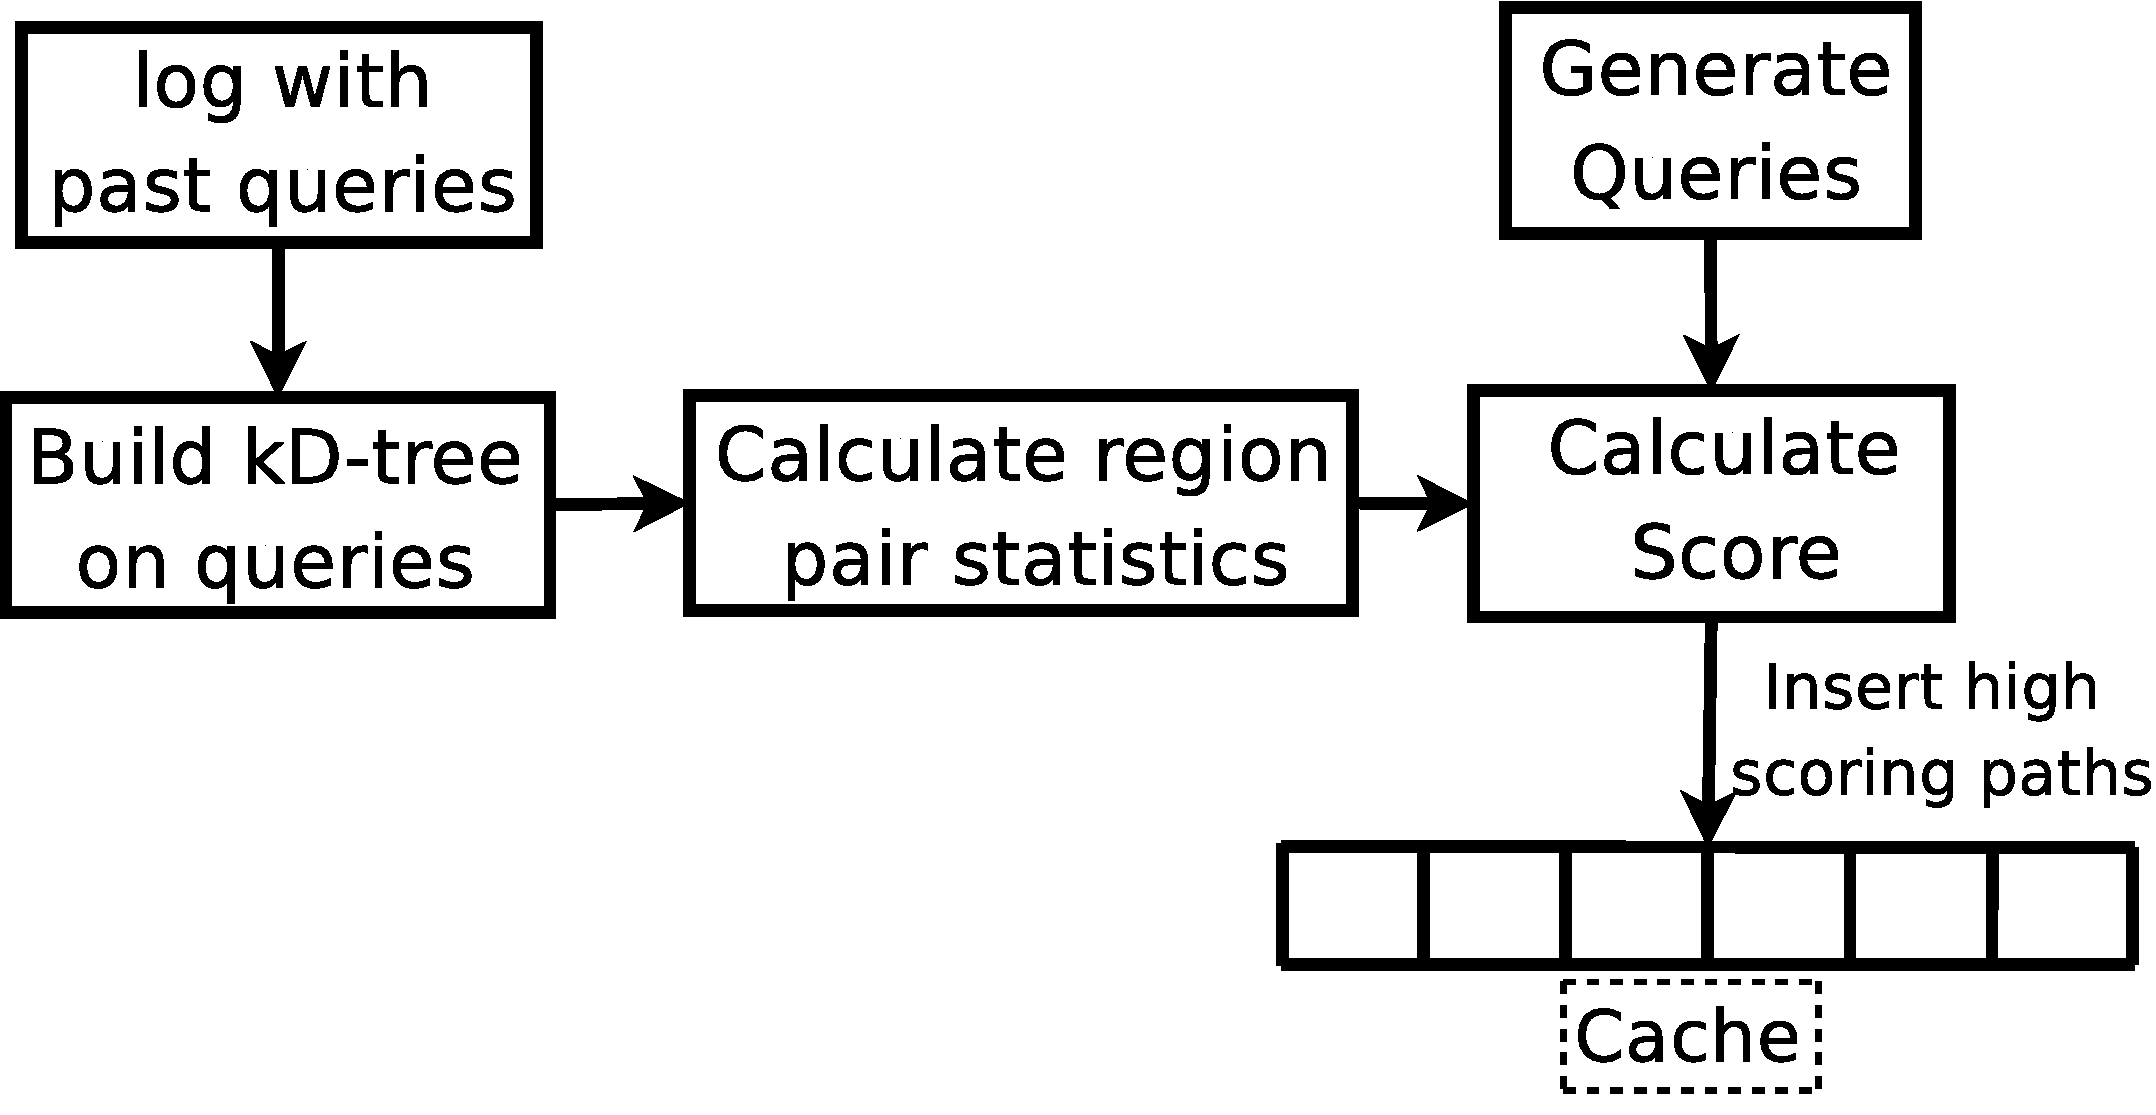
\includegraphics[width=0.5\textwidth]{figures/fillcache}
%        \caption{Insertion of cache elements in offline phase.}
%  \label{fig:fillcache}
%\end{figure}


\subsection{Benefit Model}\label{sec:BenefitModel}
%
%This section presents a benefit model of a cache on shortest path queries.
We first study the benefit of a cached shortest path
and then examine the benefit of a cache.


First, we consider a cache $\Psi$ that contains one shortest path $P_{a,b}$ only.
Recall from Figure~\ref{fig:routequery} that,
when a query $Q_{s,t}$ can be answered by a cached path $P_{a,b}$,
this produces a cache hit and avoids the cost of invoking the shortest path API.
% Otherwise, the result must be obtained by calling ......
% this is the benefit of a path
In order to model the benefit of $P_{a,b}$, we must address the questions below:
\begin{enumerate}
    \itemsep -2pt
    \item Which queries $Q_{s,t}$ can be answered by the path $P_{a,b}$?
    \item For query $Q_{s,t}$, how much cost can we save?
\end{enumerate}
% queries can be answered



The first question is answered by Lemma~\ref{lem:oss}.
The path $P_{a,b}$ contains the path $P_{s,t}$ when both nodes $v_s$ and $v_t$ appear in $P_{a,b}$.
Thus, we define the {\em answerable query set} of the path $P_{a,b}$ as:
\begin{equation} \label{eq:phi}
 \mathfrak{U} (  P_{a,b} ) = \{ P_{s,t} : s \in P_{a,b}, t \in P_{a,b}, s \neq t \}
\end{equation}
% \Cup \mathbb{U}
It contains the set of queries that can be answered by $P_{a,b}$.
Taking Figure~\ref{fig:rxmap} as the example graph, the answerable query set
of path $P_{1,6}$ is: $\mathfrak{U} (  P_{1,6} ) = \{ P_{1,3},P_{1,4},P_{1,5},P_{1,6}$,
$P_{3,4},P_{3,5},P_{3,6}$, $P_{4,5},P_{4,6},P_{5,6} \}$.
Table~\ref{tbl:subpath} shows the answerable query sets of other paths.



\begin{table}
\center
    \begin{tabular}{|@{ }c@{ }|@{ }c@{ }|}
        \hline
        $P_{a,b}$           &  $\mathfrak{U}(P_{a,b})$ \\ \hline
        $P_{1,4}$      	    & $P_{1,3},P_{1,4},P_{3,4}$ \\
        $P_{1,6}$  	        & $P_{1,3},P_{1,4},P_{1,5},P_{1,6},P_{3,4},P_{3,5},P_{3,6},P_{4,5},P_{4,6},P_{5,6}$\\
        $P_{2,5}$   	    & $P_{2,3},P_{2,4},P_{2,5},P_{3,4},P_{3,5},P_{4,5}$ \\
        $P_{2,7}$      	    & $P_{2,3},P_{2,4},P_{2,5},P_{2,7},P_{3,4},P_{3,5},P_{3,7},P_{4,5},P_{4,7},P_{5,7}$ \\
        $P_{3,6}$       	& $P_{3,4},P_{3,5},P_{3,6},P_{4,5},P_{4,6},P_{5,6}$ \\
        $P_{4,8}$       	& $P_{4,5},P_{4,7},P_{4,8},P_{5,7},P_{5,8},P_{7,8}$ \\ \hline
    \end{tabular}
    \begin{tabular}{|c|}
        \hline
        $\mathfrak{U}(\Psi)$, when $\Psi = \{P_{1,6},P_{3,6}\}$ \\ \hline
        $P_{1,3},P_{1,4},P_{1,5},P_{1,6},P_{3,4},P_{3,5},P_{3,6},P_{4,5},P_{4,6},P_{5,6}$ \\ \hline
    \end{tabular}
    \caption{Example of $\mathfrak{U}(P_{s,t})$ and $\mathfrak{U}(\Psi)$}
\label{tbl:subpath}
\end{table}


Regarding the second question, the expected cost savings for query $Q_{s,t}$ depends on
(i) its query frequency $\chi_{s,t}$ and (ii) the expense $E_{s,t}$ for the shortest path API to process it.
%Intuitively, an expensive path (high $E_{s,t}$) or a frequent query (high $\chi_{s,t}$)
Since the path $P_{a,b}$ can answer query $Q_{s,t}$,
we save cost $E_{s,t}$ a total of $\chi_{s,t}$ times, i.e., $\chi_{s,t} \cdot E_{s,t}$ in total.%
\footnote{We ignore the overhead of cache lookup as it is negligible compared to the expense $E_{s,t}$ of processing a query $Q_{s,t}$.
Efficient cache structures are studied in Section~\ref{sec:CacheStruct}.}


Combining the answers to both questions, we define the {\em benefit} of path $P_{a,b}$ as:
\begin{equation} \label{eq:benefitPath}
\gamma(P_{a,b}) = \sum_{P_{s,t} \in \mathfrak{U}(P_{a,b})} \chi_{s,t} \cdot E_{s,t}
\end{equation}
The path benefit $\gamma(P_{a,b})$ answers the question: {\em ``If path $P_{a,b}$ is in the cache, how much cost can we save in total?''}




Let us assume that we are given the values of $\chi_{s,t}$ and $E_{s,t}$ for all pairs of $v_s$ and $v_t$,
as shown in Figure~\ref{fig:freqcost}.
We study how to derive them in subsequent sections.
%
To compute $\gamma(P_{1,6})$ of path $P_{1,6}$, we first find its answerable query set $\mathfrak{U}(P_{1,6})$ (see Table~\ref{tbl:subpath}).
Since $\mathfrak{U}(P_{1,6})$ contains the path $P_{1,4}$, it contributes a benefit of
$\chi_{1,4} \cdot E_{1,4} = 1 \cdot 2$ (by lookup in Figure~\ref{fig:freqcost}).
Summing up the benefits of all paths in $\mathfrak{U}(P_{1,6})$, we thus obtain:
$\gamma(P_{1,6})=0+1\cdot2+0+1\cdot4+0+0+3\cdot3+0+0+0=15$.
Similarly, we can compute the benefit of path $P_{3,6}$:
$\gamma(P_{3,6})=0+0+3\cdot3+0+0+0=9$.




We then extend our equations to the general case---a cache with multiple shortest paths.
Observe that a query can be answered by the cache $\Psi$ if it can be answered
by any path $P_{a,b}$ in $\Psi$.
Thus, we define the answerable query set of $\Psi$ as the union of all $\mathfrak{U}( P_{a,b} )$,
and define the benefit of $\Psi$ accordingly.
\begin{eqnarray} \label{eq:upsi}
 \mathfrak{U}(\Psi) & = &  \bigcup_{ P_{a,b} \in \Psi} \mathfrak{U}( P_{a,b} ) \\
 %
 \label{eq:benefitCache}
 \gamma(\Psi) &  = &  \sum_{P_{s,t} \in \mathfrak{U}(\Psi)} \chi_{s,t} \cdot E_{s,t}
\end{eqnarray}
The cache benefit $\gamma(\Psi)$ answers the question: {\em ``Using this cache $\Psi$, how much cost can we save in total?''}


Suppose that the cache $\Psi$ contains two paths $P_{1,6}$ and $P_{3,6}$.
The answerable query set $\mathfrak{U}(\Psi)$ of $\Psi$ is shown in Table~\ref{tbl:subpath}.
By Equation~\ref{eq:benefitCache}, we compute the cache benefit as:
$\gamma(\Psi) = 1\cdot2 + 1\cdot4 + 3\cdot3 = 15$.


%    cannot simply sum
Note that $\gamma(\Psi)$ is not a distributive function.
For example, $\gamma(P_{1,6}) + \gamma(P_{3,6}) = 15 + 9 = 24 \ne \gamma(\Psi)$.
%
Since the path $P_{3,6}$ appears in both answerable query sets,
$\mathfrak{U}(P_{1,6})$ and $\mathfrak{U}(P_{3,6})$,
the benefit contributed by $P_{3,6}$ is double-counted in the sum $\gamma(P_{1,6}) + \gamma(P_{3,6})$.
%
On the other hand, the value of $\gamma(\Psi)$ is correct because
the path $P_{3,6}$ appears exactly once in the answerable query set $\mathfrak{U}(\Psi)$ of the cache.


%its contributing benefit $\chi_{3,6} \cdot E_{3,6} = 3$ to the cache is counted once.



\stitle{Benefit per size}
%
The benefit model does not consider the size $|P_{a,b}|$ of a path $P_{a,b}$ into account.
%
Suppose that we are given two paths $P_{a,b}$ and $P_{a',b'}$
such that they have the same benefit (i.e., $\gamma(P_{a,b})=\gamma(P_{a',b'})$)
and $P_{a',b'}$ has a smaller size than $P_{a,b}$.
%
Intuitively, we prefer path $P_{a',b'}$ rather than path $P_{a,b}$
because $P_{a',b'}$ occupies less space, leaving more cache space for placing other paths.
Thus, we define the {\em benefit-per-size} of a path $P_{a,b}$ as:
\begin{eqnarray} \label{eq:benefitPerSize}
\overline{\gamma}(P_{a,b}) & = & \frac{  \gamma(P_{a,b}) }{  |P_{a,b}| }
\end{eqnarray}
We will utilize this notion in Section~\ref{sec:greedy}.


%{\bf Benefit per size. $\\$}





Recall from Section~\ref{subsec:goals} that
our main problem is to build a cache $\Psi$ such that its benefit $\gamma(\Psi)$ is maximized.
This requires values for $\chi_{s,t}$ and $E_{s,t}$.
We discuss how to obtain these values in subsequent sections.





%++ discuss tasks to be done next, (i) estimation, (ii) Our method attempts to maximize




%$P_{3,6}$  counted once ...
% the effect of covering paths ...


%We will define our goals formally, introducing the benefit equations we aim to minimize.
%
%
%
%A query is a pair of nodes ids $(v_s, v_t)$, denoted $Q_{s,t}$ and the \spath returned from such query we denote $Q_{s,t}$.
%In order to evaluate goal \ref{item:goal3} we calculate the benefit of the content in the cache, denoted $\gamma(\Psi)$. To calculate $\gamma(\Psi)$ we find the set of unique subpaths from all \spaths in the cache ($\Psi$) and sum up the frequency, $\chi_{s,t}$, of each unique path.
%$\chi$, a table of benefit computed from existing historical data (query log). An example of different entries, $\chi_{s,t}$, is given in table \ref{tab:freq}





\begin{figure}[hbt]
    \center
    \begin{tabular}{@{}cc@{}}
        \begin{tabular}{|@{ }c@{ }|@{ }c@{ }c@{ }c@{ }c@{ }c@{ }c@{ }c@{ }c@{ }|}
            \hline
            $\chi_{s,t}$	& $v_1$	& $v_2$	& $v_3$	& $v_4$	& $v_5$	& $v_6$	& $v_7$ & $v_8$ \\\hline
            $v_1$			& /	& 0	& 0	& 1	& 0	& 1	& 0	& 0	 \\
            $v_2$			& 0	& /	& 0	& 0	& 1	& 0	& 1	& 0	 \\
            $v_3$			& 0	& 0	& /	& 0	& 0	& 3	& 0	& 0	 \\
            $v_4$			& 1	& 0	& 0	& /	& 0	& 0	& 0	& 1	 \\
            $v_5$			& 0	& 1	& 0	& 0	& /	& 0	& 0	& 0	 \\
            $v_6$			& 1	& 0	& 3	& 0	& 0	& /	& 0	& 0	 \\
            $v_7$			& 0	& 1	& 0	& 0	& 0	& 0	& / & 0  \\
            $v_8$			& 0	& 0	& 0	& 1	& 0	& 0	& 0 & /  \\
            \hline
        \end{tabular}
        &
        \begin{tabular}{|@{ }c@{ }|@{ }c@{ }c@{ }c@{ }c@{ }c@{ }c@{ }c@{ }c@{ }|}
            \hline
            $E_{s,t}$	& $v_1$	& $v_2$	& $v_3$	& $v_4$	& $v_5$	& $v_6$	& $v_7$	& $v_8$ \\\hline
            $v_1$			& /	& 2	& 1 & 2	& 3	& 4	& 4	& 5   \\
            $v_2$			& 2	& /	& 1	& 2	& 3	& 4	& 4	& 5   \\
            $v_3$			& 1	& 1	& /	& 1	& 2	& 3	& 3	& 4   \\
            $v_4$			& 2	& 2	& 1	& /	& 1	& 2	& 2	& 3   \\
            $v_5$			& 3	& 3	& 2	& 1	& /	& 1	& 1	& 2   \\
            $v_6$			& 4	& 4	& 3	& 2	& 1	& /	& 2	& 3   \\
            $v_7$			& 4	& 4	& 3	& 2	& 1	& 2	& /	& 1   \\
            $v_8$			& 5	& 5	& 4	& 3	& 2	& 3	& 1	& /   \\
            \hline
        \end{tabular} \\
        (a) $\chi_{s,t}$ values & (b) $E_{s,t}$ values
    \end{tabular}
    \caption{Example of $\chi_{s,t}$ and $E_{s,t}$ values for the graph}
\label{fig:freqcost}
\end{figure}





%When we want to evaluate the benefit of $\Psi$ we first calculate $\mathfrak{U}(\spath)$ for each \spaths. Table \ref{tab:chi} shows the set of subpaths from the \spaths for each query Q1-Q6 from table \ref{tab:queries} (we assume all queries fit into the cache). Once we have all the sets of subpaths from the cache content, we use equation \ref{eq:upsi} to union them together and obtain the set of unique subpaths in the cache, $\mathfrak{U}(\Psi)$ (see table \ref{tab:chi}). After we have obtained $\mathfrak{U}(\Psi)$, we use equation \ref{eq:benefit} to calculate $\gamma(\Psi)$, the total benefit we expect to have with the content in $\Psi$. With $\mathfrak{U}(\Psi)$ obtained, using $\chi_{s,t}$ values from table \ref{tab:freq}, $\gamma(\Psi)$ would be 6 i.e. $\chi_{1,6}+\chi_{2,6}+\chi_{1,4}+\dotsb+\chi_{3,6} = 6$, finding a value in table \ref{tab:freq} for all \spaths of $\mathfrak{U}(\Psi)$ (Tab. \ref{tab:chi}).
%
%Potential \spath$_{s,t}$ items are scored based the $\chi_{s,t}$-value found using the \spath start and end nodes. The score will be zero if the path is already covered by a path, or subpath, already present in the cache. If we assume $P_{1,6}$ (Q1) is already in the cache and we are considering to insert either $P_{2,6}$(Q2) or $P_{4,8}$(Q4) next, then we first find the entry in table \ref{tab:freq} for each query, and check neither is already covered by the content of $\Psi$, i.e not covered by Q1. The score of Q2 would be 2 and for Q4 it would be 1. In this case we would then insert Q2 as it represents the largest expected benefit if inserted into $\Psi$.




% *****************************************
%\subsection{Hardness Analysis}
%Theoretical analysis showing how hard the problem is to solve for \spath caching.\\
%show it is NP-Hard





\subsection{Extracting {\Large $\chi_{s,t}$} from Query Log}\label{sec:extract}
%
%Make clear about the input $\mathcal{QL}$ and output $\chi_{s,t}$
The frequency $\chi_{s,t}$ of query $Q_{s,t}$ plays an important role in our benefit model.
According to a scientific study~\cite{nature}, the mobility patterns of human users follow a
skewed distribution.
% Thus, we expect that different $Q_{s,t}$ have different $\chi_{s,t}$.
For instance, hot regions (e.g., shopping malls, residential buildings) are expected to have high $\chi_{s,t}$,
whereas rural regions are likely to have low $\chi_{s,t}$.
%The values of $\chi_{s,t}$ may be specified by the system administrator in advance;
%however, it requires domain-specific knowledge.


In this section, we propose automatic techniques for deriving the values of $\chi_{s,t}$.
In our caching system (see Figure~\ref{fig:routequery}), the server/proxy
periodically collects the query log $\mathcal{QL}$ and extracts the values of $\chi_{s,t}$.
The literature on static web caching~\cite{BaezaYates07} suggests that the query frequency is stable within a month
and that a month can be used as the periodic time interval.
% based on the assumption: future workload is expected to be similar to the query log
We first study a simple method to extract $\chi_{s,t}$,
and then propose a more effective method for extracting $\chi_{s,t}$.


% more evidence from the workload-aware branch

%  why not uniform distribution (not needed now)
%A naive way is to set uniform distribution of all possible queries ($\chi_{s,t} = 1$), meaning that the \spaths chosen will be evenly distributed over the entire map.
% unable to capture distribution












\begin{table}[hbt]
\center
    \begin{tabular}{|c|@{ }c@{ }c@{ }c@{ }c@{ }c@{ }c@{ }c@{ }c@{ }|}
    \hline
    Timestamp & $T_1$ & $T_2$ & $T_3$ & $T_4$ & $T_5$ & $T_6$ & $T_7$ & $T_8$  \\ \hline
    Query  & $Q_{3,6}$ & $Q_{1,6}$ & $Q_{2,7}$  & $Q_{1,4}$  & $Q_{4,8}$  & $Q_{2,5}$  & $Q_{3,6}$  & $Q_{3,6}$ \\ \hline
    \end{tabular}
\caption{Query log $\mathcal{QL}$}
\label{tbl:querylog}
\end{table}



%  basic filling  O(|V|^2) space
%\stitle{All-pairs frequency table of $\chi_{s,t}$}
\stitle{Node-pair frequency counting}
%
%  The query log $\mathcal{QL}$ may have a huge size  (can be a week point)
In this method, we first create a {\em node-pair frequency table}
$\chi$ with $|V| \times |V|$ entries, like the one in Figure~\ref{fig:freqcost}a.
The entry in the $s$-th row and the $t$-th column represents the value of $\chi_{s,t}$.
The storage space of the table is $O(|V|^2)$, regardless of how large the query log is.

At the beginning, all entries in the table are initialized to zero.
Next, we examine each query $Q_{s,t}$ in the query log $\mathcal{QL}$
and increment the entry $\chi_{s,t}$ (and $\chi_{t,s}$).
% example
Consider the query log $\mathcal{QL}$ in Table~\ref{tbl:querylog} as an example.
For the first query $Q_{3,6}$ in $\mathcal{QL}$, we increment the entries $\chi_{3,6}$ and $\chi_{6,3}$.
Continuing this process with the other queries in $\mathcal{QL}$,
we obtain the table $\chi$ shown in Figure~\ref{fig:freqcost}a.
The $\chi_{s,t}$ values in the table $\chi$ can then be readily used by our benefit model in Section~\ref{sec:BenefitModel}.



% space consumption (not feasible)

% stored in a map (to save space)
% sparse

% but worst case ...




%  partitioning histogram   O(F^2) space
%\stitle{Region-pairs frequency table of $\widehat{\chi}_{R_i,R_j}$}
\stitle{Region-pair frequency counting}
%
The node-pair frequency table $\chi$ requires $O(|V|^2)$ space,
which cannot fit into main memory even for a road network of moderate size (e.g., $|V|=100,000$).
% define what is $\widehat{\chi}_{R_i,R_j}$
To tackle this issue, we propose to: (i) partition the graph into $L$ regions (where $L$ is system parameter),
and (ii) employ a compact table for storing the query frequency among pairs of regions only.
%As we will discuss shortly, the parameter $L$


For the first step, we can apply any existing graph partitioning technique (e.g., kD-tree partitioning, spectral partitioning).
The kD-tree partitioning is applicable to the majority of road networks whose nodes are associated with coordinates.
For other graphs, we may apply spectral partitioning, which does not require node coordinates.
In Figure~\ref{fig:mappartition}, we apply a kD-tree on the coordinates of nodes
in order to partition the graph into $L=4$ regions: $R_1, R_2, R_3, R_4$.




For the second step, we create a {\em region-pair frequency table} $\widehat{\chi}$ with $L \times L$ entries,
like the one in Figure~\ref{fig:regionfreq}b.
The entry in the $R_i$-th row and the $R_j$-th column represents the value of $\widehat{\chi}_{R_i,R_j}$.
The storage space of this table is only $O(L^2)$ and it can be controlled by the parameter $L$.
Initially, all entries in the table are set to zero.
For each query $Q_{s,t}$ in the query log $\mathcal{QL}$,
we first find the region (say, $R_i$) that contains node $v_s$ and
the region (say, $R_j$) that contains node $v_t$.
Then we increment the entry $\widehat{\chi}_{R_i,R_j}$ and $\widehat{\chi}_{R_j,R_i}$.
As an example, we read the query log $\mathcal{QL}$ in Table~\ref{tbl:querylog}
and examine the first query $Q_{3,6}$.
We find that nodes $v_3$ and $v_6$ fall in the regions $R_2$ and $R_3$, respectively.
Thus, we increment the entries $\widehat{\chi}_{R_2,R_3}$ and $\widehat{\chi}_{R_3,R_2}$.
Continuing this process with the other queries in $\mathcal{QL}$,
we obtain the table $\widehat{\chi}$ as shown in Figure~\ref{fig:regionfreq}b.

\begin{figure}[htb]
  \center
        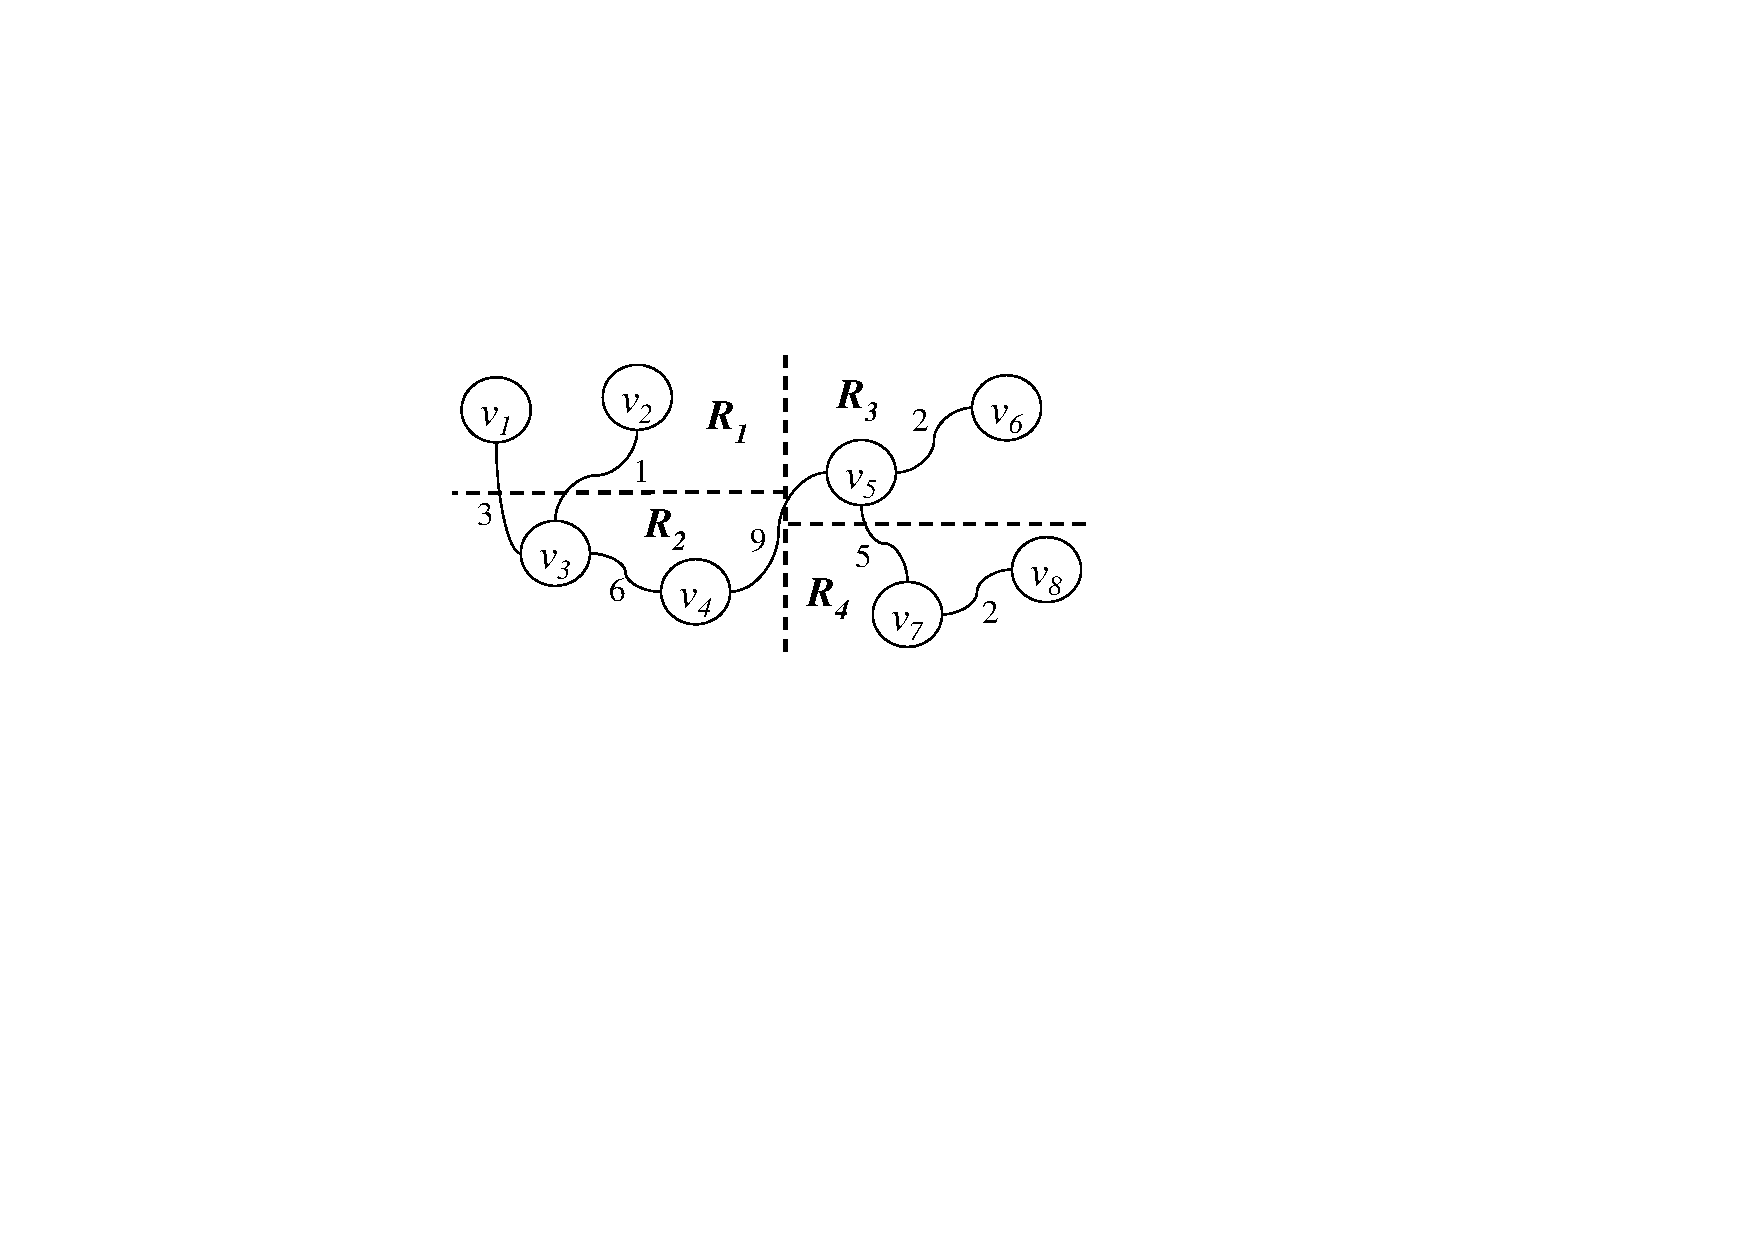
\includegraphics[width=0.7\columnwidth]{figures/mappartition}
        \caption{A graph partitioned into 4 regions}
  \label{fig:mappartition}
\end{figure}
\begin{figure}[htb]
\center
\begin{tabular}{cc}
    \begin{tabular}{cc}
    $R_1 :$ 	& $\{v_1,v_2\}$\\
    $R_2 :$ 	& $\{v_3,v_4\}$ \\
    $R_3 :$ 	& $\{v_5,v_6\}$ \\
    $R_4 :$ 	& $\{v_7,v_8\}$ \\
    \end{tabular}
    &
    \begin{tabular}{|@{ }c@{ }|@{ }c@{ }c@{ }c@{ }c@{ }|}
    \hline
    \textbf{$\chi_{R_i,R_j}$}	& $R_1$		& $R_2$		& $R_3$		& $R_4$\\\hline
    $R_1$			& 0	& 1	& 2	& 1 \\
    $R_2$			& 1	& 0	& 3	& 1 \\
    $R_3$			& 2	& 3	& 0	& 0 \\
    $R_4$			& 1	& 1	& 0	& 0 \\
    \hline
    \end{tabular}
    \\
    (a) node sets of regions & (b) region-pair frequency table $\widehat{\chi}$
\end{tabular}
\caption{Counting region-pair frequency in table $\widehat{\chi}$}
\label{fig:regionfreq}
\end{figure}




To enable the computation of our benefit model in Section~\ref{sec:BenefitModel},
we now discuss how to derive the value of $\chi_{s,t}$ from the region-pair frequency table $\widehat{\chi}$.
Note that the frequency of $\widehat{\chi}_{R_i,R_j}$ is contributed by
any pair of nodes $(v_s,v_t)$ such that region $R_i$ contains $v_s$ and region $R_j$ contains $v_t$.
Thus, we obtain: $\widehat{\chi}_{R_i,R_j} = \sum_{v_s \in R_i} \sum_{v_t \in R_j} \chi_{s,t}$.
If we make the uniformity assumption within a region then we have:
$\widehat{\chi}_{R_i,R_j} = |R_i| \cdot |R_j| \cdot \chi_{s,t}$,
where $|R_i|$ and $|R_j|$ denote the number of nodes in the regions $R_i$ and $R_j$, respectively.
In other words, we compute the value of $\chi_{s,t}$ from the $\widehat{\chi}$ as follows:
\begin{equation} \label{eq:chi}
\chi_{s,t} = \frac{\widehat{\chi}_{R_i,R_j}}{|R_i| \cdot |R_j|}
\end{equation}
The value of $\chi_{s,t}$ is only computed when it is needed.
No additional storage space is required to store $\chi_{s,t}$ in advance.


% We recommend to set $L$ to ...


Another benefit of this region-pair method is that
it can capture generic patterns for regions rather than specific patterns for nodes.
An example pattern could be that many users drive from a residential area to a shopping area.
Since these drivers live in different apartment buildings, their starting points could be different,
resulting in many dispersed entries in the node-pair frequency table $\chi$.
In contrast, they contribute to the same entry in the region-pair frequency table $\widehat{\chi}$.


%  THE PATTERN BELOW IS TOO REGULAR and NO NEED FOR ISSUING SHORTEST PATHS
%  industrial area twice a day for work.



%When we generate all possible \spath candidates, or generate \spath candidates from the same data source as the statistics were generated from, there is a high chance of overfitting the \spaths to the statistics. By trying to identify popular regions, in stead of specific paths, we can work at a higher abstraction level and more easily capture the tendencies in the query log. Having a higher level understanding of popular regions on the map allows us to insert more paths into the cache which serves as connections between two popular regions.






%Using the example queries in table \ref{tab:queries2} we can easily see that the 4 queries are almost identical, differing by at most 2 nodes. By using our regular statistics method we only know that $v_3,v_4,v_5$ are very popular, but if we use the map/graph in figure \ref{fig:mappartition} and perform the statistic on the regions in stead, then we get something like table \ref{tab:rchitable}. We still check the frequency for each pair in a
%\spaths, but we now increment a region cell in stead of a node cell in \ref{tab:rchitable}.










%%% GENERATION OF CANDIDATES
%To generate candidates we generate one possible $\Psi$ candidate from each positive entry in table \ref{tab:rchitable} by randomly choosing a start-/end-node from each regions pairs node sets i.e. one node from each region (Tab. \ref{tab:vperregion}).Using regions does not change the algorithm, regions are only used in the choosing of candidates in line 2 \& 3. This completes our implementation of line 2-4 of algorithm \ref{alg:buildstatis}


%Using query log from table \ref{tab:freq} we collect all the start-/end-pairs into $\mathcal{QL}$ ($\{(1,6),(2,6),(1,7),(2,7)\}$). We then initialize table \ref{tab:chiex} with all zeros and then add all the pairs from $\mathcal{QL}$ into table \ref{tab:chiex}
%
%\begin{table}
%\center
%\begin{tabular}{|l||l|l|l|l|l|l|l|}
%\textbf{$\chi {^s/_t}$}	& $v_1$	& $v_2$	& $v_3$	& $v_4$	& $v_5$	& $v_6$	& $v_7$ \\\hline
%$v_1$			& X	& 0	& 0	& 0	& 0	& 1	& 1	 \\
%$v_2$			& 0	& X	& 0	& 0	& 0	& 1	& 1	 \\
%$v_3$			& 0	& 0	& X	& 0	& 0	& 0	& 0	 \\
%$v_4$			& 0	& 0	& 0	& X	& 0	& 0	& 0	 \\
%$v_5$			& 0	& 0	& 0	& 0	& X	& 0	& 0	 \\
%$v_6$			& 1	& 1	& 0	& 0	& 0	& X	& 0	 \\
%$v_7$			& 1	& 1	& 0	& 0	& 0	& 0	& X	 \\\hline
%\end{tabular}
%\caption{$\chi_{s,t}$ values for $\mathcal{QL}$ pairs from table \ref{tab:queries2} queries.}
%\label{tab:chiex}
%\end{table}


%We do however need to be sure we have enough data in query log since candidates for the cache can only be chosen from the exact member of the query log. If it is not large enough we risk overfitting the cache content to the query log, thereby including low quality \spaths too. Between the two option (Uniformly distribution vs. query log), using query log is the best candidate. We will use query log in the remainder of this section.


%Algorithm \ref{alg:buildstatis} gives a high level overview of how our algorithms works and we will reference it in the following sections when we solve a new problem part. We will make it clear how we extract the frequency information, the statistics, of \spaths on a map (Alg. \ref{alg:buildstatis},PART1). We will show how we use these statistics in order to generate \spath candidates for insertion to the cache, $\Psi$ (Alg. \ref{alg:buildstatis},PART2).

%The extraction of statistics extraction and selection of candidate paths is part E of figure \ref{fig:routequery}.


%\begin{algorithm}[!ht]
%\caption{\label{alg:buildstatis} {\bf Build Cache Statistics \& Generate Candidates}($G(V,E), \Psi, \mathcal{B}$, Query log $\mathcal{QL}$)}
%\begin{algorithmic}[1]
%    \Statex ~~~~~// Build cache statistics
%    \State Build regions on G(V,E) \;
%    \State Build the table R - holds the node sets for each region \;
%    \State use $\mathcal{QL}$ with R to build $\chi$ (statistics), using regions. \;
%    \Statex ~~~~~// Generate candidates
%    \ForAll{$(R_s,R_t) | (R_s,R_t) \in \chi$}
%        \State Max-Heap H $\leftarrow$ generate-candidate($\chi, \mathcal{QL}$) \;
%    \EndFor
%    \While{benefit(Max-candidate $\in H) \neq 0$ AND $|\Psi| < \mathcal{B}$ }
%        \State Add Max-candidate to $\Psi$ \;
%        \State H.clear \;   \Comment{empty H}
%        \ForAll{$(R_s,R_t) | (R_s,R_t) \in \chi$} \Comment{generate candidates}
%            \State Max-Heap H $\leftarrow$ generate-candidate($\chi, \mathcal{QL}$) \;
%        \EndFor
%    \EndWhile
%\end{algorithmic}
%\end{algorithm}




%how to extract statistics
%GPS traces
%extract endpoints
%calc SP
%For any two nodes in such SP, insert an entry in "ze table"
%EXAMPLE




\subsection{Benchmarking {\large $E_{s,t}$} of Shortest Path API}\label{sec:benchmark}
%
In our caching system (see Figure~\ref{fig:routequery}),
the shortest path API is invoked when there is a cache miss.
We study how to capture the expense $E_{s,t}$ of query $Q_{s,t}$ in this section.


%{\bf discuss the work on distance estimation (but they cannot estimate the cost of an algorithm)}
%{\bf some model for well-known shortest path algorithms, e.g., Dijkstra, but for the uniform case only}
%{\bf no work on estimating the cost of a generic algorithm ...}


Recall that the cache can be placed at a proxy or a server.
For the proxy scenario, the shortest path API triggers the issue of a query message to the server.
The cost is dominated by the communication round-trip time, which is the same for all queries.
Thus, we define the expense $E_{s,t}$ of query $Q_{s,t}$ in this scenario as:
\begin{equation}
E_{s,t}(proxy) = 1
\end{equation}
%Make clear about the input $ALG$ and output $E_{s,t}$
Our subsequent discussion focuses on the server scenario.
Let $\mathcal{ALG}$ be a shortest path algorithm to be called by the shortest path API.
We denote the running time of $\mathcal{ALG}$ for query $Q_{s,t}$
as the expense $E_{s,t}(\mathcal{ALG})$.


In the following, we present a generic technique to estimate $E_{s,t}(\mathcal{ALG})$;
it is applicable to any algorithm $\mathcal{ALG}$ and to arbitrary graph topology.
To our best knowledge, we are the first to explore this issue.
There exists work on shortest path distance estimation~\cite{Potamias09},
but no work exists on estimating the running time of arbitrary algorithm $\mathcal{ALG}$.
%
Even for existing shortest path indexes \cite{HuLL06,SametSA08,Kriegel08,jung02,Wei10},
only their worst-case query times have been analyzed.
However, they cannot be used to estimate the running time for a specific query $Q_{s,t}$.



A brute-force approach is to precompute $E_{s,t}(\mathcal{ALG})$
by running $\mathcal{ALG}$ for every pair of source node $v_s$ and target node $v_t$.
These values can be stored in a table, like the one in Figure~\ref{fig:freqcost}b.
However, this approach is prohibitively expensive as it requires running $\mathcal{ALG}$ for $|V|^2$ times.


We plan to design an estimation technique that incurs small precomputation overhead.
Intuitively, the expense $E_{s,t}$ is strongly correlated with the distance of the shortest path $P_{s,t}$.
Short-range queries are expected to incur small $E_{s,t}$, whereas long-range queries should produce high $E_{s,t}$.
Our idea is to classify queries based on distances and then estimate the expense of a query according to its category.
%$Q_{s,t}$
%We elaborate he construction process and the estimation process below.


\stitle{Estimation structures}
%
To enable estimation, we need to build two data structures:
(i) a distance estimator and (ii) an expense histogram.

The {\em distance estimator} aims at estimating the shortest path distance of a query $Q_{s,t}$.
We simply adopt the landmark-based estimator~\cite{Potamias09} as the distance estimator.
It requires selecting a set $U$ of nodes as landmarks and precomputing the distances from
each landmark node to every node in the graph.
This incurs $O(|U||V|)$ storage space and $O(|U||E|\log|E|)$ construction time.
Ref.~\cite{Potamias09} suggests that $|U|=20$ is sufficient for accurate distance estimation.
%
Figure~\ref{fig:est-expense}a shows an example with
two landmark nodes, i.e., $U=\{v_3,v_5\}$, together with their distances $d(u_j,v_i)$ to other nodes.


We propose to build an {\em expense histogram} for recording the average expense of queries
with respect to their distances, as illustrated in Figure~\ref{fig:est-expense}b.
In general, the histogram consists of $H$ categories of distances.
Then, we execute the algorithm $\mathcal{ALG}$ on a sample of $S$ random queries to obtain their expenses,
and update the corresponding buckets in the histogram.
This histogram requires $O(H)$ storage space and $S \cdot O(\mathcal{ALG})$ construction time.
We recommend to use $H=10$ and $S=100$ based on our experiments.


According to our experimental results, the construction of these structures takes less
than 1 minute on typical road networks.


\begin{figure}[hbt]
    \center
    \begin{tabular}{@{}c@{ }c@{}}
        \begin{tabular}{|@{ }c@{ }|@{ }c@{ }c@{ }c@{ }c@{ }c@{ }c@{ }c@{ }c@{ }|}
            \hline
            $d(u_j,v_i)$	& $v_1$	& $v_2$	& $v_3$	& $v_4$	& $v_5$	& $v_6$	& $v_7$ & $v_8$ \\\hline
            $u_1: v_3$	    & 3	& 1	& 0	& 6 & 15 & 17 & 20 & 22	 \\
            $u_2: v_5$		& 18 & 16 & 15 & 9 & 0 & 2 & 5 & 7  \\
            \hline
        \end{tabular}
        &
        \begin{tabular}{|@{ }c@{ }|@{ }c@{ }c@{ }c@{ }c@{ }c@{ }|}
            \hline
            $d$	    & 0-5	& 5-10 & 10-15 & 15-20 & 20-25 \\\hline
            $E(d)$	& 1.2 & 2.5	& 3.8 & 5.3	& 6.8 \\
            \hline
        \end{tabular} \\
        (a) distance estimator & (b) expense histogram
    \end{tabular}
    \caption{Example of estimating expense $\chi_{s,t}$}
\label{fig:est-expense}
\end{figure}

\stitle{Estimation process}
%
With the above structures, the value of $E_{s,t}$ can be estimated in two steps.
First, we apply the distance estimator of Ref.~\cite{Potamias09}
and estimate the shortest path distance of $P_{s,t}$ as: $\min_{i=1..|U|} d(u_j,v_s)+d(u_j,v_t)$.
This step takes $O(|U|)$ time only.
Second, we lookup the expense histogram
and return the expense in the corresponding bucket as the estimated expense $E_{s,t}$.

Let us take the estimation of $E_{1,4}$ as an example.
Using the distance estimator in Figure~\ref{fig:est-expense}a, we estimate the
shortest path distance of $P_{1,4}$ as: $\min\{3+6,18+9\}=9$.
We then lookup the expense histogram in Figure~\ref{fig:est-expense}b
and thus estimate $E_{1,4}$ to be 2.5.


%(i) estimate the shortest path distance of $P_{s,t}$, and
%(ii) estimate $E_{s,t}$ based on the estimated distance.
%\begin{enumerate}
%    \itemsep -2pt
%    \item
%    \item
%\end{enumerate}









% use the equation ... to estimate their upper bound distance


%histogram size, number of samples, trade-offs in what aspects
%for distance estimation, we use \cite{Potamias09}




%% examples


%\stitle{Distance-based histogram}
%


% don't use the power law, just use the histogram is OK


%\stitle{Source, distance histogram}
%




\subsection{Cache Selection Algorithm}\label{sec:greedy}
%
%
%Adopt a greedy approach ...
%Explain why we choose $|V|^2$ paths or just the paths in the query log $\mathcal{QL}$
%
% then present a cheaper algorithm?
%\stitle{Incremental benefit}
%
As in other static caching methods~\cite{BaezaYates07,AltingovdeOU09,OzcanAU08,Ozcan2011},
we exploit the query log $\mathcal{QL}$ to identify promising results to be placed in the cache $\Psi$.
%
Each query $Q_{a,b} \in \mathcal{QL}$ has a corresponding path result $P_{a,b}$.
This section presents a cache selection algorithm for selecting these paths into
%selects queries $Q_{a,b}$ from the query log  and placing their results $P_{a,b}$
cache $\Psi$ such that the total cache benefit $\gamma(\Psi)$ is maximized,
with the cache size $|\Psi|$ being bounded by a budget $\mathcal{B}$.

%{\bf ++ explain why choose benefit-per-size (see Equation~\ref{eq:benefitPerSize}) rather than benefit}

In web search caching, Ozcan et al.~\cite{Ozcan2011} has proposed a greedy algorithm
to fill the cache with results. Thus, we also adopt the greedy approach to solve our problem.
Nevertheless, there are some challenges on applying the greedy approach to our problem.



% like the so-called Top-K method in Eric paper
\stitle{Challenges of a greedy approach}
%
It is tempting to fill the cache with paths by using a greedy approach.
This approach would: (i) compute the benefit-per-size $\overline{\gamma}(P_{a,b})$ for each path $P_{a,b}$
and then (ii) iteratively fill the cache with the items having the highest $\overline{\gamma}(P_{a,b})$.
Unfortunately, this approach does not necessarily produce a cache with high benefit.

As an example, we consider the graph in Figure~\ref{fig:mappartition} and the query log $\mathcal{QL}$ in Table~\ref{tbl:querylog}.
The result paths of the queries of $\mathcal{QL}$ are: $P_{1,6}$, $P_{2,7}$, $P_{1,4}$, $P_{4,8}$, $P_{2,5}$, $P_{3,6}$.
To make the benefit calculation readable, we assume that
$E_{s,t}=1$ for each pair, and we use the values of $\chi_{s,t}$ in Figure~\ref{fig:freqcost}a.
In this greedy approach, we first compute the benefit-per-size of each path above.
% don't even consider a partial cache
For example, $P_{1,6}$ can answer five queries $Q_{3,6}, Q_{1,6}, Q_{1,4}, Q_{3,6}, Q_{3,6}$ in $\mathcal{QL}$,
and its size $|P_{1,6}|$ is 5,
so its benefit-per-size is: $\overline{\gamma}(P_{1,6})=5/5$.
Since $P_{3,6}$ has a size 4 and it can answer three queries $Q_{3,6}, Q_{3,6}, Q_{3,6}$ in $\mathcal{QL}$,
its benefit-per-size is: $\overline{\gamma}(P_{3,6})=3/4$.
Repeating this process for the other paths, we obtain:
$\overline{\gamma}(P_{1,4})=1/3$, $\overline{\gamma}(P_{1,6})=5/5$, $\overline{\gamma}(P_{2,5})=1/4$,
$\overline{\gamma}(P_{2,7})=2/5$, $\overline{\gamma}(P_{3,6})=3/4$, $\overline{\gamma}(P_{4,8})=1/4$.
%
Given the cache budget $\mathcal{B}=10$, the greedy approach would
first pick $P_{1,6}$ and then pick $P_{3,6}$.
Thus, we obtain the cache $\Psi=\{P_{1,6},P_{3,6}\}$ with the size 9 (i.e., total number of nodes in the cache).
No more paths can be inserted into the cache as it is full.




The problem with the greedy approach is that it ignores the existing
content of the cache $\Psi$ when it chooses a path $P_{a,b}$.
Observe that, if many queries that can be answered by path $P_{a,b}$
can already be answered by some existing path in $\Psi$
then it is not worthwhile to include $P_{a,b}$ into $\Psi$.
%
%Choosing a path $P_{a,b}$ with the high path benefit $\overline{\gamma}(P_{a,b})$ only suggests that
%$P_{a,b}$ can answer many queries in $\mathcal{QL}$.
%cache benefit ${\gamma}(\Psi)$ is not always identical to the sum of benefits of paths in the cache.
%
In the above example, the greedy approach plans to pick
the path $P_{3,6}$ next time after the path $P_{1,6}$ has been inserted into the cache.
Although path $P_{3,6}$ can answer the three queries $Q_{3,6}, Q_{3,6}, Q_{3,6}$ in $\mathcal{QL}$,
all those queries can already be answered by the path $P_{1,6}$ in the cache.
There is no need for path $P_{3,6}$, but the greedy approach will still pick it.


%Observe that the cache, with paths $P_{1,6}$ and $P_{3,6}$, is able to
%answer five queries $Q_{3,6}, Q_{1,6}, Q_{1,4}, Q_{3,6}, Q_{3,6}$ in $\mathcal{QL}$.
%Thus, we have: ${\gamma}(\Psi)=5$, which is different from $\overline{\gamma}(P_{1,6})+\overline{\gamma}(P_{3,6})=5+3=8$.





% just focus on their frequency cost
%%% use similar reasons like below,  but don't consider the following arguments for the moment



%We first introduce an important concept that will be used in the algorithm.
% case
%Interestingly, the total benefit of a cache with a path $P_{a,b}$ included, $\overline{\gamma}( \Psi \cup \{ P_{a,b} \})$,
%is not always the same as the sum of ${\gamma}(\Psi)$  and $\overline{\gamma}(P_{a,b})$.
%Suppose that we are given a cache $\Psi$ with some selected shortest path(s), e.g., $\Psi = \{ P_{1,6} \}$.
%Its cache benefit is ${\gamma}(\Psi)=3$ because $P_{1,6}$ can answer three queries $Q_{1,4}, Q_{1,6}, Q_{3,6}$ in $\mathcal{QL}$.
%Next, we need to choose a promising path $P_{a,b}$ (e.g., $P_{2,6}$) from above in order to maximize the cache benefit.
%%It is tempting to pick the path $P_{a,b}$ from $\mathcal{QL}$ with the highest path benefit $\overline{\gamma}(P_{a,b})$.
%%
%The cache $\Psi = \{ P_{1,6} \}$ with $P_{2,6}$ included can answer five queries
%$Q_{1,4}, Q_{1,6}, Q_{2,5}, Q_{2,6}, Q_{3,6}$ in $\mathcal{QL}$, so we have: $\overline{\gamma}( \Psi \cup \{ P_{2,6} \}) = 5$.
%Note that $\overline{\gamma}( \Psi \cup \{ P_{2,6} \}) \ne \overline{\gamma}(P_{2,6}) + \overline{\gamma}(\Psi)$.


%The above observation suggests that



% holistic example  (no example)


% back to the example (verify)



%give an example here,
%just reuse the example from the previous benefit section


% summarize the idea of the greedy approach
%thus, our goal is to pick a path with the highest incrementa benefit



\stitle{A revised greedy approach}
%
To tackle the above issue, we study a notion that
expresses the benefit of a path $P_{a,b}$
in terms of the queries that can be answered by $P_{a,b}$ but not by the existing paths in the cache $\Psi$.
\begin{definition}\label{def:addutil}
{\bf Incremental benefit-per-size of path $P_{a,b}$.$\\$}
%
Given a shortest path $P_{a,b}$,
its incremental benefit-per-size $\Delta\overline{\gamma}(P_{a,b}, \Psi)$ with respect to the cache $\Psi$,
is defined as the additional benefit of placing $P_{a,b}$ into $\Psi$, per the size of $P_{a,b}$:
\begin{eqnarray}
    \small
    \Delta\overline{\gamma}(P_{a,b}, \Psi) & = & \frac{\gamma(\Psi \cup \{ P_{a,b} \}) - \gamma(\Psi)}{|P_{a,b}|} \\
        & = & \sum_{P_{s,t} \in \mathfrak{U}(P_{a,b}) - \mathfrak{U}(\Psi)} \frac{\chi_{s,t} \cdot E_{s,t}}{|P_{a,b}|}  \nonumber
\end{eqnarray}
\end{definition}


%give an example of the greedy algorithm first,

We propose a revised greedy algorithm that proceeds in rounds.
A cache $\Psi$ is initially empty.
In each round, the algorithm computes the incremental benefit
$\Delta\overline{\gamma}(P_{a,b}, \Psi)$ of each path $P_{a,b}$ with respect to the
cache $\Psi$ (with the selected paths so far).
Then, the algorithm picks the path with the highest $\Delta\overline{\gamma}$ value
and inserts it into $\Psi$. These rounds are repeated until the cache $\Psi$ becomes full
(i.e., reaching its budget $\mathcal{B}$).


We continue with the above running example and show the steps of
this revised greedy algorithm in Table~\ref{tbl:greedysteps}.
In the first round, the cache $\Psi$ is empty,
so the incremental benefit $\Delta\overline{\gamma}(P_{a,b}, \Psi)$ of each path $P_{a,b}$
equals to its benefit $\overline{\gamma}(P_{a,b})$.
From the previous example, we obtain:
$\Delta\overline{\gamma}(P_{1,4})=1/3$, $\Delta\overline{\gamma}(P_{1,6})=5/5$, $\Delta\overline{\gamma}(P_{2,5})=1/4$,
$\Delta\overline{\gamma}(P_{2,7})=2/5$, $\Delta\overline{\gamma}(P_{3,6})=3/4$, $\Delta\overline{\gamma}(P_{4,8})=1/4$.
After choosing the path $P_{1,6}$ with the highest $\Delta\overline{\gamma}$ value,
the cache becomes: $\Psi=\{P_{1,6}\}$.
In the second round, we consider the cache when computing the $\Delta\overline{\gamma}$ value of a path.
For the path $P_{3,6}$,
all queries that can be answered by it can also be answered by the path $P_{1,6}$ in the cache.
Thus, the $\Delta\overline{\gamma}$ value of $P_{3,6}$ is: $\Delta\overline{\gamma}(P_{3,6})=0$.
Continuing this with other queries, we obtain:
$\Delta\overline{\gamma}(P_{1,4})=0$, $\Delta\overline{\gamma}(P_{1,6})=0$, $\Delta\overline{\gamma}(P_{2,5})=1/4$,
$\Delta\overline{\gamma}(P_{2,7})=2/5$, $\Delta\overline{\gamma}(P_{3,6})=0$, $\Delta\overline{\gamma}(P_{4,8})=1/4$.
The path $P_{2,7}$ with the highest $\Delta\overline{\gamma}$ value is chosen
and then the cache becomes: $\Psi=\{P_{1,6},P_{2,7}\}$.
The total benefit of the cache $\gamma(\Psi)$ is 7.
Now, the cache is full and no more paths can be inserted into the cache.

% mention the total benefit, size


\begin{table}[hbt]
\center \small
%\begin{tabular}{|c||c|c|}\hline
%    Path & \multicolumn{2}{c|}{ Round }  \\ \cline{2-3}
%             	& 1 	& 2 	 	 	\\\hline \hline
%    $P_{1,4}$	& 1	        & 0			\\\hline
%    $P_{1,6}$	& \zebox{5} & /	  	 	\\\hline
%    $P_{2,5}$	& 1	        & 1			\\\hline
%    $P_{2,7}$	& 2 	    & \zebox{2}	 	\\\hline
%    $P_{3,6}$	& 3	        & 0			\\\hline
%    $P_{4,8}$	& 1	        & 1			\\\hline \hline
%    $\Psi$ before the round	&  empty	& $P_{1,6}$		\\\hline
%    $\Psi$ after the round	&  $P_{1,6}$	& $P_{1,6}, P_{2,7}$  \\\hline
%\end{tabular}
%
\begin{tabular}{|c||@{ }c@{ }|@{ }c@{ }|@{ }c@{ }|@{ }c@{ }|@{ }c@{ }|@{ }c@{ }||@{ }c@{ }|@{ }c@{ }|}\hline
    Round & \multicolumn{6}{c||}{ Path } & \multicolumn{2}{@{ }c@{ }|}{Cache $\Psi$ }  \\ \cline{2-9}
             	& $P_{1,4}$ & $P_{1,6}$ & $P_{2,5}$ & $P_{2,7}$ & $P_{3,6}$ &  $P_{4,8}$ & before round & after round 	 	 \\\hline \hline
    1	&  1/3    & \zebox{\bf 5/5}	 & 1/4    & 2/5 &  3/4    & 1/4 &  empty    & $P_{1,6}$ \\\hline
    2	&  0    & 0 &  1/4    & \zebox{\bf 2/5} &  0    & 1/4 & $P_{1,6}$    & $P_{1,6}, P_{2,7}$  \\\hline
\end{tabular}
%
\caption{Incremental benefits of paths in our greedy algorithm ({\em boxed values indicate the selected paths})}
\label{tbl:greedysteps}
\end{table}

%To show an example of how the algorithm (Alg. \ref{alg:greedy}) works we assume an empty cache, using $\mathcal{B}=15$, table \ref{tab:chi}, \ref{tab:freq}, and the queries from table \ref{tab:queries}. For clarity we limit our example to show only how it works on the queries Q1-Q6 from table \ref{tab:queries}. We use table \label{tab:steputil} to show the benefit of each query after each round of the the algorithm (Alg. \ref{alg:greedy}, line 4-11)
%
%In the first round we calculate a score for all possible queries (Alg. \ref{alg:greedy}, line 2-3). Since the cache is empty, a \spath score consist of its frequency from table \ref{tab:freq}, as well as the frequency of its subpaths. For Q1 this would give a benefit of 0+1+0+1+0+0+1+0+0+0 = 3 i.e. the frequency of all the subpaths from $\mathfrak{U}(P_{1,6}$) (Tab. \ref{tab:chi}). The benefit for Q2-Q6, as well as all other possible queries, is calculated in the same manner. Only the example queries are shown in table \ref{tab:steputil}. In line 4-8 query result $P_{1,6}$ (from Q1) is chosen, as indicated by the $| \underline{\overline{42}}|$ in round 1 (Tab. \ref{tab:steputil}).
%
%In the second round of the algorithm (Alg. \ref{alg:greedy}, line 4-11) the cache is now no longer empty and we will run line 4-10 several times to find which \spath now has the highest benefit. When we first run line 6 we find Q2 now has a benefit of 2 and in line 7 we see the top item in H has an benefit 1 (expected benefit, since has not been recomputed yet), so in line 11 we push back the \spath ($P_{max}$) together with its updated benefit value of 10. Second time we now pop Q6, since it now has the highest benefit value of 32. However, after line 6 it now has a benefit of 0, so it will be reinserted into H with its new benefit (line 11). Third time around we now pop Q5. After line 6 has a benefit of 5, which is still smaller than Q4 in the heap, so we reinsert it (line 11). On the fourth turn we pop Q4 with a benefit of 15, and after line 6 an actual benefit of 11. However, the top of H also has a benefit of 11, but since the benefit of Q3 can never get larger, only stay the same or become smaller, we don't have to worry about it and we can goto line 7-9 and insert $P_{4,8}$ (Q4). The second round almost had us recalculate all the items in H (worst case), however, we were still able to avoid calculating the actual benefit of Q3 before we were certain we should insert the \spath of Q4.


%Round three works as already seen in round 2. We first consider Q3, which has an actual benefit of 0, then we consider Q2, whose benefit is unchanged after line 6, so we insert it in round 3.
%In round 4 Q5 still has a benefit of 7, but after recalculation at line 6 it becomes 0 and the algorithm stops. We never insert a \spath with a benefit of 0, since any query it can answer, the cache, $\Psi$, can already answer.

% then present the algorithm, then the optimization and time complexity



\stitle{Our algorithm and time complexity}
%
Algorithm~\ref{alg:greedy} shows the pseudo-code of our revised greedy algorithm.
It takes as input the graph $G(V,E)$, the cache budget $\mathcal{B}$, and the query log $\mathcal{QL}$.
The cache budget $\mathcal{B}$ denotes the capacity of the cache in terms of the number of nodes.
The statistics of query frequency $\chi$ and query expense $E$
are required for computing the incremental benefit of a path.
%
The initialization phase corresponds to Lines 1--5.
The cache $\Psi$ is initially empty.
A max-heap $H$ is employed to organize result paths in descending order of their $\Delta\overline{\gamma}$ values.
For each query $Q_{a,b}$ in the query log $\mathcal{QL}$, we
retrieve its result path $P_{a,b}$, compute its $\Delta\overline{\gamma}$ value as $\Delta\overline{\gamma}(P_{a,b}, \Psi)$,
and then insert $P_{a,b}$ into $H$.
% where the {\em key} of a path $P_{a,b}$ stores its incremental benefit $\Delta\overline{\gamma}(P_{a,b}, \Psi)$.
% compute the incremental benefit of its  and theninto the cache.




\begin{algorithm}[hbt]
\caption{\label{alg:greedy} {\bf Revised-Greedy}(Graph $G(V,E)$, Cache budget $\mathcal{B}$, Query log $\mathcal{QL}$, Frequency $\chi$, Expense $E$)}
\begin{algorithmic}[1]
    \State Cache $\Psi \leftarrow$ create a new cache;
    \State $H \leftarrow$ create a new max-heap;   \Comment{storing result paths}
%    \Statex \Comment{Each path in $H$ has a value $v$ and the benefit is the key $k$}
    \For{{\bf each} $Q_{a,b} \in \mathcal{QL}$}
        \State $P_{a,b}.\Delta\overline{\gamma} \leftarrow \Delta\overline{\gamma}(P_{a,b}, \Psi)$; \Comment{compute using $\chi$ and $E$}
        \State insert $P_{a,b}$ into $H$;
    \EndFor
%    \Statex \Comment{Fill cache}
    \While{$| \Psi | \leq \mathcal{B}$ and $| H | > 0$}
    	\State $P_{a',b'} \leftarrow$ $H.pop()$;  \Comment{potential best path}
    	\State $P_{a',b'}.\Delta\overline{\gamma} \leftarrow \Delta\overline{\gamma}(P_{a',b'}, \Psi)$; \Comment{update $\Delta\overline{\gamma}$ value}
    	\If{$P_{a',b'}.\Delta\overline{\gamma} \geq \textrm{top } \Delta\overline{\gamma} \textrm{ of } H$} 	 \Comment{actual best path}
    	    \If{$\mathcal{B} - | \Psi | \geq | P_{a',b'} |$} \Comment{enough space}
    	       \State insert $P_{a',b'}$ into $\Psi$;
    	    \EndIf
    	\Else 	\Comment{not the best path}
    	    \State insert $P_{a',b'}$ into $H$;
    	\EndIf
    \EndWhile
    \State return $\Psi$;
\end{algorithmic}
\end{algorithm}

The algorithm incorporates an optimization to reduce the number of incremental benefit computations
in each round (i.e., the loop of Lines 6--13).
First, the path $P_{a',b'}$ with the highest $\Delta\overline{\gamma}$ value is selected from $H$ (Line 7)
and its current $\Delta\overline{\gamma}$ value is computed (Line 8).
%
According to Lemma~\ref{lem:deltaBenefit},
the $\Delta\overline{\gamma}$ value of a path $P_{a,b}$ in $H$,
which was computed in some previous round, serves as an upper bound
of its $\Delta\overline{\gamma}$ value in the current round.
%
If $\Delta\overline{\gamma}(P_{a',b'}, \Psi)$ is above the top key of $H$ (Line 9),
then we can safely conclude that $P_{a',b'}$ is superior to all paths in $H$,
without having to compute their exact $\Delta\overline{\gamma}$ values.
Then, we insert the path $P_{a',b'}$ into the cache $\Psi$ when it has sufficient remaining space
$\mathcal{B} - | \Psi |$.
In case $\Delta\overline{\gamma}(P_{a',b'}, \Psi)$ is smaller than the top key of $H$,
we insert $P_{a',b'}$ back to $H$.
Eventually, $H$ becomes empty,
the loop terminates, and the cache $\Psi$ is returned.



%If such an upper bound is lower than the key of the best path chosen in the current
%iteration, then there is no need to recompute the key of $P_{a,b}$ now.


% a small running example


\begin{lemma} \label{lem:deltaBenefit}
{\bf $\Delta\overline{\gamma}$ is a decreasing function of round $i$. $\\$}
%
Let $\Psi_i$ be the cache just before the $i$-th round of the algorithm.
It holds that: $\Delta\overline{\gamma}(P_{a,b},\Psi_i) \ge \Delta\overline{\gamma}(P_{a,b},\Psi_{i+1})$.
\end{lemma}
\begin{proof}
All paths in $\Psi_i$ must also be in $\Psi_{i+1}$, so we have: $\Psi_i \subseteq \Psi_{i+1}$.
By Equation~\ref{eq:upsi}, we derive: $\mathfrak{U}(\Psi_i) \subseteq \mathfrak{U}(\Psi_{i+1})$
and then obtain: $\mathfrak{U}(P_{a,b}) - \mathfrak{U}(\Psi_i) \supseteq \mathfrak{U}(P_{a,b}) - \mathfrak{U}(\Psi_{i+1})$.
%
By Definition~\ref{def:addutil},
we have $\Delta\overline{\gamma}(P_{a,b}, \Psi) = \sum_{P_{s,t} \in \mathfrak{U}(P_{a,b}) - \mathfrak{U}(\Psi)} \chi_{s,t} \cdot E_{s,t}/|P_{a,b}|$.
%
Combining the above facts, we get: $\Delta\overline{\gamma}(P_{a,b},\Psi_i) \ge \Delta\overline{\gamma}(P_{a,b},\Psi_{i+1})$.
%
\end{proof}

We proceed to illustrate the power of the above optimization.
Let's consider the second round of Table~\ref{tbl:greedysteps}.
Without the optimization, we must recompute the $\Delta\overline{\gamma}$ values of 5 paths
$P_{1,4}, P_{2,5}, P_{2,7}, P_{3,6}, P_{4,8}$, before determining the path with the highest
$\Delta\overline{\gamma}$ value.
Using the optimization, we just need to pop the paths $P_{3,6}, P_{2,7}$ from the heap $H$ and recompute their
$\Delta\overline{\gamma}$ values.
For the other paths (e.g,, $P_{1,4}, P_{2,5}, P_{4,8}$),
their upper bound $\Delta\overline{\gamma}$ values (1/3, 1/4, 1/4, from the first round) are smaller than
the current $\Delta\overline{\gamma}$ value of $P_{2,7}$ (2/5), thus we do not need to recompute their current $\Delta\overline{\gamma}$ values.






%Line 4 of the algorithm starts looping to fill up the cache, terminating when either the cache is full ($| \Psi | \leq  \mathcal{B}$), when the highest scoring \spath has an benefit value of 0 ($key_{max} \neq 0$) (According to lemma \ref{lem:addutil} we can not benefit from \spaths with benefit equal to zero), or if there are no \spath candidates left to add to $\Psi$.
%
%In line 5 we assign the pair (benefit, \spath) the the highest benefit score to $\langle  key_{max},  P_{max} \rangle$ and remove it from H, the max-heap.
%
%In line 6 we update the benefit value, $key_{max}$, to know its true benefit in case it has changed due to an \spath insertion.
%
%Line 7-11 Implements a compare-and-update/insert loop, avoiding recalculation of all elements in H every round of the loop in line 4. This is necessary because the basis for calculating benefit in equation \ref{eq:score} is all possible paths, except those paths, and their subpaths, already in the cache ($\Psi$). This means that every time we add a \spath to the cache, the benefit of some other candidates are likely to be reduced. The way it works is by comparing $key_{max}$ and key of the top element of H, H.TopKey, (line 7), if $key_{max}$ >  H.TopKey we add its \spath to the cache immediately (line 7-9), else we recalculate $key_{max}$ and add $\langle  key_{max},  P_{max} \rangle$ back into H (line 10-11). This will in the worst case mean we have to recalculate all elements in H after a \spath insertion in $\Psi$, the cache. However, it is likely that the new (benefit,\spath) pair with the highest benefit score is still close to the top of H, meaning we save a lot of calculations/time. This works since benefit scores can only decrease or stay the same, but never increase.










We then analyze the time complexity of Algorithm~\ref{alg:greedy}, without using the optimization.
Let $|\mathcal{QL}|$ be the number of result paths for queries in $\mathcal{QL}$.
Let $|P|$ be the average size of above result paths.
The number of paths in the cache is $\mathcal{B} / |P|$ so the algorithm completes in $\mathcal{B} / |P|$ rounds.
In each round, we need to process $|\mathcal{QL}|$ result paths and recompute their $\Delta\overline{\gamma}$ values.
Computing the $\Delta\overline{\gamma}$ value of a path $P_{a,b}$ requires examining each subpath of $P_{a,b}$ (see Definition~\ref{def:addutil});
this takes $O(|P|^2)$ time as they are $O(|P|^2)$ subpaths in a path.
Multiplying the above terms together,
the time complexity of our algorithm is: $O( |\mathcal{QL}| \cdot \mathcal{B} \cdot |P|)$.
This running time is affordable for a static caching scheme.
Also, our experimental results show that
%algorithm has the same worst-case time complexity,
the running time of the optimized algorithm is improved significantly in typical cases.






%\subsubsection{Candidate Generation}
%%
%mention what to do, if there is insufficient candidates in the query log ...


%{\bf ++ how to generate candidates?}
%
%{\bf ++ using query log, or samples for all pairs of nodes, or based on statistics?}
%
%
%We will explain how and why we chose to implement line 5-6 of algorithm \ref{alg:buildstatis}. Once we have crated the $\chi$-table we need candidate \spaths for insertion into the cache. There are two ways we can generate these candidate. The first way being to generate candidates directly from the map $G(V,E)$, and the second method being based on additional query log to produce the candidates.
%
%We can generate candidates for $\Psi$ by finding all possible \spath in $G(V,E)$ as described in algorithm \ref{alg:greedy}. Generating all \spath possible on $G(V,E)$ is quite expensive when considering the possible number of candidates vs. the size of $\mathcal{B}$ which would usually be much smaller. One straight forward optimization to this would be to use only those \spath which has a non-zero entry in table \ref{tab:freq}, this could be very effective if there are few positive values. Another method we can use is sampling, where we just generate a subset of possible candidates. By choosing nodes evenly distributed on the map we can make sure the subset of \spaths picked, still covers the map.
%
%Another way to generate candidates for the cache is to base the candidate generation on query log. We modify algorithm \ref{alg:greedy} to take one extra parameter, $\mathcal{QL}$, meaning the query log. We replace the requirement in line 2 of algorithm \ref{alg:greedy} to use all possible \spaths, with a requirement to only calculated the scores on the set of \spaths from $\mathcal{QL}$. The changes to algorithm \ref{alg:greedy} are presented in algorithm \ref{alg:hiscand}.
%
%
%
%\begin{algorithm}[!ht]
%\caption{\label{alg:hiscand} {\bf \salgons}($G(V,E), \Psi, \mathcal{B}, \chi, \mathcal{QL}$)}
%\begin{algorithmic}[1]
%    \Statex \Comment{Add $\mathcal{QL}$ parameter and replaces line 2 \& 3 in algorithm \ref{alg:greedy}}
%    \Statex \Comment{Initially fill H}
%    \ForAll{$\spath_{s,t} | (s,t) \in \mathcal{QL}, s \in V, t \in V, s \neq t$}
%        \State H.push(S$(\chi, \spath_{s,t}, \Psi), \spath_{s,t}$) \;
%    \EndFor
%\end{algorithmic}
%\end{algorithm}
%
%To generate \spath candidates for $\Psi$ by finding all possible \spath on a map $G(V,E)$ is a relatively simple matter, all we have to do is execute a \spath query for all possible combinations of nodes in $V$, leading to $\frac{|V|^2}{2}$ Candidates.
%
%To restrict the candidate generation to only include those who has a non-zero entry in table \ref{tab:freq} we will exclude any pair of nodes which has an entry of zero in table \ref{tab:freq}. We generate candidates as before, but only consider any pair with a non-zero entry in table \ref{tab:freq}.
%
%If we use sampling we can simply pick random pairs of nodes until we have enough candidates. We assume a uniform random function choosing nodes uniformly distributed on the map, so the sampling method still produce a representative set of candidates covering the map.
%
%Regardless of how the candidates are generated in algorithm \ref{alg:greedy}, it does not affect the main part of the algorithm, only line 2-3. We will be using both sampling from randomly generated candidates as well as query log. This concludes our implementation of line 5-6 of algorithm \ref{alg:buildstatis}





\section{Cache Structure} \label{sec:CacheStruct}
%
%The cache storage representation, and the manner in which we search it for cache hits, is crucial to the performance of a cache. We will present the basic, naive, approach as well as several ideas for improvement.
We focus on the design of cache structure in this section.
Section~\ref{sec:cacheLookup} presents a structure that supports efficient cache lookup at query time.
Sections~\ref{sec:cacheSubgraph}~and~\ref{sec:cacheCompress} present
compact cache structures that can accommodate as many shortest paths as possible,
and thus improve the benefit of the cache.


\subsection{Efficient Lookup via Inverted Lists}\label{sec:cacheLookup}
%
Upon receiving a query $Q_{s,t}$, the proxy/server lookups the cache
for any path $P_{a,b}$ that can answer the query (see Figure~\ref{fig:routequery}).
In this section, we propose a cache structure to support efficient lookup.


We propose a cache structure that involves an array of paths (see Figure~\ref{fig:cacheinvertlist}a)
and inverted lists of nodes (see Figure~\ref{fig:cacheinvertlist}b).
The array stores the content of each path.
%The cache $\Psi$ can be stored as array of paths, as shown in .
In this example, the array contains three paths: $\Psi_1, \Psi_2, \Psi_3$.
%To lookup for query $Q_{s,t}$ in the cache $\Psi$,
%we need to examine each path $\Psi_i$ and check whether path $\Psi_i$ contains both nodes $v_s$ and $v_t$.
%This incurs expensive lookup time, which is proportional to the number of paths in the cache.
The inverted lists for nodes are used to support efficient lookup.
The inverted list of a node $v_i$ stores a list of path IDs $\Psi_j$ whose paths contain $v_i$.
For example, since paths $\Psi_1$ and $\Psi_2$ contain the node $v_1$,
the inverted list of $v_1$ stores $\Psi_1$ and $\Psi_2$.


Given a query $Q_{s,t}$, we just need to examine the inverted lists of $v_s$ and $v_t$.
If these two lists have non-empty intersection (say, $\Psi_j$), then
we are guaranteed that the path $\Psi_j$ can answer query $Q_{s,t}$.
For example, for the query $Q_{2,4}$, we first retrieve the inverted lists of $v_2$ and $v_4$.
The intersection of these two lists is $\Psi_3$.
Thus, the path $\Psi_3$ can be used to answer the result.
Let's take the query $Q_{1,5}$ as another example.
Since the inverted lists of $v_1$ and $v_5$ have empty intersection,
this is a cache miss.


%If we have more than one candidate we simply choose the first candidate and return the query answer from that item (Fig. \ref{fig:cacheinvertlist}C).




%In the example shown in Figure \ref{fig:cacheinvertlist} we submit the query $Q_{2,4}$ to the cache (Fig. \ref{fig:cacheinvertlist}A). To search the cache we first scan $\Psi_1$ (Fig \ref{fig:cacheinvertlist}B) to see if both $v_2$ and $v_4$ are in the cached \spath result \spaths$_{1,3}$. The result is empty so we scan $\Psi_{2}$, which again does not contain $v_2$ and $v_4$, meaning we did not find a cache hit. When we scan $\Psi_3$ we find both $v_2$ and $v_4$, so we stop searching and return the result $\langle v_2,v_3v_4 \rangle$ from $\Psi_3$ (Fig \ref{fig:cacheinvertlist}C). Had the result of $Q_{2,4}$ not been in the cache we would have scanned all elements $\Psi_1 - \Psi_6$ before calling a \spath algorithm to calculate the result.

% \begin{itemize}
% \item Short explanation, mention this is naive basic cache representation.
% \item baseline for goal 2, unoptimized and expensive to use.
% \item main part of explanation carried by example tied to figure.
% \end{itemize}

%\begin{figure}[hbt]
%  \center
%        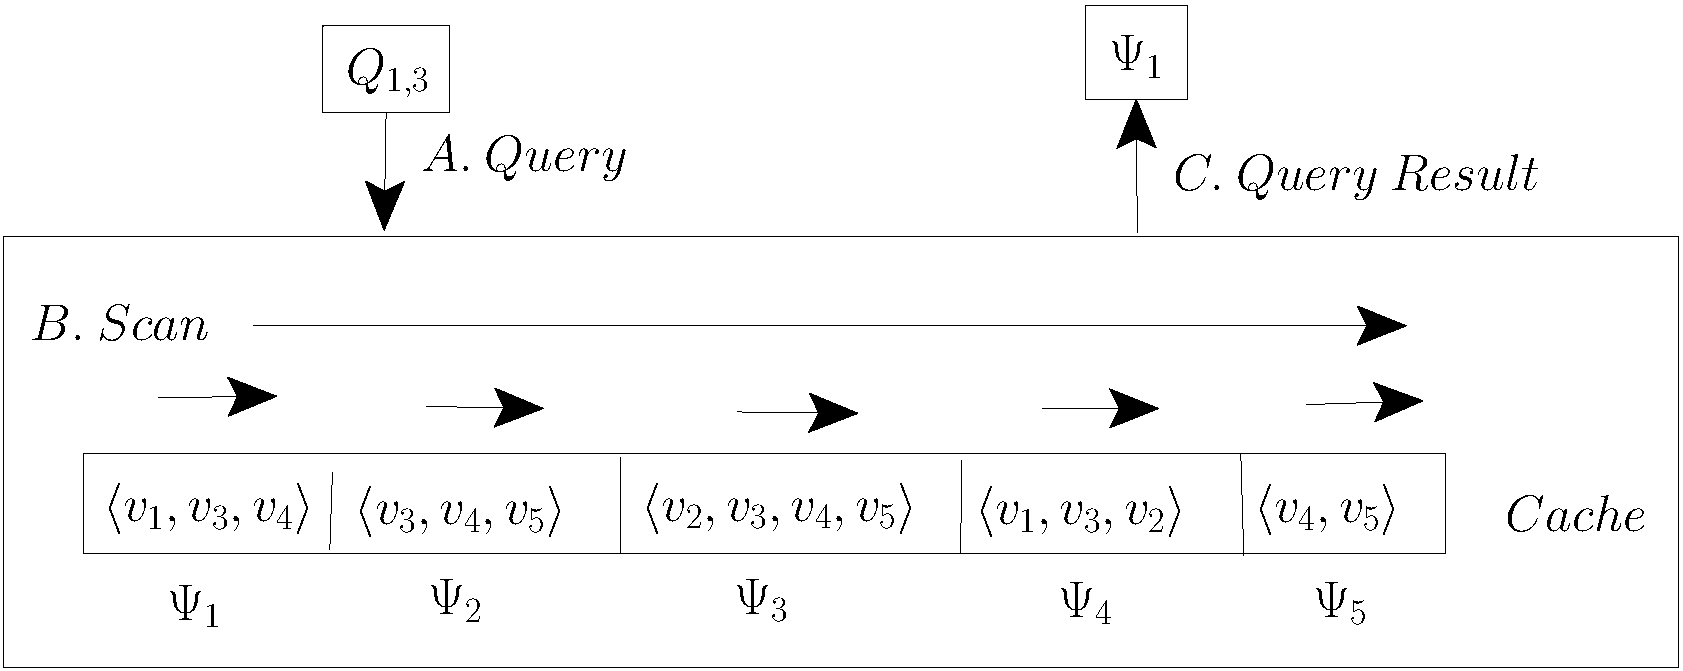
\includegraphics[width=0.45\textwidth]{figures/cachearray.pdf}
%        \caption{Simple array of paths.}
%  \label{fig:cachearray}
%\end{figure}


%\subsection{Simple array of paths inverted list}
%A simple, yet very effective, way to improve the search time of a cache represented by a simple array is to add an inverted list on top of the cache. We add an inverted list with node ids as keys and values being a list of array indices which holds paths containing specific node ids. By using such an inverted list we just need to do the intersection between the lists retrieved by querying the inverted list with the start and target node ids.





\begin{figure}[hbt]
  \center
  \begin{tabular}{cc}
    \begin{tabular}{c|l|}
        \cline{2-2}
        $\Psi_1$ & $v_1, v_3, v_4$ \\ \cline{2-2}
        $\Psi_2$ & $v_1, v_3, v_2$ \\ \cline{2-2}
        $\Psi_3$ & $v_2, v_3, v_4, v_5$ \\ \cline{2-2}
%        $\Psi_4$ & $v_3, v_4, v_5, v_6$ \\ \cline{2-2}
%        $\Psi_5$ & $v_3, v_4, v_5, v_7$ \\ \cline{2-2}
    \end{tabular}
    &
    \begin{tabular}{c|l|}
        \cline{2-2}
        $v_1$ & $\Psi_1, \Psi_2$ \\ \cline{2-2}
        $v_2$ & $\Psi_2, \Psi_3$ \\ \cline{2-2}
        $v_3$ & $\Psi_1, \Psi_2, \Psi_3$ \\ \cline{2-2}
        $v_4$ & $\Psi_1, \Psi_3$ \\ \cline{2-2}
        $v_5$ & $\Psi_3$ \\ \cline{2-2}
%        $v_6$ & $\Psi_4$ \\ \cline{2-2}
%        $v_7$ & $\Psi_5$ \\ \cline{2-2}
    \end{tabular}
    \\
    (a) path array & (b) inverted lists
  \end{tabular}
%        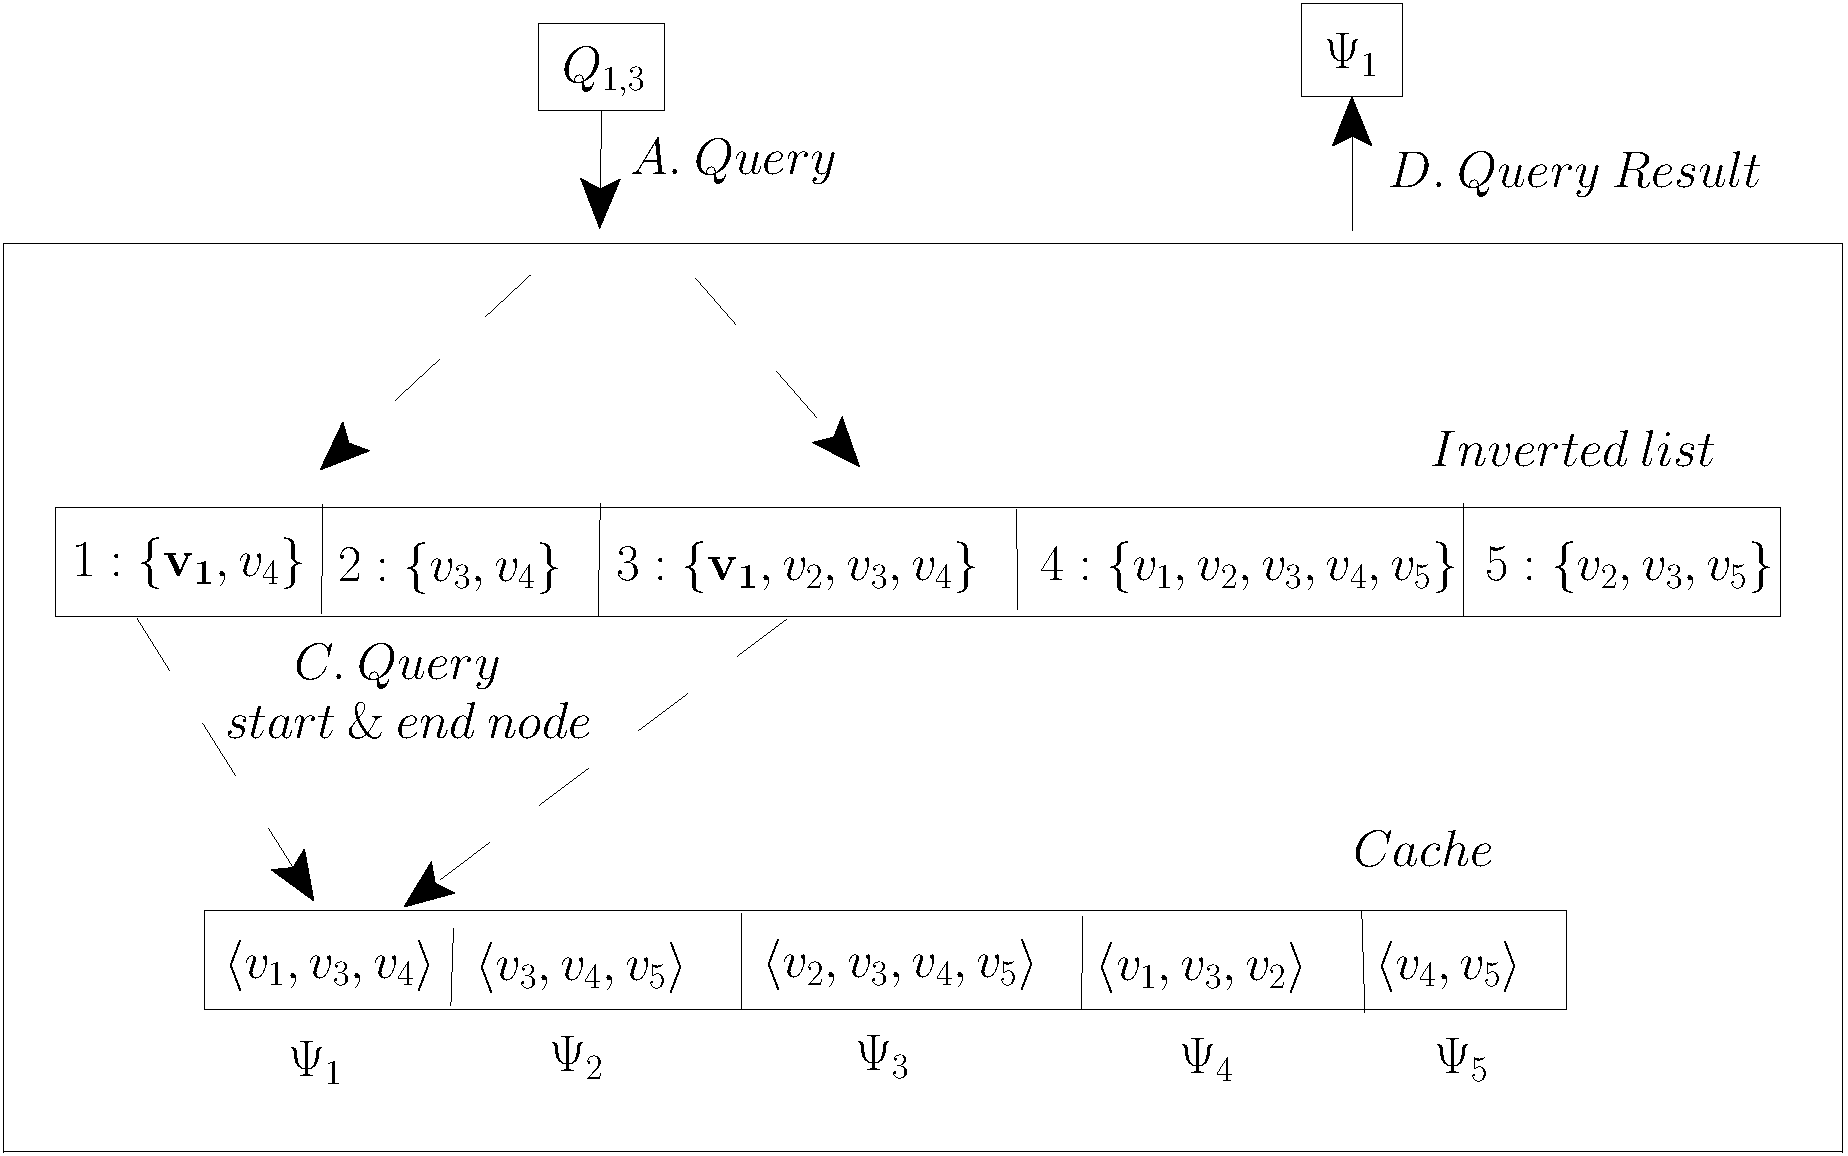
\includegraphics[width=0.50\textwidth]{figures/cachearrayinvertlist.pdf}
  \caption{Path array, with inverted lists}
  \label{fig:cacheinvertlist}
\end{figure}


%\stitle{Structure}
%


%\stitle{Query matching}
%



\stitle{Cache size analysis}
%
In previous sections, we only measure the cache size in terms of the paths/nodes in the cache,
but not the size of auxiliary structures (e.g., inverted lists).


Now, we measure the cache size accurately in an absolute unit (e.g., bits, bytes)
and consider both: (i) the sizes of paths/nodes in the path array, and
(ii) the sizes of inverted lists.
%In a real system, the cache budget $\mathcal{B}$ is given in terms of . Thus, we need to measure the total
%in terms of the total size of the data structures we employed.


Let $|\Psi|$ be the number of nodes in the path array, and $m$ be the number of paths in the path array.
Observe that an attribute with the domain size $x$ can be stored
as a binary string with $\mathcal{I}_x= \lceil \log_2 x \rceil$ bits.

In the path array, each node can be represented by $\mathcal{I}_{|V|}$ bits.
Thus, the path array occupies $|\Psi| \cdot \mathcal{I}_{|V|}$ bits.
%
In each inverted list, each path ID can be represented by $\mathcal{I}_m$ bits.
Note that the total number of path IDs in inverted lists equals to $|\Psi|$.
Thus, the inverted lists occupy $|\Psi| \cdot \mathcal{I}_m$ bits.
%
In summary, the total size of the structure is: $|\Psi| \cdot (\mathcal{I}_{|V|}+\mathcal{I}_m)$ bits.
%Observe that it is proportional to $|\Psi|$.



%In other words, it allows more paths to be fit.
% in turn, allows more paths to be fit


%The storage space of the cache structure


%The  in the problem refers .

%

%encode





%For an integer with the domain $[0,M)$, it takes $\lceil log_2 M \rceil$ bits to encode the integer.




%For the sake of readability, the measurement of cache size has been simplified in previous sections,
%which ignores the encoding length of a node, and the .

%We only view
%In previous sections, we simply count the cache size $|\Psi|$
%and express the cache budget $\mathcal{B}$ in terms of the number of nodes.
%These values do not capture the size of additional structures (e.g., inverted list).
%
%
%In the proxy/server, a memory buffer is allocated for the cache and other structures.
%The buffer size is expressed in terms of MBytes (e.g., 10 MBytes) rather than in terms of nodes.
%calculate the size of a cache based on
%the cache content in terms of the number of nodes.
%No additional memory beyond the buffer can be used.





\subsection{Compact Cache via Subgraph Model}\label{sec:cacheSubgraph}
% - solves goal 1, allows for more paths in cache, which should translate more cache hits.
%
We then propose a cache structure that consists of a subgraph $G_{\Psi}$ (see
Figure~\ref{fig:cachegraph}a) and inverted lists (see Figure~\ref{fig:cachegraph}b).
%
The same inverted lists from Figure~\ref{fig:cacheinvertlist}b are used in Figure~\ref{fig:cachegraph}b.
%When compared to the cache structure in Section~\ref{sec:cacheLookup},
The main difference is that the path array in Figure~\ref{fig:cacheinvertlist}a is now replaced by
a subgraph structure $G_{\Psi}$ that stores the adjacency lists of nodes that appear in the cache.
The advantage of this subgraph structure is that each node (and its adjacency list) is stored at most once in $G_{\Psi}$.

%We maintain a list of path ids with each node, with an entry for each cache item containing the node.


To check whether a query $Q_{s,t}$ can be answered by the cache, we just examine the inverted lists of $v_s$ and $v_t$
and follow the same procedure discussed in Section~\ref{sec:cacheLookup}.
There is a hit when the intersection of these two lists contains a path ID (say, $\Psi_j$).
To find the result path $P_{s,t}$, we start from source $s$ and visit a neighbor node $v$ whenever the inverted list of $v$ contains
$\Psi_j$.
%Finding the actual answer does however take a little more work, as we need to traverse the graph along the \spath query answer to know which nodes are in the list.
%This searches $\sum_{v_0}^{v_{|\spaths |}} v_i*|e_i|$ nodes, where $v_i \in V$ is a node on the \spath answer and $|e_i| \in E $ is the edge degree of $v_i$.


Figure~\ref{fig:cachegraph}c is a visualization of the structures in Figures~\ref{fig:cachegraph}a,b.
Note that the subgraph $G_{\Psi}$ only contains the adjacency lists of nodes that appear in the cache.
Let's take query $Q_{2,4}$ as an example.
First, we check the inverted lists of $v_2$ and $v_4$ of inverted lists in Figure~\ref{fig:cachegraph}b.
Their intersection contains a path ID ($\Psi_3$).
We then start from the source $v_2$ and visit its neighbor $v_3$ whose inverted list contains $\Psi_3$.
Next, we examine the unvisited neighbors of $v_3$, i.e., $v_1$ and $v_4$.
We ignore $v_1$ as its inverted list does not contain $\Psi_3$.
Finally, we visit $v_4$ and reach the target.
During the traversal, we obtain the shortest path: $\langle v_2, v_3, v_4 \rangle$.


%if the \spath id set intersection of $v_1$ and $v_5$ is non-empty Fig. \ref{fig:cachegraph}. Since there is a \spath (path 1) in the cache which can answer $Q_{1,5}$, we will do a search for all nodes between $v_1$ and $v_5$ which also includes path 1 in their \spath id set Fig. \ref{fig:cachegraph}. The edges taken when doing this search is shown with bold arrows. $v_2$ is also examined since it is connected to the actual path, but is ignored afterwards as $v_2$ does not have \spath id 1 in its set. Note that since both $v_1$ and $v_5$ has id 1 in their \spath id set, then there will always be a path between them. Once we have traversed the graph and found the answer to $Q_{1,5}$ we return the result Fig. \ref{fig:cachegraph}.


%maximizes the
%As such the goal of this representation is to reduce the overall execution time used on \spath calculation by increasing the number of paths in the cache so fewer queries may need to be calculated.
%The graph representation overall fulfills goal XXX by allowing more paths in the cache.

%The cache query time is slightly worse than when using an array with an inverted list.
%but it does unfortunately also impose some overhead to the query answer time, as each answer needs to be found in the graph (Fig. \ref{fig:cachegraph}C) once it has been confirmed (Fig. \ref{fig:cachegraph}B).



\begin{figure}[hbt]
  \center
  \begin{tabular}{@{}c@{ }c@{ }c@{}}
    \begin{tabular}{c|l|}
        \cline{2-2}
        $v_1$ & $v_3$ \\ \cline{2-2}
        $v_2$ & $v_3$ \\ \cline{2-2}
        $v_3$ & $v_1, v_2, v_4$ \\ \cline{2-2}
        $v_4$ & $v_3, v_5$ \\ \cline{2-2}
        $v_5$ & $v_4$ \\ \cline{2-2}
    \end{tabular}
    &
    \begin{tabular}{c|l|}
        \cline{2-2}
        $v_1$ & $\Psi_1, \Psi_2$ \\ \cline{2-2}
        $v_2$ & $\Psi_2, \Psi_3$ \\ \cline{2-2}
        $v_3$ & $\Psi_1, \Psi_2, \Psi_3$ \\ \cline{2-2}
        $v_4$ & $\Psi_1, \Psi_3$ \\ \cline{2-2}
        $v_5$ & $\Psi_3$ \\ \cline{2-2}
    \end{tabular}
    &
    \begin{tabular}{@{}c@{}}
    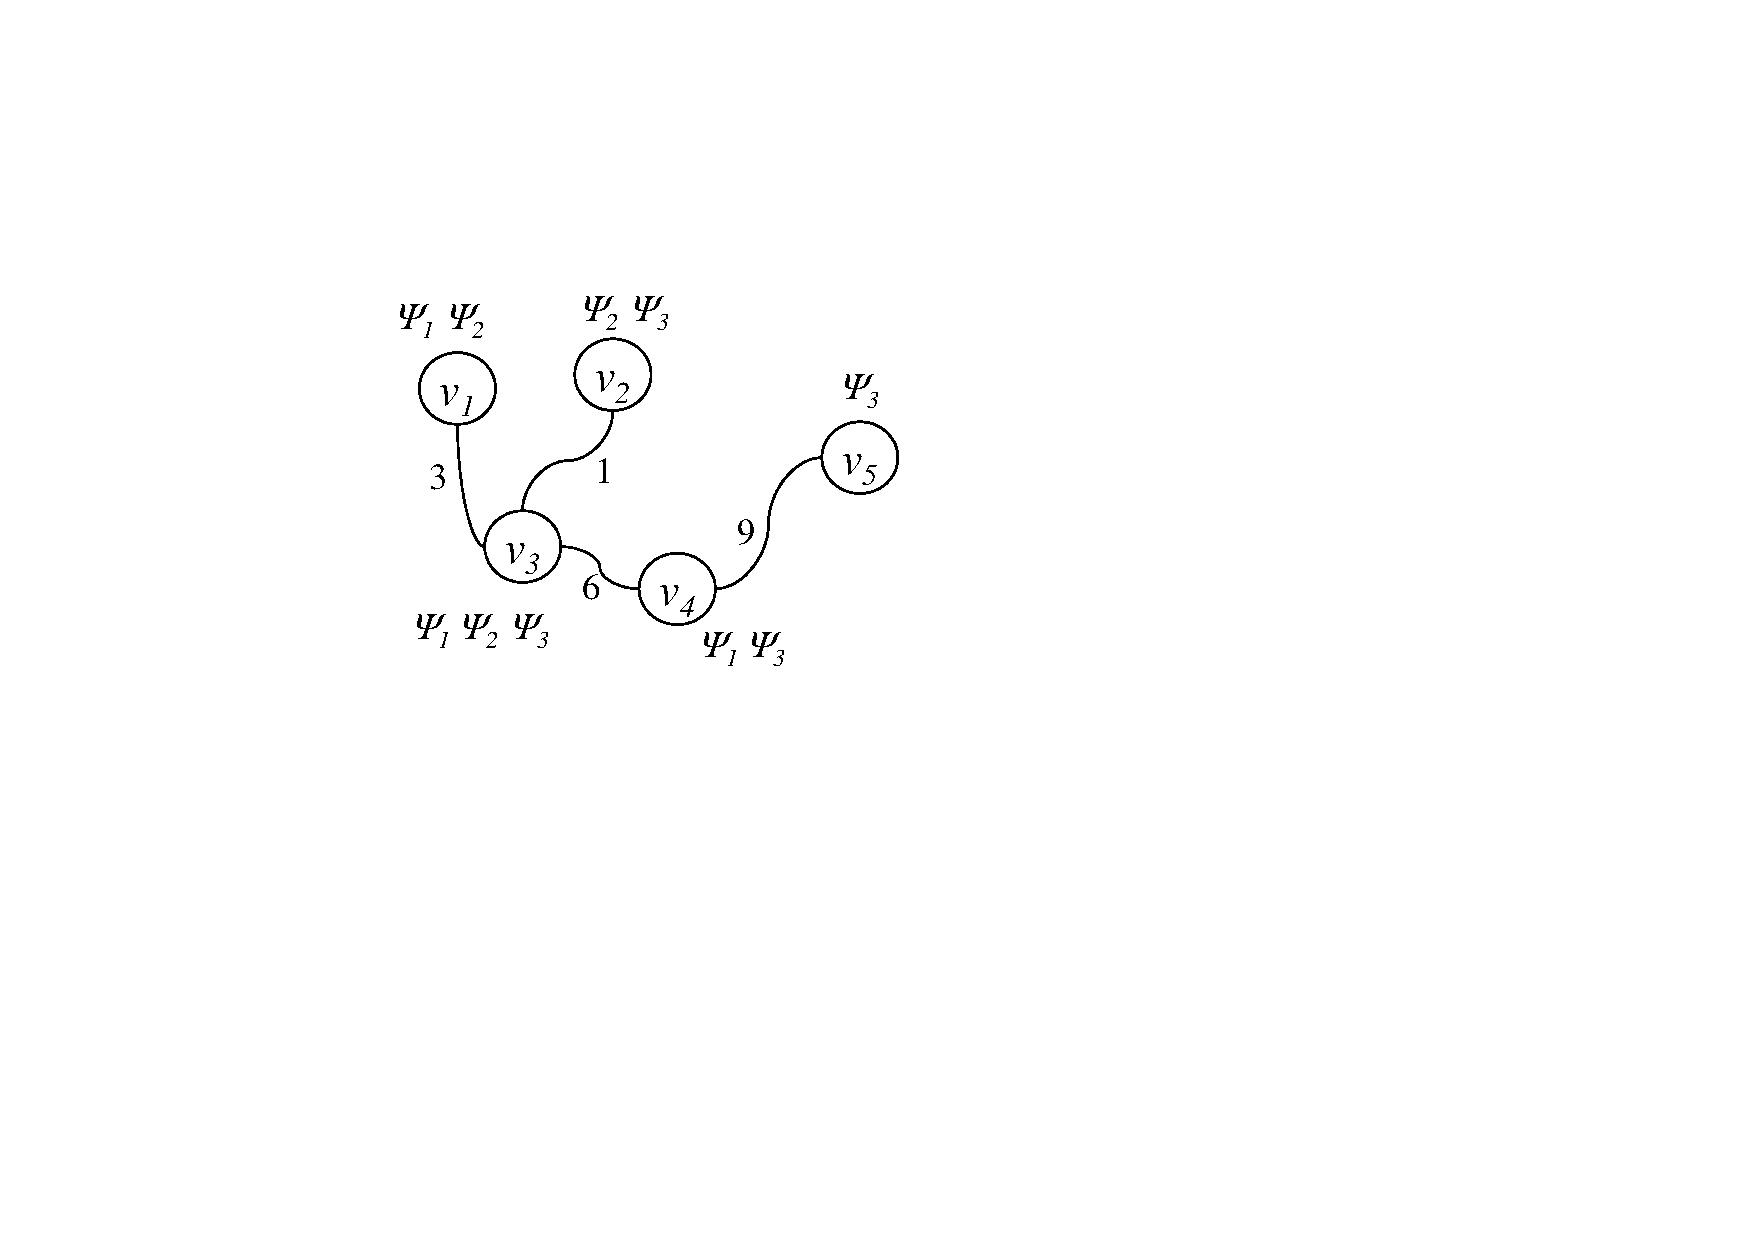
\includegraphics[width=0.45\columnwidth]{figures/cachegraph}
    \end{tabular}
    \\
    (a) subgraph $G_{\Psi}$ & (b) inverted lists & (c) visualization
  \end{tabular}
%        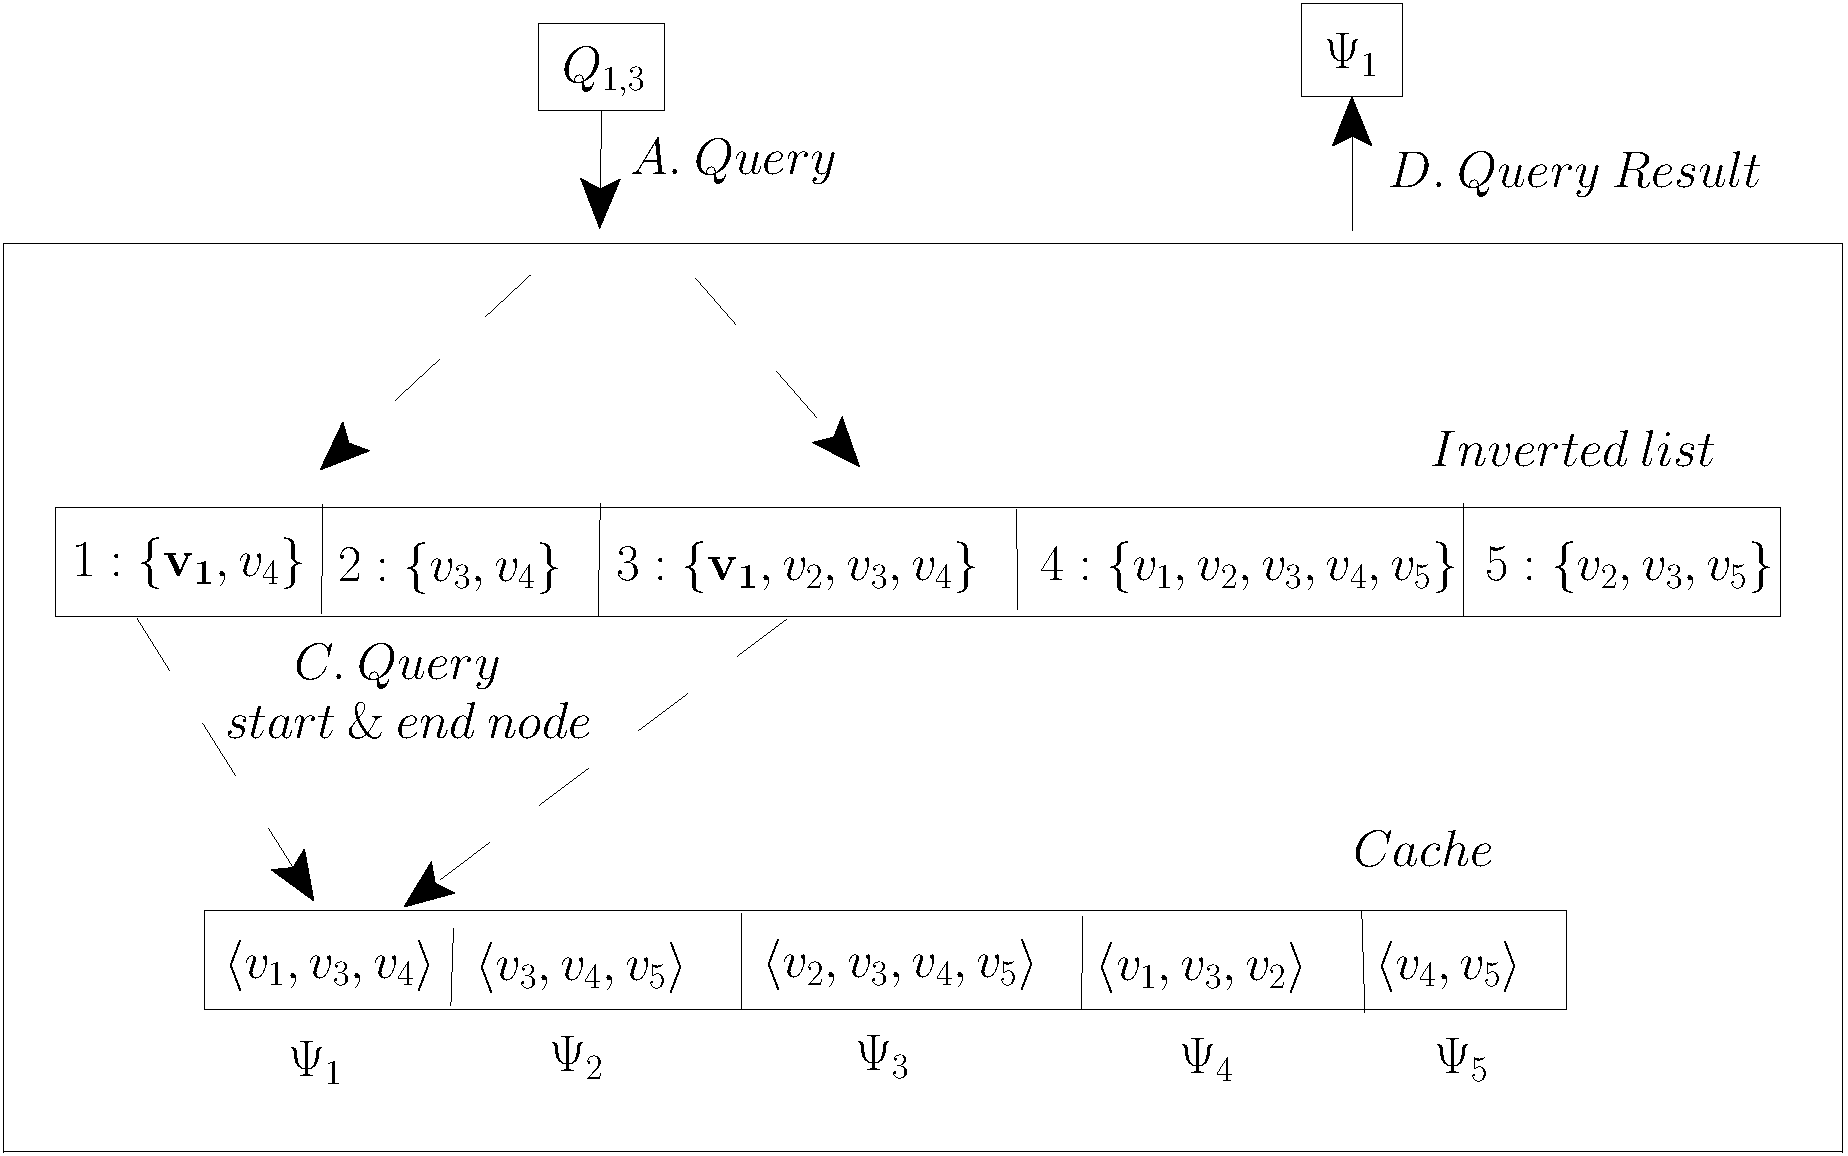
\includegraphics[width=0.50\textwidth]{figures/cachearrayinvertlist.pdf}
  \caption{Subgraph representation, with inverted lists}
  \label{fig:cachegraph}
\end{figure}




\stitle{Cache size analysis}
%
% maybe put this in a comparison in a later section
We proceed to analyze the cache size of the above cache structure.
As in Section~\ref{sec:cacheLookup}, we let $|\Psi|$ be the number of nodes in the cache, and $m$ be the number of paths in the cache.
%
Let $V_{\Psi} \subset V$ be the number of distinct nodes in the cache, and
$e$ be the average number of neighbors per node.


The inverted lists take $|\Psi| \cdot \mathcal{I}_m$ bits, as computed in the last section.
The subgraph occupies $|V_{\Psi}| \cdot e \cdot \mathcal{I}_{|V|}$ bits.
Thus, the total size of the structure is: $|V_{\Psi}| \cdot e \cdot \mathcal{I}_{|V|} + |\Psi| \cdot \mathcal{I}_m$ bits.

Note that $|V_{\Psi}|$ is upper bounded by $|V|$ and it is independent of the number of paths $m$ in the cache.
Thus, the subgraph representation is compact than the structure in Section~\ref{sec:cacheLookup}.
The saved space can then be used for accommodating additional paths into the cache,
in turn improving the benefit of the cache.



% \begin{itemize}
% \item Explain graph representation.
%     \begin{itemize}
%     \item how are paths represented
%     \item how is the search performance of the cache compared to previous array approach
%     \item solves goal 1, allows for more paths in cache, which should translate more cache hits.
%     \end{itemize}
% \item Explain subpath sharing.
%     \begin{itemize}
%     \item solves goal 1, allows for more paths in cache, translating to more cache hits. Unfortunately has a negative impact on goal 2 as it introduces some overhead in query time.
%     \item very compact representation
%     \end{itemize}
% \item most of the explanation should be tied to figure \ref{fig:cachegraph}
% \end{itemize}



\subsection{Compact Inverted Lists}\label{sec:cacheCompress}
%
%From our empirical findings, we observe that the inverted
In this section, we present two compression techniques for reducing the space consumption
of inverted lists. Again, the saved space can be used to accommodate more paths into the cache,
improving the benefit of the cache.



\stitle{Interval path ID compression}
%
This technique represents a consecutive sequence of path IDs $\Psi_i, \Psi_{i+1}, \Psi_{i+2}, \cdot, \Psi_j$ as an interval of path IDs $\Psi_{i,j}$.
In other words, these $j-i+1$ path IDs can be compressed into 2 path IDs.
The technique can achieve significant compression power when there are long consecutive sequences of path IDs in inverted lists.
% provide some motivation, elaborate here


Figure~\ref{fig:compressedlist}a shows the original inverted lists
and Figure~\ref{fig:compressedlist}b shows the compressed inverted lists obtained by this compression.
For example, the inverted list of $v_3$ ($\Psi_1, \Psi_2, \Psi_3$) is compressed into the interval $\Psi_{1,3}$.




%An optimization to the graph representation is to not directly represent each path id in the path id set of each node. We can do this by collapsing each %continues sequence of path ids. Table \ref{tab:compressedlist} shows how the id sets for each node in figure \ref{fig:cachegraph} can be collapsed and what %the savings are in terms of how many more path ids we have space for.



\stitle{Prefix path ID compression}
%
This technique first identifies inverted lists that share the same prefix,
and then expresses an inverted list by using the other inverted list as prefix.

% a consecutive sequence of path IDs $\Psi_i, \Psi_{i+1}, \Psi_{i+2}, \cdot, \Psi_j$ as an interval of path IDs $\Psi_{i,j}$.
Let's consider the original inverted lists in Figure~\ref{fig:compressedlist}a.
The inverted list of $v_1$ is the prefix of the inverted list of $v_3$.
Figure~\ref{fig:compressedlist}c shows the compressed inverted lists produced by this compression.
%
In the compressed inverted list of $v_3$, it suffices to store path IDs (e.g., $\Psi_3$)
that do not appear in its prefix. The remaining path IDs of $v_3$ can be retrieved by following the parent ($v_1$)
of its inverted list.

Both compression techniques can be combined together in order to achieve a
higher compression power.


%\begin{table}
%\center
%\begin{tabular}{|l|l|l|}\hline
%Node 	& Compressed list & Num. path ids saved \\\hline
%$v_1$ 	& $\langle 1, 3 \rangle$ 	& 0 \\\hline
%$v_2$ 	& $\langle2, 5 \rangle$ 	& 0 \\\hline
%$v_3$ 	& $\langle 1-3, 5-6 \rangle$ 	& 1 \\\hline
%$v_4$ 	& $\langle 1-6 \rangle$ 	& 4 \\\hline
%$v_5$ 	& $\langle 1-2, 4-6 \rangle$ 	& 1 \\\hline
%$v_6$ 	& $\langle 1-2, 6 \rangle$ 	& 0 \\\hline
%$v_7$ 	& $\langle 4 \rangle$ 		& 0 \\\hline
%
%\end{tabular}
%\caption{Compressed list content and the space saved by using them.}
%\label{tab:compressedlist}
%\end{table}



\begin{figure}[hbt]
  \center
  \begin{tabular}{@{}c@{ }c@{ }c@{}}
    \begin{tabular}{c|l|}
        \cline{2-2}
        $v_1$ & $\Psi_1, \Psi_2$ \\ \cline{2-2}
        $v_2$ & $\Psi_2, \Psi_3$ \\ \cline{2-2}
        $v_3$ & $\Psi_1, \Psi_2, \Psi_3$ \\ \cline{2-2}
        $v_4$ & $\Psi_1, \Psi_3$ \\ \cline{2-2}
        $v_5$ & $\Psi_3$ \\ \cline{2-2}
    \end{tabular}
    &
    \begin{tabular}{c|l|}
        \cline{2-2}
        $v_1$ & $\Psi_{1-2}$ \\ \cline{2-2}
        $v_2$ & $\Psi_{2-3}$ \\ \cline{2-2}
        $v_3$ & $\Psi_{1-3}$ \\ \cline{2-2}
        $v_4$ & $\Psi_1, \Psi_3$ \\ \cline{2-2}
        $v_5$ & $\Psi_3$ \\ \cline{2-2}
    \end{tabular}
    &
    \begin{tabular}{c|l|c|}
        \multicolumn{3}{c}{~~~~~~~~content~~~~parent} \\
        \cline{2-3}
        $v_1$ & $\Psi_1, \Psi_2$ & NIL \\ \cline{2-3}
        $v_2$ & $\cdots$ & $\cdots$ \\ \cline{2-3}
        $v_3$ & $\Psi_3$ & $v_1$ \\ \cline{2-3}
        $v_4$ & $\cdots$ & $\cdots$ \\ \cline{2-3}
        $v_5$ & $\cdots$ & $\cdots$ \\ \cline{2-3}
    \end{tabular}
    \\
    (a) original & (b) interval & (c) prefix \\
                 &  compressed & compressed \\
  \end{tabular}
  \caption{Compressed inverted lists}
  \label{fig:compressedlist}
\end{figure}



% \subsection{helping text}
% \begin{enumerate}
% \item Introduce the problem setting in more detail than in the introduction and formally define the problem and what exactly we aim to solve in this paper.\\
% \item show where exactly the proposed cache is located in an online \spath service providers system.
% \item State goal 1(a) and 2(b)
% 	\begin{enumerate}
% 	\item Reduce the time spent executing the \spath algorithm. - The \spath algorithm is usually the single most CPU expensive task at a \spath service provider.
% 	\item Reduce the time spent on overhead. - Introducing a cache will also add some overhead, this overhead not desirable and should  be minimized.
% 	\end{enumerate}
% \item Introduce the overall setting which our solution work in and give a table of notation for reader reference.
% \end{enumerate}



%% 




%NumLandmarks=20
%
%NumBuckets=10
%
%NumSamples=100


% draw tables HERE ...







\section{Experiments}\label{sec:experiments}
%
In this section, we evaluate the performance of our methods with our competitors on real datsets.
% We will conduct experiments
We have implemented two variants of our methods (SPC and SPC*).
%for extracting statistics of queries, benchmarking the cost of a shortest path call,
%and selecting promising paths from a query log $\mathcal{QL}$ into the cache.
They share the same techniques in Section~\ref{sec:BenefitDriven},
and only differ in their cache structures:
(i) SPC uses a path array cache (Section~\ref{sec:cacheLookup}), and (ii) SPC* uses the compressed graph cache (Sections~\ref{sec:cacheSubgraph},\ref{sec:cacheCompress}).
%
Our competitors are LRU (a dynamic caching method) and HQF (a static caching method).
They have been introduced in Section~\ref{sec:competitors}.
All the above methods are written in C++.
We conduct our experiments on an Intel i7 3.4GHz PC running Debian.

%  (ii) SPC$^+$ uses a graph cache (Section~\ref{sec:cacheSubgraph}),
%SPC, our method, with the 3 cache representation schemes - List cache, Graph cache, Compressed Graph cache - described in section

We will evaluate the above methods for a cache located at the proxy, and for a cache located at the server.
For the proxy scenario, the performance measure is the hit ratio.
For the server scenario, the performance measures are: (i) the total running time of the server,
and (ii) the total number of road network nodes visited.


%in both the proxy
%well both when considering the Proxy and Server scenario

%To compare how well we have done, we have implemented two baseline competitors, LRU and HQF. LRU is a dynamic caching method which evicts the Least recently used cache item if there is no space in the cache for new entries. HQF adds to the cache, the \spaths from the most frequent start-/end-points in the training data.





%Aalborg: total nodes in SPs from training set: 352032 in 1643 paths

%Beijing: total nodes in SPs from training set: 316400 in 6479 paths



%This is the most common usage of static caching in the web caching literature \cite{BaezaYates07}.


% In this section, we present the results of performance
% experiments, demonstrating the efficiency and realworld applicability of the proposed algorithms. We


\subsection{Experimental Setting}
%
We are unable to obtain real query log from online shortest path services (e.g., Google Map), due to their privacy policies.
Thus, we can only simulate a query log from a trajectory dataset.
For each trajectory, we extract its start location and its end location as the
source $v_s$ and destination $v_t$ of a shortest path query respectively.

We have used two real datasets and their details can be found in Table~\ref{tab:datasetsize}.
Each dataset consists of (i) a collection of trajectories (which can be used to simulate a query log), and 
(ii) a corresponding road network for the trajectories.

%Which historical query datasets do we have, and what is their size and origin.

%- Aalborg: Query workload from and around the Danish city of Aalborg

%- Beijing: Query workload from Beijing



Following the experimental methodology of static caching~\cite{Ozcan2011},
we divide the query log into two equal sets.
The {\em historical query log} set is used for defining query frequencies and
for filling the cache content.
The {\em query workload set} set can only used for testing the performance of our method.


%We do not give a default size for the query-datasets Maps, as we will execute all of our tests, described in section \ref{subsec:expProxy} and \ref{subsec:expServer}, for each dataset.


\begin{table}
\center
\begin{tabular}{|c|r|r|r|}\hline
Dataset & $\#$ Trajectories / Queries & $\#$ Nodes & $\#$ Edges \\\hline
Aalborg & 4.401  & 129.680 & 137.470 \\\hline
Beijing & 12.928 & 76.226 & 85.882 \\\hline
\end{tabular}
\caption{Description of real datasets}
\label{tab:datasetsize}
\end{table}
%% Aalborg = Aalborg
%% Beijing = Beijing


%GPS trajectories

%according to XXX l

%The size of training and test query datasets are given already. The size of each dataset, as well as the map they are captured on, is given in table \ref{tab:datasetsize}.



%% Aalborg = Aalborg
%% Beijing = Beijing


%We do not give a default size for the query-datasets Maps, as we will execute all of our tests, described in section \ref{subsec:expProxy} and \ref{subsec:expServer}, for each dataset.




All caching methods, SPC, SPC*, HQF, and LRU, share a number of common settings which, unless stated otherwise, will be set to their default values:
The number of levels in the kD-tree is 14 (i.e. 16,384 regions). We will use the list cache representation as the default cache representation, where each vertex use one byte. The default cache size is set to 625 kB.


The default cache size, as well as the maximum cache size in later experiments (Fig.~\ref{fig:cSizeVsHitRatio}, \ref{fig:cacheSizeVsHitRuntime}, \ref{fig:cacheSizeVsNodesvisited}), is choosen baring in mind the size of the Aalborg and Beijing query logs. 
Had we had access to large datasets of real query logs, from online shortest path serveice providers, we would use a large cache size like 1 GB.

% 
% 
% The size of our datasets is the limiting factor
% 



\label{fig:cacheSizeVsHitRuntime}

\label{fig:cacheSizeVsNodesvisited}


% - Which parameters are common for all tests
% - What are the ranges/values each parameter can take.
% - Which parameters are set to a default value unless otherwise stated (and what are the default values)
% - Which methods, and in which configuration, do we consider.



\subsection{Caching in the Proxy Scenario}\label{subsec:expProxy}
%
In the proxy scenario, the shortest path call API would issue a shortest path query to the server,
rather than performing computation by itself (see Section~\ref{sec:benchmark}).
Since the total cost is dominated by the communication round-trip time with server,
we use the cache hit ratio as the performance measure in this scenario.

For both datasets we vary the cache size and kD-tree levels to show the impact on the cache hit ratio. We have implemented a number of optimizations to the cache storage (See sec. \ref{sec:CacheStruct}) and show their impact on the cache hit ratio.


\stitle{Effect of the cache size}
%
In Figure~\ref{fig:cSizeVsHitRatio}, we measure the hit ratio of the methods
while varying the cache size from 1 kB to 5 MB.


\begin{figure}[htb]
\center
  \begin{tabular}{@{}c@{ }c@{}}
     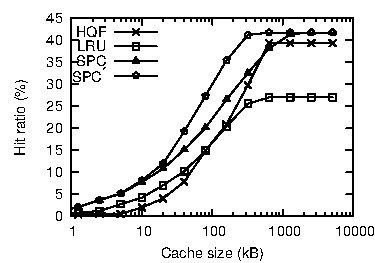
\includegraphics[width=0.5\columnwidth]{figures/cachesize_hitratio_aal.pdf}
     &
     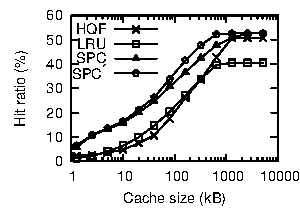
\includegraphics[width=0.5\columnwidth]{figures/cachesize_hitratio_bei.pdf}
      \\
     (a) Aalborg & (b)  Beijing
     \end{tabular}
\caption{Hit ratio vs. cache size }
\label{fig:cSizeVsHitRatio}
\end{figure}

% \begin{itemize}
% \item We can see SPC* performs much better than competitors
% \item LRU perform well on small cache sizes, but the cache hit ratio quickly level out and stop growing, thus LRU is not scalable.
% \item HQF performance is very consistent, with the hit ratio varying only slightly. The hit ratio does however stay at just over 1\% for Aalborg experiments and around 0.2\% for Beijing experiments. It is not usable
% \item We observe that SPC initially does not grow as fast as LRU, but the growth continues as we increase cache size, unlike for LRU.
% \item SPC* grows faster than LRU and gets better cache hit ratio at all cache sizes than LRU and SPC, except for the smallest cache size.
% \item The test on the Aalborg vs. Beijing sets show that SPC performs much better on the Aalborg set, where as LRU performs about 50\% worse. This can be explained by the fact that both methods rely on users behaving consistently over time, but where SPC relies on global consistency in user behavior, LRU need local consistency too. This makes SPC/SPC* more robust and we can expect them to always outperform LRU.
% \end{itemize}
{\color{red}
We can see that LRU consistently perform worse than SPC and SPC$^*$ for all cache sizes. The cache hit ratio stabilizes at about 26 and 40\% for Aalborg and Beijing respectively. Since LRU levels out at a much lower cache hit ratio than all of it's competitors it is not a suitable choice for \spath cacheing.


The performance of HQF is quite low at smaller cache sizes, 

The performance of HQF is very consistent, with the hit ratio varying only slightly. The hit ratio stays at just over 1\% for Aalborg experiments and around 0.2\% for Beijing experiments. The low hit ratio makes it not scalable and unusable for \spath caching.
}

SPC does not grow as fast as LRU for smaller cache sizes, but while the growth of LRU quickly stabilizes then SPC continues to grow and outperforms both LRU and HQF.
SPC* outperforms both LRU and SPC by a large margin, only shortly having a lower cache hit ratio at smaller cache sizes. The test on Aalborg vs. Beijing  show that SPC performs much better on the Aalborg set, where as LRU performs about 50\% worse. This can be explained by the fact that both methods rely on users behaving consistently over time, but where SPC relies on global consistency in user behavior, LRU need local consistency too. This makes SPC/SPC* more robust and we expect them to always outperform LRU.



\stitle{Effect of the kD-tree level}
%
In Figure~\ref{fig:levelVsHitRatio}, we vary the kD-tree level from 8 to 18 levels and show that using a kD-tree of about 14 levels can significantly increase the cache hit ratio of both the Aalborg and Beijing dataset. SPC* performs better than SPC.


\begin{figure}[htb]
\center
  \begin{tabular}{@{}c@{ }c@{}}
     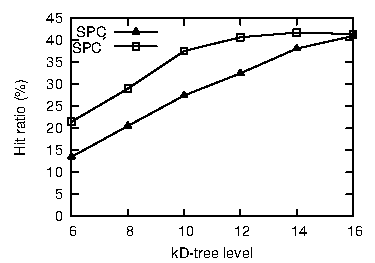
\includegraphics[width=0.5\columnwidth]{figures/split_hitratio_aal.pdf}
     &
     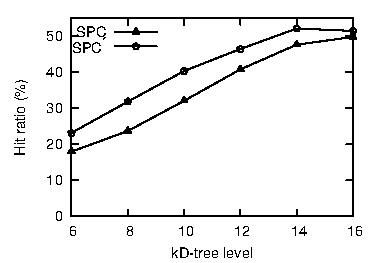
\includegraphics[width=0.5\columnwidth]{figures/split_hitratio_bei.pdf}
      \\
     (a) Aalborg & (b)  Beijing
     \end{tabular}
\caption{Hit ratio vs. Levels}
\label{fig:levelVsHitRatio}
\end{figure}

On both dataset SPC* outperforms SPC by a large margin. On the city X dataset SPC* achieves more than a 50\% increase in hit ratio, and when compared to SPC, it achieves a relative performance gain of 500-900\% at low levels up to the peak performance at level 14.
On the Y dataset SPC* gets a lower hit ratio, but it still achieves more than 50\% cache hit ratio. The results are still very impressive, with SPC* performing 200-400\% better than SPC at all levels.

% \noindent
% \begin{tabular}{|l |p{0.58\columnwidth} |l |}
% \hline
% \textbf{Parameter} & \textbf{Meaning / used for} & \textbf{Standard value} \\\hline
% Mapfile & The map which the test is performed on & \\\hline
% NumQueries & Number of \spath queries in test & \\\hline
% QuerySet & which dataset is used to provide queries & \\\hline
% TrainSet & For generating region statistics, which dataset is used & \\\hline
% CacheSize & Size of cache in bits & \\\hline
% cacheType & Type of cache representation (list/graph) & \\\hline
% kD-tree & Hight of the kD-tree & \\\hline
% avgLenght & Average length of a shortest path & \\\hline
% \end{tabular}

% Write experiments to examine performance of goal 1 \& 2
% Test ideas (several ideas may be combined, like item 1 can be done on all datasets from item 2):\\
% \begin{itemize}
% \item increase kd-tree hight from 0-18
% \item different maps [Oldenburg, Aalborg, Beijing]
% \item compare cache type performance
% \item compare with baseline methods. [LRU dynamic, Dynamic(maxLevel)]
% \item vary the cache size [10.000-2560000]
% \item vary number of queries. [only for synthetic data]
% \end{itemize}

\subsection{Caching in the Server Scenario}\label{subsec:expServer}
%
In the server scenario, the shortest path API has to invoke a shortest path algorithm.
Thus, the running time is the most important performance measure. We also measure the number of nodes visited in a shortest path algorithm, which serves an indicator of the running time.
%On a server our aim is slightly different than on the Proxy, as we also have to consider that there may be some paths that are so small that it may be cheaper to simply re-calculate the result, instead of caching it.
%For the server scenario we will test the cache hit ratio, running time, and Nodes visited.
%For all three experiments
%We will vary kD-tree levels and cache size in the following experiments.
As a case study, we use the Dijkstra's algorithm as the shortest path algorithm.

In the following experiments, the running time (and nodes visited) refer to the total running time (and nodes visited) for processing the entire query workload. The running time is measured in the unit of seconds.





\stitle{Estimation of shortest path running cost}
%
First, we test the estimation error of our cost estimation technique proposed in Section~\ref{sec:benchmark}.
We measure the error percentage in terms of the relative error between the actual cost and the estimated cost.
Table~\ref{tbl:estcost} shows the estimation error of our technique
as a function of: (a) the number of landmark $|U|$, and (b) the size of the samples $S$.
The default values are: $|U|=20$ and $S=100$.
The majority of errors are below 30\% and thus our estimation technique is reasonably accurate.


%% Aalborg: average cost = 136347/2 = 68173
%%  Beijing: average cost = 79603/2 = 39801
%  average because random node chosen



\begin{table}
\center
\begin{tabular}{cc}
    \begin{tabular}{|c|c|c|}
    \hline
    $|U|$ & Aalborg & Beijing \\ \hline \hline
     5 & 35.5 & 33.3 \\ \hline
     10 & 25.4 & 28.2 \\ \hline
     20 & 22.2 & 23.9 \\ \hline
     40 & 19.4 & 23.0  \\ \hline
     80 & 19.9 & 21.9 \\ \hline
    \end{tabular}
    &
    \begin{tabular}{|c|c|c|}
    \hline
    $S$ & Aalborg & Beijing \\ \hline \hline
     25 & 23.4 & 28.8 \\ \hline
     50 & 20.7 & 28.4 \\ \hline
     100 & 22.2 & 23.9 \\ \hline
     200 & 20.4 & 22.7 \\ \hline
     400 & 21.1 & 21.3 \\ \hline
    \end{tabular}
    \\
    (a) varying number of landmark $|U|$ & (b) varying sample size $S$
\end{tabular}
    \caption{Average error percentage of cost estimation}
    \label{tbl:estcost}
\end{table}








%
\stitle{Effect of the kD-tree level}
%
In Figure~\ref{fig:levelVsHitRatio}, we again vary the kD-tree level from 8 to 18 levels. All three experiments shows a consistent advantage of using SPC* over SPC. SPC* still has an even higher advantage than in the proxy scenario, performing around 950\% better than SPC at its best. SPC, however, has a very low hit ratio in the server scenario, on both the city X and Y datasets. In figure \ref{fig:levelVsruntime}a and b we can see that SPC* is very fast at answering the query workload. SPC has a quite stable time in both figure\ref{fig:levelVsruntime}a and b, while the time for SPC* to answer the query workload actually decreases with more regions. In figure \ref{fig:levelVsNodesvisited} we can see that SPC* visits far fewer nodes than SPC, during shortest path calculations. This is expected since SPC* can answer many more queries from its cache.




\begin{figure}[htb]
\center
  \begin{tabular}{@{}c@{ }c@{}}
     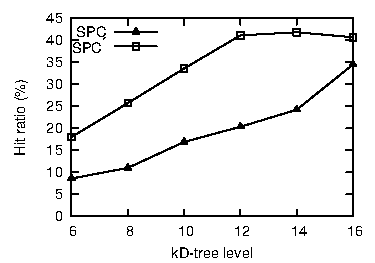
\includegraphics[width=0.5\columnwidth]{figures/split_hitratio_aal_server.pdf}
     &
     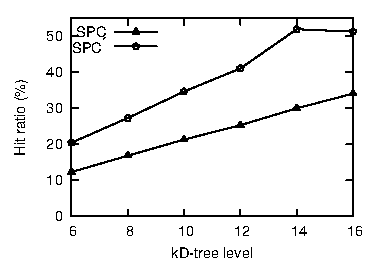
\includegraphics[width=0.5\columnwidth]{figures/split_hitratio_bei_server.pdf}
      \\
     (a) Aalborg & (b)  Beijing
     \end{tabular}
\caption{Hit ratio vs. Levels}
\label{fig:levelVsHitRatio}
\end{figure}

\begin{figure}[htb]
\center
  \begin{tabular}{@{}c@{ }c@{}}
     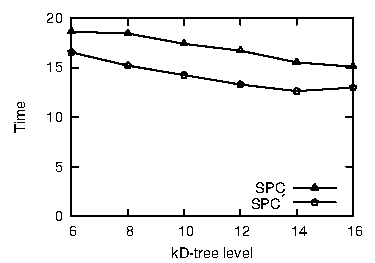
\includegraphics[width=0.5\columnwidth]{figures/split_runtime_aal_server.pdf}
     &
     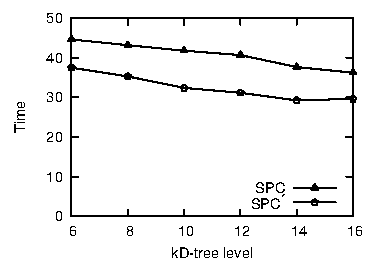
\includegraphics[width=0.5\columnwidth]{figures/split_runtime_bei_server.pdf}
      \\
     (a) Aalborg & (b)  Beijing
     \end{tabular}
\caption{Runtime vs. Levels}
\label{fig:levelVsruntime}
\end{figure}

\begin{figure}[htb]
\center
  \begin{tabular}{@{}c@{ }c@{}}
     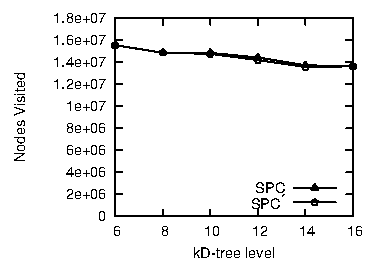
\includegraphics[width=0.5\columnwidth]{figures/split_nodes_aal_server.pdf}
     &
     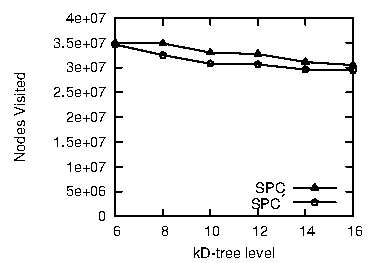
\includegraphics[width=0.5\columnwidth]{figures/split_nodes_bei_server.pdf}
      \\
     (a) Aalborg & (b)  Beijing
     \end{tabular}
\caption{Nodes Visited vs. Levels}
\label{fig:levelVsNodesvisited}
\end{figure}






\stitle{Effect of the cache size}
%
In the following experiments, we vary the cache size and observe the effect on the running time and nodes visited during shortest path calculations.






\begin{figure}[htb]
\center
  \begin{tabular}{@{}c@{ }c@{}}
     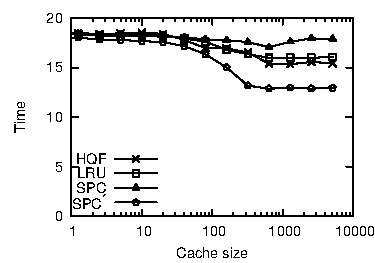
\includegraphics[width=0.5\columnwidth]{figures/cachesize_runtime_aal.pdf}
     &
     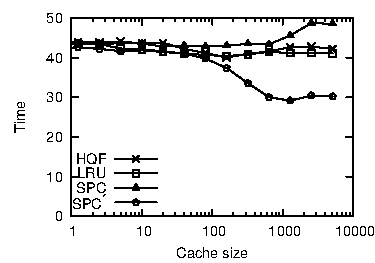
\includegraphics[width=0.5\columnwidth]{figures/cachesize_runtime_bei.pdf}
      \\
     (a) Aalborg & (b)  Beijing
     \end{tabular}
\caption{Runtime vs. Cache Size}
\label{fig:cacheSizeVsHitRuntime}
\end{figure}

In Figure \ref{fig:cacheSizeVsHitRuntime} and \ref{fig:cacheSizeVsNodesvisited}, for both the city X and Y dataset,  we can see that the graph looks similar to Figure \ref{fig:cSizeVsHitRatio}, but in the upside-down manner. This is to be expected, since a higher cache hit ratio gives fewer \spath calculations, and a lower runnig time when answering queries.

\begin{figure}[htb]
\center
  \begin{tabular}{@{}c@{ }c@{}}
     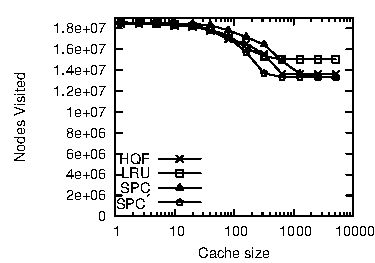
\includegraphics[width=0.5\columnwidth]{figures/cachesize_nodes_aal.pdf}
     &
     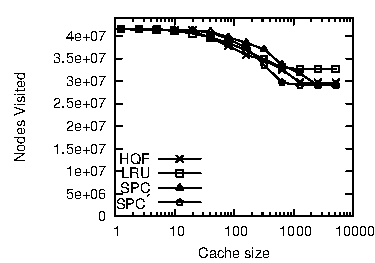
\includegraphics[width=0.5\columnwidth]{figures/cachesize_nodes_bei.pdf}
      \\
     (a) Aalborg & (b)  Beijing
     \end{tabular}
\caption{Nodes Visited vs. Cache Size}
\label{fig:cacheSizeVsNodesvisited}
\end{figure}




\section{Conclusion}\label{sec:conclusion}
%
In this paper, we have studied the caching of shortest paths in the proxy scenario and the server scenario.

We formulate a benefit model for capturing the benefit of a path in terms of its frequency and processing it.
We also propose an estimation method for estimating the cost of a specific shortest path query on any arbitrary
shortest path algorithm.
Our experimental results on real data show that our proposed cache selection algorithm is able to
achieve high hit ratio and reduce the running time.
Also, our proposed cache structures can further improve the lookup performance and maximize the utilization of cache space.


%select important paths in the cache in order to optimize the performance. Our


\section*{Acknowledgment}
%
We thank Eric Lo, Jianguo Wang, and the anonymous reviewers for their insightful comments.



\bibliographystyle{abbrv}
\bibliography{spcache}


\end{document}



%\usepackage{balance}
%\usepackage{url}
%\usepackage{times}
%%For math symbols like number classes
%\usepackage{amsfonts}
%\usepackage{amssymb}
%%\usepackage{amsthm}
%%\usepackage{floatflt}
%\usepackage{wrapfig}
%\usepackage{multirow}
%\usepackage{color}
%
%\usepackage[T1]{fontenc}
%\usepackage{hyperref}
%\usepackage{amsmath}
%\usepackage{acronym}
%\usepackage{xspace} % mellemrum efter forkortelser fra acronym package.
%\usepackage{longtable}
%\usepackage{graphicx}
%\usepackage{graphics}
%\usepackage{slashbox}
%\usepackage{pstricks}
%
%% \usepackage[cmex10]{amsmath}
%% \usepackage[pdftex]{graphicx}
%% \usepackage[pdftex]{graphics}
%
%
%% \usepackage[boxed,linesnumbered,vlined,slide]{algorithm2eCustom}
%\usepackage[boxed,linesnumbered,vlined,ruled]{algorithm2eCustom}
%
%\usepackage{cite}
%
%
%\newtheorem{thm}{Theorem}[section]
%\newtheorem{cor}[thm]{Corollary}
%\newtheorem{lemma}[thm]{Lemma}
%
%
%\newcommand{\ffh}[1]{\textbf{TODO: \textit{#1}}} 
\newcommand{\baseline}{Baseline \xspace} 
\newcommand{\dynamgrid}{Dynamic Grid \xspace}
\newcommand{\md}{\mdns \xspace}
\newcommand{\mdns}{MD}
\newcommand{\mds}{\mdsns \xspace}
\newcommand{\mdsns}{MDs}
\newcommand{\ls}{\lsns \xspace}
\newcommand{\lsns}{LS}
\newcommand{\lss}{\lssns \xspace}
\newcommand{\lssns}{LSs}
\newcommand{\ff}{\ffns \xspace}
\newcommand{\ffns}{\textsc{FriendLocator}}
\newcommand{\ffs}{\ffsns \xspace}
\newcommand{\ffsns}{\textsc{FriendLocators}}
\newcommand{\hc}{\hcns \xspace}
\newcommand{\hcns}{\texttt{Hide\&Crypt}}
\newcommand{\vl}{\vlns \xspace}
\newcommand{\vlns}{\textsc{VicinityLocator}}
\newcommand{\vls}{\vlsns \xspace}
\newcommand{\vlsns}{\textsc{VicinityLocators}}
\newcommand{\lmg}{\lmgns \xspace}
\newcommand{\lmgns}{LMG}
\newcommand{\lmgs}{\lmgsns \xspace}
\newcommand{\lmgsns}{LMGs}
\newcommand{\ttslong}{\ttslongns \xspace}
\newcommand{\ttslongns}{Trusted Third-party Server}
\newcommand{\tts}{\ttsns \xspace}
\newcommand{\ttsns}{TTS}
\newcommand{\iuns}{IU}
\newcommand{\rfns}{RF}
\newcommand{\iu}{\iuns \xspace}
\newcommand{\rf}{\rfns \xspace}
\newcommand{\iusns}{IUs}
\newcommand{\rfsns}{RFs}
\newcommand{\ius}{\iusns \xspace}
\newcommand{\rfs}{\rfsns \xspace}


\newcommand{\lpar}{(}
\newcommand{\rpar}{)}

\SetKwBlockLRS{LRSBegin}
\newcommand{\funcc}[3]{\emph{\textbf{#1}}\ensuremath{\lpar #2 \rpar} \LRSBegin{#3}}
%\newcommand{\func}[2]{\emph{\textbf{#1}}\ensuremath{\lpar #2 \rpar} \\}


%To change extension of algorithm2e use \algoext{A}, \algoext{B}, \Algoext{}
\newcommand{\algoext}[1]{\renewcommand{\thealgoext}{#1}}
 
 

 
 
%25000	2685185
%50000	4925925
%75000	7129629
%100000	9574074
%%proof and definitions will not get numbers, meant to be used with lemma/corollary/theorem
%%like definition ... lemma (with numbering to reference) ... proof
%\newenvironment{definition}[1][Definition]{\begin{trivlist}
%\item[\hskip \labelsep {\bfseries #1}]}{\end{trivlist}}
%
%

%
%
%
%%\newpage
%%\section{HELP}




% 
% \section{Approach}
% 
% 
% \subsection{Specifying Sensitivity}

\section{what makes trajectories usable - usability}

\subsection{users}
They are good enough if the users privacy requirements are fulfilled

\subsection{data consumers}

If there is enough precision and data available such that the data consumers can make good services.







\begin{verbatim}
we rank spatial sensitivity:
0. none
1. low
2. medium
3. high

We rank temporal sensitivity:
0. none
1. low
2. medium
3. high


Identify type of POI 
(can be given by user):
1. Place/area (Hospital, Neighborhood, 
   city.)
2. Route w/o endpoints
3. Route w. endpoints
4. 


Start with all routes w. endpoints, 
then do all routes w/o endpoints and 
last do all area/place POI


case one:
Rank POI
\end{verbatim}














\begin{algorithm}[!Hbt]
    \dontprintsemicolon
    \SetVline

    \KwData{ 

  	$t \in \mathbf{T}$ - trajectory

	$u_p$ - a user profile

	$p \in \mathbf{P}$ - current POI

	
    }


%	\funcc{

    \funcc{poiTypeOne}{}
    {
	temporal \& spatial sensitivity
	}

	$g_l \leftarrow \{id(g) | g \in \Gamma(level): loc(u) \in g\}$ ;

	$\mathbf{g_v} \leftarrow \{id(g) | \forall g \in \Gamma(level): g
\cap vic(u) \neq \emptyset\}$;

	\textbf{return} ($g_l$, $\mathbf{g_v}$);
%    }
% 
    \funcc{poiTypeTwo}{}
    {
	$g_l \leftarrow \{id(g) | g \in \Gamma(level): loc(u) \in g\}$ ;

	$\mathbf{g_v} \leftarrow \{id(g) | \forall g \in \Gamma(level): g
\cap vic(u) \neq \emptyset\}$;

	\textbf{return} ($g_l$, $\mathbf{g_v}$);
    }
% 
    \funcc{poiTypeThree}{}
    {
	$g_l \leftarrow \{id(g) | g \in \Gamma(level): loc(u) \in g\}$ ;

	$\mathbf{g_v} \leftarrow \{id(g) | \forall g \in \Gamma(level): g
\cap vic(u) \neq \emptyset\}$;

	\textbf{return} ($g_l$, $\mathbf{g_v}$);
    }


    \funcc{onLocChange}{}
    {
        $wasPopped \leftarrow false$

        \While {$|GS| > 0$ \text{ and } $top(GS) \neq
mapLocToGranularity(|CS|-1)$}
        {
            Pop from stack $GS$;

            $wasPopped \leftarrow true$;
        }

        \If {$wasPopped$ \text{ or } $|GS| = 0$}
        {
            \textbf{pushAndSend}()
        }
    }

    \funcc{onMsgReceived}{M_{LevInc}, \text{Level } l}
    {
        \While{$|GS| \leq l$ \text{ and } $|GS| \leq L_{max}(u)$}
        {
            \textbf{pushAndSend}()
        }
     }

    \funcc{onMsgReceived}{M_{prox}, \text{Friend }  v, \text{Level} l}
    {
        Output "Friend ",$v$," with precision ", $L(l)$, " is inside
our vicinity!";
    }

\caption{The md's event handlers in our proximity based service.} 
\label{algCl}
\end{algorithm}
%
%%\newpage
%% \clearpage
%%\section{Proposal of project parts}

% Mostly want to focus on the anonymization of GPS traces. I am having great difficulties coming up with a god way
% of doing this though. Not what I want the end result to be like, but more solution-wise how to archeve this in
% an efficient and nice way that I don't feel is just incremental compared to previous work.\\
% This is where I could use some suggestions on papers to read, keywords to think about, or maybe I could "just" take an
% existing suppression approach and use it with my concepts of time and sensitivity levels (see bullets below).
% 
% Remember I would like this to at some point be able to be published, so I want something that I can do alone, but
% I need help defining the scope of the project.
% I need your help on how to find the balance, so I can hopefully archeve this goal of a publication in the end of next
% this or next semester.
% (maybe suggestions on how to split the work, so I have a good project, but only "half" paper).\\

In the last meeting we talked about expanding, and classifying, the motivational scenarios, especially with regards to 
finding applications which has emphasis on working on subtrajectories. I have however been unable to come up with any good
scenarios, since I feel I am constantly ending up with more "density query" scenarios, which is not the kind of problem I want
to work on (which is why I have not added more scenarios in that category). 

Although I feel I have come a step closer to coming up with a solution for my proposed problem, my problem is still that I
feel like anything I come up with is too similar to existing work.

The "Preliminary Problem definition" more or less contains duplicate definitions for all concepts ("intro" \& subsections), this is on purpose, so I am
certain that I define all the concepts that I use so far. 

I am still a bit uncertain as to how much I should try to define in terms of classes/sets/tuples.



\subsection{Proposed system features}
\begin{itemize}
	\item Work on historical data (+ maybe updating the data continuesly with live data, depending on final solution).
	\item handle sensitivity groups for users with time (different groups sensitive at different times).
Groups are ways for "the system" classify users based on how much privacy they want in a given area, at a specific
time range. Privacy is here the degree of anonymization a user wants guarantied to be willing to publish his data.
	\item Have possibility to weight what is most sensitive factor when trying to anonymize: temporal or spacial.
Taking the two extremes: only using temporal or spacial anonymization, they have the following impact:
	\begin{itemize}
		\item Using the spacial dimension as the important factor in anonymization the location of the users will be generalized
uptil a factor satisfying the users privacy settings (street, block, part of city, etc.)
		\item When considering the temporal dimension as the important factor in anonymization, the user will have his trajectory
generalized over a time interval, making it impossible to identify when exactly the user traveled on the trajectory.

The user may not have a problem with someone figuring out where is was at a single point in time, 
but he may not want someone to find out that he is taking the same route at different times every day.
	\end{itemize}
\end{itemize}



\subsection{Preliminary Problem definition}

In this section we introduce relevant notations, define system requirements and specify
the behavior of the proposed service. 

We assume a setting where all users are equipped with a \ac{MD} able to communicate and report
the users position. All  \ac{MD}s are online and are continuesly reporting the users location at
predefined intervals. We use the terms {\it user, mobile device, and client} interchangeable and 
denote the set of \ac{MD}s by  $\mathbf{U} \subset \mathbb{N}$.

Let us assume a 2D scenario, where the movements of users in $\mathbf{U}$ are restricted to a road network 
$G(V,E)$. $V$ is the set of vertices, where each one represents either a street intersection or an important 
landmark. $E$ is the set of directed edges, where each one represents the smallest unit of road segment. All
users $u \in \mathbf{U}$ are mapped to edges in $e \in \mathbf{E}$.

All users specify at least one privacy profile. Each privacy profile specify the privacy settings for each road segment $e$
such that for each road segment $e_i \in \mathbf{E}$ that the user traverses, the system will generalize $e_i$ in 
the spatio-temporal domain



\subsubsection{Users}
Users are represented by a set $U$ where each user $u \in U$

\subsubsection{Road network}
The approach will assume all users $u \in U$, move on a road network which we define as a graph $G(V,E)$. $V$ is the set
of vertices, where each one represents either a street intersection or an important landmark. $E$ is the
set of directed edges, where each one represents the smallest unit of road segment. 

\subsubsection{Trajectories}
As the lowest level, a trajectory is a set of tubles $(time,longitude,latitude)$ ordered by the time attribute. 
However, as the approach we want to end up with is going to work on a road network, a 
higher level of abstraction is more appropriate. We define $T$ as the set of trajectories, where each trajectory 
consist of an id$(tid)$ and sequence of edges traversed $(tid, \langle e_0,\ldots,e_j \rangle)$, where $e_i \in E$,
the set of edges. I assume trajectories only move on the road network, and users users must traverse the entirety
of an edge. 

\subsubsection{Historical data}
The historical data consist of $T$, sorted by start/end time. This enables the approach to use
an appropriate time slice $(tid_g,\ldots,tid_h)$, where $tid_i \in T$, to do spatial anonymization, or work on all of $T$
to do temporal anonymization


\subsubsection{Privacy settings}
For the approach to use, for the user, satisfactory levels of anonymization, the user needs to be 
able to specify how $sensitive$ different areas(auto mapped to the edges $e \mid e \in E$ included in the area) are to the
user at different times in the day. Users will also be put into groups



\subsection{Taxonomy on Spatial-Temporal}
The proposed solution works on the spatio-temporal domain. 
Since a place/object can have different degrees of sensitivity associated with it at different 
times it is important to consider both the spatial and the temporal domain when trying to ensure 
the privacy of users in the solution.



\subsection{Privacy Profile}

Privacy profiles are a class of time constrained objects specifying a users road segment constrained
spacial sensitivity for discrete time intervals.


\subsubsection{list of things user would like to specify}

\begin{itemize}
	\item Sensitive places / road segments
	\begin{itemize}
		\item various degrees of sensitivity, some road segments/locations may
		be more sensitive than others e.g. a user may find it annoying if
		people knew he was shopping in some fancy store where things are expensive,
		but only annoying, while he may be really upset if someone found out he
		was seeing a psychiatrist. Thus the two have different levels of sensitivity. 
		\item different sensitivity degree as different points in time. e.g. 
		the free clinic is not a sensitive point on the trajectory at 8 am or 4 Pm when
		the user is driving too and from work (assuming of cause it is on the path), but any
		other time it would be a highly sensitive location/area.
	\end{itemize}
	\item Different profiles, e.g. a work profile, vacation profile
	\begin{itemize}
		\item profiles could be activated with a time limitation, he could have a choice of doing 
		it either automatically or manually.
	\end{itemize}
	\item Minimum privacy 
	\begin{itemize}
		\item can be specified globally for any trajectory, or for each level of sensitivity
		according to the area (road segments) the user is passing through.
	\end{itemize}
	\item 
\end{itemize}

\subsection{Motivational uses}
For the users publishing their data, 
they might want to access the trajectory dataset (possibly through a third party service provider on the data) to e.g. enable their 
GPS device to make better route planning depending on the time and place (some GPS devices already have the ability to use 
semi-live data to be better at suggesting routes to the user).

The user may also use the data through a service provider to e.g. find car pooling opportunities to an from work based
on what other users also takes the (close to) same route within a user specified time interval.

The users might also just get nothing in return for publishing their trajectories, but might help the government (or
similar organization) to better plan and build roads in the future. For some people the sense of "importance" may 
be motivational enough to make them publish their data.



\subsection{Scenarios}
\begin{itemize}
	\item {\bf Premise}
	\begin{itemize}
		\item {\bf User} Users are willing to publish their trajectories, if they are guarantied that no sensitive
or personally identifying information is contained or deduceable from the data set.
		\item {\bf Company} Companies wants to be able to query a public database with trajectories. They want the data
to be as correct, complete and detailed as possible
		\item {\bf service provider:} Collects, maintains and anonymizes a database of trajectories. Will make this dataset 
available to Companies.
	\end{itemize}
	\item {\bf Density queries}
	\begin{itemize}
		\item {\bf Scenario One} A company wants to monitor when, and where, certain road segments are congested in order to
{[optimize the duration of red/yellow/green at certain points in time, to make traffic flow better],
[Advise the city about future investments in roads and public transport],
[devise a system (for e.g. GPS devices) which is always able to predict the fastest route from point A to point B, irrespective of the actual length of the suggested route]}
and thus make some money.
		\item {\bf Scenario Two} A city or government could use collection of trajectories to analyze where people are going 
to and from at different time intervals during the day, or even during the calendar year. This could be usefull to gain an 
understanding of the general traffic patterns on their road network. This information could be usefull at several granularities 
to plan investments in new roads, how often existing roads should be serviced, or just to devise an automatic road congestion 
warning system
	\end{itemize}
	\item {\bf Outlier detection}
	\begin{itemize}
		\item {\bf Scenario Three} The police could do analysis of speed outliers on the dataset to see which road segments people are often driving to fast, 
and then set up speed controls on those road segments more often. They could also look at the opposite, people stopping, on major roads, 
where people would not normally have reason to stop, this could indicate traffic accidents, which could prompt more police presence on those roads
to make people drive nicer.
		\item {\bf Scenario Four} It could be usefull to do trajectory similarity analysis on many different levels. If is was possible
for e.g. city officials to specify two points (or spatial areas) A/B they could do some analysis on how people who go from A to B travel i.e.
what routes/trajectories they take to travel from A to B. It could also be examined if pattern changes over a day/week/month/year.
This kind of analysis could e.g. be used to calculate the inter-dependency between roads, which could be used to predict the increase in
load on other roads if one road is closed for some reason (e.g. maintenance, accident, or obstruction from some activity like a caneval or the like)
		%\item {\bf Scenario Five} stuff...
	\end{itemize}
	
\end{itemize}
%%\section{Related work reference}

Reference support for related work section.

\subsubsection{On effective presentation of graph patterns: a structural representative approach}
They develop an approach that combine two focuses when mining patterns in graphs. 1. they introduce a method to relax the tightness of the pattern subgraph pattern matching, so they can have high support for subgraphs which are very similar, but not exact. 2. as many mining approaches return allot (often very similar) patterns, they propose a method to collapse similar patterns so the user is presented with something that is easier to get an overview of and gain an understanding of the data. \cite{napa08}


% @inproceedings{napa08,
%  author = {Chen, Chen and Lin, Cindy Xide and Yan, Xifeng and Han, Jiawei},
%  title = {On effective presentation of graph patterns: a structural representative approach},
%  booktitle = {CIKM '08: Proceeding of the 17th ACM conference on Information and knowledge management},
%  year = {2008},
%  isbn = {978-1-59593-991-3},
%  pages = {299--308},
%  location = {Napa Valley, California, USA},
%  doi = {http://doi.acm.org/10.1145/1458082.1458124},
%  publisher = {ACM},
%  address = {New York, NY, USA},
%  }


\subsection{Cache Invalidation and Replacement Strategies for Location-Dependent Data in Mobile Environments}
They develop two cache replacement and invalidation techniques for mobile clients communicating with a LBS. They argue that in the setting of spatial data and LBS then it is important to consider more than just the access time when doing cache replacement. They look at the spatial area where an object in the cache is valid as well as the direction the user is moving. They do this besides calculating the probability that this object will be accessed again.

Assumes all POI objects are fixed size and no updates will be made. \cite{cirslddme}

% @article{cirslddme,
%  author = {Zheng, Baihua and Xu, Jianliang and Lee, Dik L.},
%  title = {Cache Invalidation and Replacement Strategies for Location-Dependent Data in Mobile Environments},
%  journal = {IEEE Trans. Comput.},
%  volume = {51},
%  number = {10},
%  year = {2002},
%  issn = {0018-9340},
%  pages = {1141--1153},
%  doi = {http://dx.doi.org/10.1109/TC.2002.1039841},
%  publisher = {IEEE Computer Society},
%  address = {Washington, DC, USA},
%  }




\subsection{Nearest-Neighbor Caching for Content-Match Applications}

\cite{nnccma}
% @inproceedings{nnccma,
%  author = {Pandey, Sandeep and Broder, Andrei and Chierichetti, Flavio and Josifovski, Vanja and Kumar, Ravi and Vassilvitskii, Sergei},
%  title = {Nearest-neighbor caching for content-match applications},
%  booktitle = {WWW '09: Proceedings of the 18th international conference on World wide web},
%  year = {2009},
%  isbn = {978-1-60558-487-4},
%  pages = {441--450},
%  location = {Madrid, Spain},
%  publisher = {ACM},
%  address = {New York, NY, USA},
%  }



\subsection{Caching Content-based Queries for Robust and Efficient Image Retrieval}

They study how to do caching with Content-based Image Retrieval, and they support range and kNN queries. They focus on how to do caching when many of the queries are similar, but not the same (e.g. picture cropped or color changes) without polluting the cache. Their approach works in metric space and they develop an approximate method to check if the result can be satisfied by the cache. They archive good results, getting few direct cache hits, but still satisfying many queries from similar queries in the cache.

\cite{ccqreir}

% @inproceedings{ccqreir,
%  author = {Falchi, Fabrizio and Lucchese, Claudio and Orlando, Salvatore and Perego, Raffaele and Rabitti, Fausto},
%  title = {Caching content-based queries for robust and efficient image retrieval},
%  booktitle = {EDBT '09: Proceedings of the 12th International Conference on Extending Database Technology},
%  year = {2009},
%  isbn = {978-1-60558-422-5},
%  pages = {780--790},
%  location = {Saint Petersburg, Russia},
%  publisher = {ACM},
%  address = {New York, NY, USA},
%  }



\subsection{Caching Complementary Space for Location-Based Services}
They develop the notion of Complementary Space(CS) to help better use a cache on a mobile client. CS is different levels for representing the objects on a map within MBRs. At the lowest level they just show the object, and as the levels go up they include more and more objects within MBRs, looking at the trade of in communication up/down link from a mobile client. They always have the entire world represented within the clients cache, at different levels, and offer no solution to how they will handle server updates to the map.

This is very similar to \cite{pcsqm}, although the approach does not formally depended on an R-tree, they still use one and offer no viable alternative, which lessens the difference even more. Their results are better than their competitors, including \cite{pcsqm}, though it seems that they stop their graphs just before \cite{pcsqm} beats them.

% @incollection {ccslbs,
%    author = {Lee, Ken and Lee, Wang-Chien and Zheng, Baihua and Xu, Jianliang},
%    affiliation = {Pennsylvania State University, University Park USA USA},
%    title = {Caching Complementary Space for Location-Based Services},
%    booktitle = {Advances in Database Technology - EDBT 2006},
%    series = {Lecture Notes in Computer Science},
%    editor = {Ioannidis, Yannis and Scholl, Marc and Schmidt, Joachim and Matthes, Florian and Hatzopoulos, Mike and Boehm, Klemens and Kemper, Alfons and Grust, Torsten and Boehm, Christian},
%    publisher = {Springer Berlin / Heidelberg},
%    isbn = {},
%    pages = {1020-1038},
%    volume = {3896},
%    year = {2006}
% }


\subsection{Proactive Caching for Spatial Queries in Mobile Environments}

They develop an approach which uses the index of an R-tree to add context to a cache of spatial object on a mobile client. They develop several communication and space saving techniques by representing less important parts of the R-tree in more compact ways, or just not storing the lower nodes/leaves of the tree. They also formally prove the asymptotic bounds of their algorithms.

\cite{pcsqm}
% @inproceedings{pcsqm,
%  author = {Hu, Haibo and Xu, Jianliang and Wong, Wing Sing and Zheng, Baihua and Lee, Dik Lun and Lee, Wang-Chien},
%  title = {Proactive Caching for Spatial Queries in Mobile Environments},
%  booktitle = {ICDE '05: Proceedings of the 21st International Conference on Data Engineering},
%  year = {2005},
%  isbn = {0-7695-2285-8},
%  pages = {403--414},
%  doi = {http://dx.doi.org/10.1109/ICDE.2005.113},
%  publisher = {IEEE Computer Society},
%  address = {Washington, DC, USA},
%  }


\subsection{Aggregate Aware Caching for Multi-dimensional Queries}

They develop a method to re-use items in a cache for a data werehouse. They take advantage of the levels of aggregation which exist in OLAP query results and come up with a way where they can get aggregated results using full or partial more detailed data from the cache. The use most of the paper on showing and proving that their algorithms have a good running time and admit them selfes that the approach is not very mature, though they still manage to get resonable results.
\cite{lncs2000}

%@inproceedings{lncs2000,
% author = {Deshpande, Prasad and Naughton, Jeffrey F.},
% title = {Aggregate Aware Caching for Multi-Dimensional Queries},
% booktitle = {Proceedings of the 7th International Conference on Extending Database Technology: Advances in Database Technology},
% series = {EDBT '00},
% year = {2000},
% isbn = {3-540-67227-3},
% pages = {167--182},
% numpages = {16},
% url = {http://portal.acm.org/citation.cfm?id=645339.650140},
% acmid = {650140},
% publisher = {Springer-Verlag},
% address = {London, UK},
%} 


\subsection{DynaMat: A Dynamic View Management System for Data Warehouses}

\textbf{abstract:} Pre-computation and materialization of views with aggregate functions is a common technique in Data Warehouses. Due to the complex structure of the warehouse and the different profiles of the users who submit queries, there is need for tools that will automate the selection and management of the materialized data. In this paper we present DynaMat, a system that dynamically materializes information at multiple levels of granularity in order to match the demand (workload) but also takes into account the maintenance restrictions for the warehouse, such as down time to update the views and space availability. DynaMat unifies the view selection and the view maintenance problems under a single framework using a novel ��goodness�� measure for the materialized views. DynaMat constantly monitors incoming queri and materializes the best set of views subject to the space constraints. During updates, DynaMat reconciles the current materialized view selection and refreshes the most beneficial subset of it within a given maintenance window. We compare DynaMat against a system that is given all queries in advance and the pre-computed optimal static view selection. The comparison is made based on a new metric, the Detailed Cost Savings Ratio introduced for quantifying the benefits of view materialization against incoming queries. These experiments show that DynaMat's dynamic view selection outperforms the optimal static view selection and thus, any sub-optimal static algorithm that has appeared in the literature.
\cite{dynamat99}

%@inproceedings{dynamat99,
%  author    = {Yannis Kotidis and
%               Nick Roussopoulos},
%  editor    = {Alex Delis and
%               Christos Faloutsos and
%               Shahram Ghandeharizadeh},
%  title     = {DynaMat: A Dynamic View Management System for Data Warehouses},
%  booktitle = {SIGMOD 1999, Proceedings ACM SIGMOD International Conference
%               on Management of Data, June 1-3, 1999, Philadelphia, Pennsylvania,
%               USA},
%  publisher = {ACM Press},
%  year      = {1999},
%  isbn      = {1-58113-084-8},
%  pages     = {371-382},
%  ee        = {http://doi.acm.org/10.1145/304182.304215, db/conf/sigmod/KotidisR99.html},
%  crossref  = {DBLP:conf/sigmod/99},
%  bibsource = {DBLP, http://dblp.uni-trier.de}
%}


\subsection{Cache-Oblivious Data Structures and Algorithms for Undirected Breadth-First Search and Shortest Paths}

\cite{codsa}
% @incollection {codsa,
%    author = {Brodal, Gerth Stølting and Fagerberg, Rolf and Meyer, Ulrich and Zeh, Norbert},
%    affiliation = {BRICS, Department of Computer Science, University of Aarhus, DK-8000 Århus C Denmark},
%    title = {Cache-Oblivious Data Structures and Algorithms for Undirected Breadth-First Search and Shortest Paths},
%    booktitle = {Algorithm Theory - SWAT 2004},
%    series = {Lecture Notes in Computer Science},
%    editor = {Hagerup, Torben and Katajainen, Jyrki},
%    publisher = {Springer Berlin / Heidelberg},
%    isbn = {},
%    pages = {480-492},
%    volume = {3111},
%    year = {2004}
% }


\subsection{Cached Shortest-Path Tree: An Approach to Reduce the Influence of Intra-Domain Routing Instability}

They assume a network setting and try to reduce the time and computational load it takes when network topology changes, as well as prevent any links from being unreachable if the topology changes often. The propose a cache with shortest-path trees, arguing that even if the topology changes often, then it is mostly between the same configurations (e.g. a computer/router is turned off/on) meaning that a cache with the most common seen configurations will be able to drastically reduce the amount of computation needed to recalculate routing tables.

\cite{csptri}
% @article{csptri,
% author="ZHANG,Shu and IIDA,Katsuyoshi and YAMAGUCHI,Suguru",
% title="Cached Shortest-Path Tree : An Approach to Reduce the Influence of Intra-Domain Routing Instability",
% journal="IEICE transactions on communications",
% ISSN="09168516",
% publisher="The Institute of Electronics, Information and Communication Engineers",
% year="2003-12-01",
% volume="86",
% number="12",
% pages="3590-3599",
% URL="http://ci.nii.ac.jp/naid/110003221599/en/",
% DOI="",
% }



\subsection{On Designing a Shortest-Path-Based Cache Replacement in a Transcoding Proxy}


\cite{spcrtp}
% @article {spcrtp,
%    author = {Hung, Hao-Ping and Chen, Ming-Syan},
%    affiliation = {National Taiwan University Graduate Institute of Communication Engineering Taipei Taiwan},
%    title = {On designing a shortest-path-based cache replacement in a transcoding proxy},
%    journal = {Multimedia Systems},
%    publisher = {Springer Berlin / Heidelberg},
%    issn = {0942-4962},
%    keyword = {Computer Science},
%    pages = {49-62},
%    volume = {15},
%    issue = {2},
%    year = {2009}
% }


\subsection{Optimizing Graph Algorithms for Improved Cache Performance}

\cite{ogaicp}

% @article{ogaicp,
%  author = {Park, Joon-Sang and Penner, Michael and Prasanna, Viktor K.},
%  title = {Optimizing Graph Algorithms for Improved Cache Performance},
%  journal = {IEEE Trans. Parallel Distrib. Syst.},
%  volume = {15},
%  number = {9},
%  year = {2004},
%  issn = {1045-9219},
%  pages = {769--782},
%  doi = {http://dx.doi.org/10.1109/TPDS.2004.44},
%  publisher = {IEEE Press},
%  address = {Piscataway, NJ, USA},
%  }



%
%
%% You must have a proper ".bib" file
%
%% before submission Insert that ~.bbl file into
%% the .tex source file and comment out
%% the command \texttt{{\char'134}thebibliography}.
%
%%\textcolor{red}{ } 